\documentclass[conference]{IEEEtran}
\usepackage{times}

% numbers option provides compact numerical references in the text. 
\usepackage[numbers]{natbib}
\usepackage{multicol}
\usepackage[pagebackref=true,breaklinks=true,colorlinks,bookmarks=false]{hyperref}
\usepackage{amsthm}
\usepackage{adjustbox}
\usepackage{stackengine}
\usepackage{makecell}
\usepackage{caption}
%!TEX root = root.tex

% LC: debug
%==========================================================================
%\usepackage{refcheck}
%\usepackage[notref]{showkeys}
%==========================================================================

% LC: to be used for TRO
%==========================================================================
% \usepackage{mathptmx} % assumes new font selection scheme installed
%\usepackage{times} % assumes new font selection scheme installed
%==========================================================================
\usepackage{comment}
\usepackage{siunitx}
\usepackage{relsize}
\usepackage{ifthen}
% \usepackage[colorinlistoftodos]{todonotes}

\usepackage[caption=false]{subfig}

% \begin{comment}
% % Fancy formatting 
% \usepackage[tracking=false,kerning=true,spacing=true]{microtype}
% \usepackage[caption=false]{subfig}

% \usepackage[style=numeric-comp,sorting=none,firstinits=true, maxnames=3,bibstyle=numeric,abbreviate=false,defernums=true,eprint=false,backend=bibtex]{biblatex}
% \renewcommand{\bibfont}{\footnotesize}
% % \DeclareFieldFormat[article]{pages}{#1}%
% % \DeclareFieldFormat[inproceedings]{pages}{#1}%

% \AtEveryBibitem{%
%   \ifentrytype{article}{%
%     \clearfield{pages}%
%   }{%
%   }%
%   \ifentrytype{inproceedings}{%
%     \clearfield{pages}%
%   }{%
%   }%
% }
% \end{comment}

% \bibliography{commons/bib/strings_long}
% \bibliography{commons/bib/all_only_one_w_pages}
% \bibliography{../../references/references}

% \usepackage[noadjust]{cite}
\usepackage[vlined,ruled,linesnumbered]{algorithm2e}
\usepackage{graphics} % for pdf, bitmapped graphics files
\usepackage{rotating}
\usepackage{color}
\usepackage{enumerate}
\usepackage[T1]{fontenc}
\usepackage{psfrag}
\usepackage{epsfig} % for postscript graphics files
%\usepackage{subfigure}
% \usepackage{hyperref}
\usepackage{booktabs}
\usepackage{graphicx,url}
\usepackage{subcaption}
\usepackage{multirow}
\usepackage{array}
\usepackage{latexsym}
\usepackage{amsfonts}
\usepackage{amsmath}
\usepackage{amssymb}
\usepackage{mathtools}
%\usepackage{amsthm}
\usepackage{xstring}
%\usepackage[noend]{algorithmic}
\usepackage{multirow}
\usepackage{xcolor}
\usepackage{prettyref}
\usepackage{flexisym}
\usepackage{bigdelim}
\usepackage{breqn} % load this last
\usepackage{listings}
\let\labelindent\relax
\usepackage{enumitem}
\usepackage{xspace}
\usepackage{bm}
\graphicspath{{./figures/}}
\usepackage{tikz}
\usetikzlibrary{matrix,calc}


%\usepackage{ifpdf}
% Heiko Oberdiek's ifpdf.sty is very useful if you need conditional
% compilation based on whether the output is pdf or dvi.
% usage:
% \ifpdf
%   % pdf code
% \else
%    dvi code
% \fi
% The latest version of ifpdf.sty can be obtained from:
% http://www.ctan.org/tex-archive/macros/latex/contrib/oberdiek/
% Also, note that IEEEtran.cls V1.7 and later provides a builtin
% \ifCLASSINFOpdf conditional that works the same way.
% When switching from latex to pdflatex and vice-versa, the compiler may
% have to be run twice to clear warning/error messages.

% *** GRAPHICS RELATED PACKAGES ***
%
%\ifCLASSINFOpdf
  % \usepackage[pdftex]{graphicx}
  % declare the path(s) where your graphic files are
  % \graphicspath{{../pdf/}{../jpeg/}}
  % and their extensions so you won't have to specify these with
  % every instance of \includegraphics
  % \DeclareGraphicsExtensions{.pdf,.jpeg,.png}
%\else
  % or other class option (dvipsone, dvipdf, if not using dvips). graphicx
  % will default to the driver specified in the system graphics.cfg if no
  % driver is specified.
  % \usepackage[dvips]{graphicx}
  % declare the path(s) where your graphic files are
  % \graphicspath{{../eps/}}
  % and their extensions so you won't have to specify these with
  % every instance of \includegraphics
  % \DeclareGraphicsExtensions{.eps}
%\fi


\usepackage{mdwlist}
\let\stditemize\itemize
\let\endstditemize\enditemize
\let\itemize\undefined
\makecompactlist{itemize}{stditemize}

%\let\stdenumerate\enumerate
%\let\endstdenumerate\endenumerate
%\let\enumerate\undefined
%\makecompactlist{enumerate}{stdenumerate}
 
%!TEX root = root.tex

% LC: can be inserted
% \newcommand{\qed}{{\hfill $\square$}}

% Format definition
\newrefformat{prob}{Problem\,\ref{#1}}
\newrefformat{def}{Definition\,\ref{#1}}
\newrefformat{sec}{Section\,\ref{#1}}
\newrefformat{sub}{Section\,\ref{#1}}
\newrefformat{prop}{Proposition\,\ref{#1}}
\newrefformat{app}{Appendix\,\ref{#1}}
\newrefformat{alg}{Algorithm\,\ref{#1}}
\newrefformat{cor}{Corollary\,\ref{#1}}
\newrefformat{thm}{Theorem\,\ref{#1}}
\newrefformat{lem}{Lemma\,\ref{#1}}
\newrefformat{fig}{Fig.\,\ref{#1}}
\newrefformat{tab}{Table\,\ref{#1}}

% Problem environment
\newtheorem{theorem}{Theorem}
\newtheorem{problem}{Problem}
\newtheorem{trule}[theorem]{Rule}
\newtheorem{corollary}[theorem]{Corollary}
%\newtheorem{algorithm}{Algorithm}
%\newtheorem{procedure}{\textbf{Procedure}}
\newtheorem{conjecture}[theorem]{Conjecture}
\newtheorem{lemma}[theorem]{Lemma}
\newtheorem{assumption}[theorem]{Assumption}
\newtheorem{definition}[theorem]{Definition}
\newtheorem{proposition}[theorem]{Proposition}
\newtheorem{remark}[theorem]{Remark}
\newtheorem{example}[theorem]{Example}

% Shortcuts
\newcommand{\cf}{\emph{cf.}\xspace}
\newcommand{\Figure}{Fig.}
\newcommand{\bdmath}{\begin{dmath}}
\newcommand{\edmath}{\end{dmath}}
\newcommand{\beq}{\begin{equation}}
\newcommand{\eeq}{\end{equation}}
\newcommand{\bdm}{\begin{displaymath}}
\newcommand{\edm}{\end{displaymath}}
\newcommand{\bea}{\begin{eqnarray}}
\newcommand{\eea}{\end{eqnarray}}
\newcommand{\beal}{\beq \begin{array}{ll}}
\newcommand{\eeal}{\end{array} \eeq}
\newcommand{\beas}{\begin{eqnarray*}}
\newcommand{\eeas}{\end{eqnarray*}}
\newcommand{\ba}{\begin{array}}
\newcommand{\ea}{\end{array}}
\newcommand{\bit}{\begin{itemize}}
\newcommand{\eit}{\end{itemize}}
\newcommand{\ben}{\begin{enumerate}}
\newcommand{\een}{\end{enumerate}}
\newcommand{\expl}[1]{&&\qquad\text{\color{gray}(#1)}\nonumber}

% \newcommand{\insertproof}[1]{%
%     % lem:name -> proof_lem_name.tex
%     \StrSubstitute{#1}{:}{_}[\name] % replace : with _
%     \begin{IEEEproof} %\color[rgb]{0.8,0.8,0.8}
%     \documentclass[journal]{IEEEtran}
\IEEEoverridecommandlockouts
\usepackage{cite}
\usepackage{amsmath,amssymb,amsfonts}
\usepackage{algorithmic}
\usepackage{graphicx}
\usepackage{textcomp}
\usepackage{xcolor}
\usepackage{multirow}
\usepackage{array}
\usepackage{caption}
\usepackage{booktabs}
\usepackage{subcaption}
\usepackage{balance}
\usepackage[capitalise]{cleveref}
\usepackage{tikz}
\usetikzlibrary{fit}
\makeatletter
\tikzset{
  fitting node/.style={
    inner sep=0pt,
    fill=none,
    draw=none,
    reset transform,
    fit={(\pgf@pathminx,\pgf@pathminy) (\pgf@pathmaxx,\pgf@pathmaxy)}
  },
  reset transform/.code={\pgftransformreset}
}
\makeatother

\usepackage{pgfplots}
\pgfplotsset{compat=newest} 
\pgfplotsset{plot coordinates/math parser=false} 

\usepackage[acronyms,nonumberlist,nopostdot,nomain,nogroupskip,acronymlists={hidden}]{glossaries}
\newlength\fheight
\setlength{\fheight}{0.5\columnwidth}
\newlength\fwidth
\setlength{\fwidth}{0.8\columnwidth}

\def\BibTeX{{\rm B\kern-.05em{\sc i\kern-.025em b}\kern-.08em
    T\kern-.1667em\lower.7ex\hbox{E}\kern-.125emX}}
\begin{document}

\title{O-RAN-en-el-Espacio: Habilitando Redes Inteligentes, Abiertas e Interoperables en 6G}

\author{\IEEEauthorblockN{
Eduardo Baena, 
Paolo Testolina, 
Michele Polese, 
Dimitrios Koutsonikolas, 
Josep Jornet, 
Tommaso Melodia}

\IEEEauthorblockA{Instituto para el Internet Inalámbrico de las Cosas, Universidad Northeastern, Boston, MA, EE.UU.}}

\maketitle

\begin{abstract}
Aunque las redes no terrestres (NTN) han avanzado significativamente en la expansión de la conectividad, su integración con las redes terrestres sigue siendo un desafío complejo debido a la falta de marcos de gestión cohesivos. La naturaleza descentralizada de las NTN, junto con los mecanismos de control fragmentados existentes y la falta de interfaces de gestión estandarizadas, complica la coordinación entre los dominios terrestre y orbital, resultando en ineficiencias críticas y discontinuidades operativas. Este artículo presenta la arquitectura O-RAN-en-el-Espacio, un marco novedoso diseñado para unificar los sistemas terrestres y no terrestres a través de una gestión jerárquica y distribuida. En su núcleo, el "SpaceRIC" permite la coordinación a nivel de constelación, integrando perfectamente las directivas estratégicas de los sistemas terrestres impulsados por IA y Gemelos Digitales con las operaciones en tiempo real de los satélites. La arquitectura incorpora aplicaciones distribuidas (DAPP y SAPP), lo que permite bucles de control adaptativos y garantiza la robustez operativa bajo diversas condiciones de red. Un enfoque dinámico de mapeo de interfaz-enlace mejora la flexibilidad al alinear las funciones de red con las demandas específicas de las aplicaciones, incluso bajo escenarios de conectividad intermitente y recursos limitados. Los resultados de simulaciones validan su viabilidad al demostrar el cumplimiento de los requisitos de retardo de señalización, destacando su potencial para habilitar una gestión global robusta y eficiente de la conectividad hacia las redes 6G.
\end{abstract}

\begin{IEEEkeywords}
NTN, O-RAN, Integración, 6G, Gestión
\end{IEEEkeywords}

\glsresetall

\section{Introducción}
La creciente demanda de conectividad global de alta capacidad y confiabilidad ha convertido a las redes no terrestres (NTN) en un componente clave de los sistemas de comunicación futuros. Estas redes, que incluyen satélites en órbitas bajas (LEO), medias (MEO), y geoestacionarias (GEO), así como plataformas de gran altitud (HAP), amplían la conectividad a regiones remotas y desatendidas, superando las limitaciones de la infraestructura terrestre. Sin embargo, la integración de las redes NTN con las terrestres sigue siendo compleja debido a sus diferencias operativas y restricciones de recursos.

Los satélites en órbita baja, por ejemplo, operan en entornos altamente dinámicos donde su movimiento constante requiere traspasos frecuentes y actualizaciones continuas a los sistemas de gestión de conectividad. Estas dinámicas introducen desafíos como latencia variable, conectividad intermitente y pérdidas frecuentes de línea de visión (LoS), lo que afecta la continuidad del servicio y compromete la estabilidad de la red.

\section{Arquitectura Propuesta}
\label{sec:architecture}
La arquitectura O-RAN-en-el-Espacio aborda los principales desafíos de integración de las NTN con los sistemas terrestres compatibles con O-RAN, enfocándose en un marco de control jerárquico que une la infraestructura terrestre en la nube y el cómputo en el borde a bordo de los satélites. Esta integración permite una asignación dinámica de recursos y distribución de tareas a lo largo de los segmentos terrestre y orbital, garantizando eficiencia operativa bajo condiciones dinámicas y reduciendo la dependencia de la conectividad terrestre continua.

\subsection{Componentes Clave}
\textbf{Nube Terrestre:} La nube terrestre gestiona funciones de red de alto nivel, incluyendo planificación a largo plazo, modelado de gemelos digitales y optimización de políticas. La capacidad computacional de esta capa soporta procesos no críticos en tiempo real, como entrenamiento de modelos de aprendizaje automático y análisis de datos a gran escala.

\textbf{Cómputo en el Borde a Bordo:} Los recursos a bordo, como CPU y GPU, son gestionados por un middleware avanzado que asigna recursos dinámicamente según la demanda. Este middleware, junto con una capa de virtualización, facilita el despliegue de múltiples funciones de red y garantiza la adaptabilidad y eficiencia operativa en condiciones de tráfico variables.

\section{Conclusión}
La arquitectura O-RAN-en-el-Espacio proporciona un marco robusto para la integración de redes terrestres y no terrestres, habilitando comunicaciones globales inteligentes, abiertas e interoperables hacia la era 6G.
\end{document}
%     \end{IEEEproof}
% }

% Calligraphic fonts
\newcommand{\calA}{{\cal A}}
\newcommand{\calB}{{\cal B}}
\newcommand{\calC}{{\cal C}}
\newcommand{\calD}{{\cal D}}
\newcommand{\calE}{{\cal E}}
\newcommand{\calF}{{\cal F}}
\newcommand{\calG}{{\cal G}}
\newcommand{\calH}{{\cal H}}
\newcommand{\calI}{{\cal I}}
\newcommand{\calJ}{{\cal J}}
\newcommand{\calK}{{\cal K}}
\newcommand{\calL}{{\cal L}}
\newcommand{\calM}{{\cal M}}
\newcommand{\calN}{{\cal N}}
\newcommand{\calO}{{\cal O}}
\newcommand{\calP}{{\cal P}}
\newcommand{\calQ}{{\cal Q}}
\newcommand{\calR}{{\cal R}}
\newcommand{\calS}{{\cal S}}
\newcommand{\calT}{{\cal T}}
\newcommand{\calU}{{\cal U}}
\newcommand{\calV}{{\cal V}}
\newcommand{\calW}{{\cal W}}
\newcommand{\calX}{{\cal X}}
\newcommand{\calY}{{\cal Y}}
\newcommand{\calZ}{{\cal Z}}

% SETS:
\newcommand{\setA}{\textsf{A}}
\newcommand{\setB}{\textsf{B}}
\newcommand{\setC}{\textsf{C}}
\newcommand{\setD}{\textsf{D}}
\newcommand{\setE}{\textsf{E}}
\newcommand{\setF}{\textsf{F}}
\newcommand{\setG}{\textsf{G}}
\newcommand{\setH}{\textsf{H}}
\newcommand{\setI}{\textsf{I}}
\newcommand{\setJ}{\textsf{J}}
\newcommand{\setK}{\textsf{K}}
\newcommand{\setL}{\textsf{L}}
\newcommand{\setM}{\textsf{M}}
\newcommand{\setN}{\textsf{N}}
\newcommand{\setO}{\textsf{O}}
\newcommand{\setP}{\textsf{P}}
\newcommand{\setQ}{\textsf{Q}}
\newcommand{\setR}{\textsf{R}}
\newcommand{\setS}{\textsf{S}}
\newcommand{\setT}{\textsf{T}}
\newcommand{\setU}{\textsf{U}}
\newcommand{\setV}{\textsf{V}}
\newcommand{\setX}{\textsf{X}}
\newcommand{\setY}{\textsf{Y}}
\newcommand{\setZ}{\textsf{Z}}

%General
\newcommand{\smallheading}[1]{\textit{#1}: }
\newcommand{\algostep}[1]{{\small\texttt{#1:}}\xspace}
\newcommand{\etal}{\emph{et~al.}\xspace}
\newcommand{\setal}{~\emph{et~al.}\xspace}
\newcommand{\eg}{\emph{e.g.,}\xspace}
\newcommand{\ie}{\emph{i.e.,}\xspace}
\newcommand{\myParagraph}[1]{{\bf #1.}\xspace}
% \newcommand{\email}[1]{{\smaller \textsf{#1}}}

%Typography
\newcommand{\M}[1]{{\bm #1}} % Face for matrices
\renewcommand{\boldsymbol}[1]{{\bm #1}}
\newcommand{\algoname}[1]{\textsc{#1}} % Name of algorithms

%Editing
\newcommand{\towrite}{{\color{red} To write}\xspace}
\newcommand{\xxx}{{\color{red} XXX}\xspace}
\newcommand{\AC}[1]{{\color{red} \textbf{AC}: #1}}
\newcommand{\LC}[1]{{\color{red} \textbf{LC}: #1}}
\newcommand{\FM}[1]{{\color{red} \textbf{FM}: #1}}
\newcommand{\RT}[1]{{\color{blue} \textbf{RT}: #1}}
\newcommand{\VT}[1]{{\color{blue} \textbf{VT}: #1}}
\newcommand{\hide}[1]{}
\newcommand{\wrt}{w.r.t.\xspace}
\newcommand{\highlight}[1]{{\color{red} #1}}
\newcommand{\tocheck}[1]{{\color{brown} #1}}
\newcommand{\grayout}[1]{{\color{gray} #1}}
\newcommand{\grayText}[1]{{\color{gray} \text{#1} }}
\newcommand{\grayMath}[1]{{\color{gray} #1 }}
\newcommand{\hiddenText}{{\color{gray} hidden text.}}
\newcommand{\hideWithText}[1]{\hiddenText}


\newcommand{\NA}{{\sf n/a}}
\newcommand{\versus}{\scenario{VS}\xspace}

%Basic math symbols
\newcommand{\kron}{\otimes}
\newcommand{\dist}{\mathbf{dist}}
\newcommand{\iter}{\! \rm{iter.} \;}
\newcommand{\leqt}{\!\!\! < \!\!\!}
\newcommand{\geqt}{\!\!\! > \!\!\!}
\newcommand{\mysetminus}{-} % One set minus another
\newcommand{\powerset}{\mathcal{P}}
\newcommand{\Int}[1]{ { {\mathbb Z}^{#1} } }
\newcommand{\Natural}[1]{ { {\mathbb N}^{#1} } }
\newcommand{\Complex}[1]{ { {\mathbb C}^{#1} } }
\newcommand{\one}{ {\mathbf{1}} }
\newcommand{\subject}{\text{ subject to }}
\DeclareMathOperator*{\argmax}{arg\,max}
\DeclareMathOperator*{\argmin}{arg\,min}

%% Norms
\newcommand{\normsq}[2]{\left\|#1\right\|^2_{#2}}
\newcommand{\norm}[1]{\left\| #1 \right\|}
\newcommand{\normsqs}[2]{\|#1\|^2_{#2}}
\newcommand{\infnorm}[1]{\|#1\|_{\infty}}
\newcommand{\zeronorm}[1]{\|#1\|_{0}}
\newcommand{\onenorm}[1]{\|#1\|_{1}}
\newcommand{\lzero}{\ell_{0}}
\newcommand{\lone}{\ell_{1}}
\newcommand{\linf}{\ell_{\infty}}

\newcommand{\E}{{\mathbb{E}}}
\newcommand{\EV}{\mathbb{E}}
\newcommand{\erf}{{\mathbf{erf}}}
\newcommand{\prob}[1]{{\mathbb P}\left(#1\right)}
% \newcommand{\tran}{^{\top}}
\newcommand{\tran}{^{\mathsf{T}}}
\newcommand{\traninv}{^{-\mathsf{T}}}
\newcommand{\diag}[1]{\mathrm{diag}\left(#1\right)}
\newcommand{\trace}[1]{\mathrm{tr}\left(#1\right)}
\newcommand{\conv}[1]{\mathrm{conv}\left(#1\right)}
\newcommand{\polar}[1]{\mathrm{polar}\left(#1\right)}
\newcommand{\rank}[1]{\mathrm{rank}\left(#1\right)}
\newcommand{\e}{{\mathrm e}}
\newcommand{\inv}{^{-1}}
\newcommand{\pinv}{^\dag}
\newcommand{\until}[1]{\{1,\dots, #1\}}
\newcommand{\ones}{{\mathbf 1}}
\newcommand{\zero}{{\mathbf 0}}
\newcommand{\eye}{{\mathbf I}}
\newcommand{\vect}[1]{\left[\begin{array}{c}  #1  \end{array}\right]}
\newcommand{\matTwo}[1]{\left[\begin{array}{cc}  #1  \end{array}\right]}
\newcommand{\matThree}[1]{\left[\begin{array}{ccc}  #1  \end{array}\right]}
\newcommand{\dss}{\displaystyle}
\newcommand{\Real}[1]{ { {\mathbb R}^{#1} } }
\newcommand{\reals}{\Real{}}
\newcommand{\opt}{^{\star}}
\newcommand{\only}{^{\alpha}}
\newcommand{\copt}{^{\text{c}\star}}
\newcommand{\atk}{^{(k)}}
\newcommand{\att}{^{(t)}}
\newcommand{\at}[1]{^{(#1)}}
\newcommand{\attau}{^{(\tau)}}
\newcommand{\atc}[1]{^{(#1)}}
\newcommand{\atK}{^{(K)}}
\newcommand{\atj}{^{(j)}}
\newcommand{\projector}{{\tt projector}}
\newcommand{\setdef}[2]{ \{#1 \; {:} \; #2 \} }
\newcommand{\smalleye}{\left(\begin{smallmatrix}1&0\\0&1\end{smallmatrix}\right)}

%Spaces
\newcommand{\SEtwo}{\ensuremath{\mathrm{SE}(2)}\xspace}
\newcommand{\SE}[1]{\ensuremath{\mathrm{SE}(#1)}\xspace}
\newcommand{\SEthree}{\ensuremath{\mathrm{SE}(3)}\xspace}
\newcommand{\SOtwo}{\ensuremath{\mathrm{SO}(2)}\xspace}
\newcommand{\SOthree}{\ensuremath{\mathrm{SO}(3)}\xspace}
\newcommand{\Othree}{\ensuremath{\mathrm{O}(3)}\xspace}
\newcommand{\SOn}{\ensuremath{\mathrm{SO}(n)}\xspace}
\newcommand{\SO}[1]{\ensuremath{\mathrm{SO}(#1)}\xspace}
\newcommand{\On}{\ensuremath{\mathrm{O}(n)}\xspace}
\newcommand{\sotwo}{\ensuremath{\mathrm{so}(2)}\xspace}
\newcommand{\sothree}{\ensuremath{\mathrm{so}(3)}\xspace}
\newcommand{\intexpmap}[1]{\mathrm{Exp}\left(#1\right)}
\newcommand{\intlogmap}[1]{\mathrm{Log}\left(#1\right)}
\newcommand{\logmapz}[1]{\mathrm{Log}_0(#1)}
\newcommand{\loglikelihood}{\mathrm{log}\calL}
\newcommand{\intprinlogmap}{\mathrm{Log}_0}
\newcommand{\expmap}[1]{\intexpmap{#1}}
\newcommand{\expmaps}[1]{\langle #1 \rangle_{2\pi}}
\newcommand{\biggexpmap}[1]{\left\langle #1 \right\rangle_{2\pi}}
\newcommand{\logmap}[1]{\intlogmap{#1}}
\newcommand{\round}[1]{\mathrm{round}\left( #1 \right)}

% Matrices 
\newcommand{\MA}{\M{A}}
\newcommand{\MB}{\M{B}}
\newcommand{\MC}{\M{C}}
\newcommand{\MD}{\M{D}}
\newcommand{\ME}{\M{E}}
\newcommand{\MJ}{\M{J}}
\newcommand{\MK}{\M{K}}
\newcommand{\MG}{\M{G}}
\newcommand{\MM}{\M{M}}
\newcommand{\MN}{\M{N}}
\newcommand{\MP}{\M{P}}
\newcommand{\MQ}{\M{Q}}
\newcommand{\MU}{\M{U}}
\newcommand{\MR}{\M{R}}
\newcommand{\MS}{\M{S}}
\newcommand{\MI}{\M{I}}
\newcommand{\MV}{\M{V}}
\newcommand{\MF}{\M{F}}
\newcommand{\MH}{\M{H}}
\newcommand{\ML}{\M{L}}
\newcommand{\MO}{\M{O}}
\newcommand{\MT}{\M{T}}
\newcommand{\MX}{\M{X}}
\newcommand{\MY}{\M{Y}}
\newcommand{\MW}{\M{W}}
\newcommand{\MZ}{\M{Z}}
\newcommand{\MSigma}{\M{\Sigma}} 
\newcommand{\MOmega}{\M{\Omega}}
\newcommand{\MPhi}{\M{\Phi}}
\newcommand{\MPsi}{\M{\Psi}}
\newcommand{\MDelta}{\M{\Delta}}
\newcommand{\MLambda}{\M{\Lambda}}

% vectors
\newcommand{\va}{\boldsymbol{a}} 
\newcommand{\vh}{\boldsymbol{h}} 
\newcommand{\vb}{\boldsymbol{b}}
\newcommand{\vc}{\boldsymbol{c}}
\newcommand{\vd}{\boldsymbol{d}}
\newcommand{\ve}{\boldsymbol{e}}
\newcommand{\vf}{\boldsymbol{f}}
\newcommand{\vg}{\boldsymbol{g}}
\newcommand{\vk}{\boldsymbol{k}}
\newcommand{\vl}{\boldsymbol{l}}
\newcommand{\vn}{\boldsymbol{n}}
\newcommand{\vo}{\boldsymbol{o}}
\newcommand{\vp}{\boldsymbol{p}}
\newcommand{\vq}{\boldsymbol{q}}
\newcommand{\vr}{\boldsymbol{r}}
\newcommand{\vs}{\boldsymbol{s}}
\newcommand{\vu}{\boldsymbol{u}}
\newcommand{\vv}{\boldsymbol{v}}
\newcommand{\vt}{\boldsymbol{t}}
\newcommand{\vxx}{\boldsymbol{x}} 
\newcommand{\vy}{\boldsymbol{y}}
\newcommand{\vw}{\boldsymbol{w}}
\newcommand{\vzz}{\boldsymbol{z}} 
\newcommand{\vdelta}{\boldsymbol{\delta}}
\newcommand{\vgamma}{\boldsymbol{\gamma}}  
\newcommand{\vlambda}{\boldsymbol{\lambda}}
\newcommand{\vtheta}{\boldsymbol{\theta}}
\newcommand{\valpha}{\boldsymbol{\alpha}}
\newcommand{\vbeta}{\boldsymbol{\beta}}
\newcommand{\vnu}{\boldsymbol{\nu}}
\newcommand{\vmu}{\boldsymbol{\mu}}
\newcommand{\vepsilon}{\boldsymbol{\epsilon}}
\newcommand{\vtau}{\boldsymbol{\tau}}

%Intrinsic geometry
\newcommand{\Rtheta}{\boldsymbol{R}}
\newcommand{\symf}{f} % Symmetry function

%Angles
\newcommand{\angledomain}{(-\pi,+\pi]}

% Tree, graphs, and cycle basis
\newcommand{\MCB}{\mathsf{MCB}}
\newcommand{\FCM}{\mathsf{FCM}}
\newcommand{\FCB}{\mathsf{FCB}}
\newcommand{\cyclemap}[1]{\calC^{\calG}\left(#1\right)}
\newcommand{\incidencemap}[1]{\calA^{\calG}\left(#1\right)}
\newcommand{\cyclemapk}{\calC^{\calG}_{k}}
\newcommand{\incidencemapij}{\calA^{\calG}_{ij}}
\renewcommand{\ij}{_{ij}}
\newcommand{\foralledges}{\forall(i,j) \in \calE}
\newcommand{\sumalledges}{
     \displaystyle
     \sum_{(i,j) \in \calE}}
\newcommand{\sumalledgesm}{
     \displaystyle
     \sum_{i=1}^{m}}
\newcommand{\T}{\mathsf{T}}
\newcommand{\To}{\T_{\rm o}}
\newcommand{\Tm}{\T_{\rm m}}
\newcommand{\MCBa}{\MCB_{\mathsf{a}}}
\newcommand{\FCBo}{\FCB_{\mathsf{o}}}
\newcommand{\FCBm}{\FCB_{\mathsf{m}}}

% Algorithms
\newcommand{\algoonlyname}{MOLE2D}
\newcommand{\algoml}{{\smaller\sf \algoonlyname}\xspace}
\newcommand{\algocyclebasis}{\algoname{compute-cycle-basis}}
\newcommand{\scenario}[1]{{\smaller \sf#1}\xspace}
\newcommand{\toro}{{\smaller\sf Toro}\xspace}
\newcommand{\gtwoo}{{\smaller\sf g2o}\xspace}
\newcommand{\gtwooST}{{\smaller\sf g2oST}\xspace}
\newcommand{\gtwood}{{\smaller\sf g2o{10}}\xspace}
\newcommand{\gtsam}{{\smaller\sf gtsam}\xspace}
\newcommand{\isam}{{\smaller\sf iSAM}\xspace}
\newcommand{\lago}{{\smaller\sf LAGO}\xspace}
\newcommand{\egtwoo}{{\smaller\sf \algoonlyname+g2o}\xspace}

% Datasets
%\newcommand{\grid}{\scenario{cube}}
\newcommand{\rim}{\scenario{rim}}
\newcommand{\cubicle}{\scenario{cubicle}}
\newcommand{\sphere}{\scenario{sphere}}
\newcommand{\sphereHard}{\scenario{sphere-a}}
\newcommand{\garage}{\scenario{garage}}
\newcommand{\torus}{\scenario{torus}}
\newcommand{\oneloop}{\scenario{circle}}
\newcommand{\intel}{\scenario{INTEL}}
\newcommand{\bovisa}{\scenario{Bovisa}}
\newcommand{\bov}{\scenario{B25b}}
\newcommand{\fra}{\scenario{FR079}}
\newcommand{\frb}{\scenario{FRH}}
\newcommand{\csail}{\scenario{CSAIL}}
\newcommand{\Ma}{\scenario{M3500}}
\newcommand{\Mb}{\scenario{M10000}}
\newcommand{\ATE}{\scenario{ATE}}
\newcommand{\CVX}{\scenario{CVX}}
\newcommand{\NEOS}{\scenario{NEOS}}
\newcommand{\sdptThree}{\scenario{sdpt3}}
\newcommand{\MOSEK}{\scenario{MOSEK}}
\newcommand{\NESTA}{\scenario{NESTA}}
\newcommand{\vertigo}{\scenario{Vertigo}}
\newcommand{\SDPA}{\scenario{SDPA}}

% \newcommand{\tablabel}[1]{%
%     \hspace{-1mm}%
%     \begin{sideways}{\small\scenario{#1}}\end{sideways}%
%     \hspace{-4mm}%
% }
%
% \newcommand{\tabfig}[2]{%
%     \subfloat[\label{fig:#2} #1]{%
%     \begin{minipage}{5.5cm}%
%     \centering%
%     \includegraphics[width=5.5cm,trim=4 0 4 15]{figures/#2}
%     \end{minipage}%
%     }%
% }
%
% \newcommand{\subFigure}[3]{%
%     \subfloat[\label{fig:#2} #1]{%
%     \begin{minipage}{#3cm}%
%     \centering%
%     \includegraphics[width=#3cm,trim=4 0 4 15]{figures/#2}
%     \end{minipage}%
%     }%
% }
\newcommand{\cvx}{{\sf cvx}\xspace}

% COLORS
\newcommand{\blue}[1]{{\color{blue}#1}}
\newcommand{\green}[1]{{\color{green}#1}}
\newcommand{\red}[1]{{\color{red}#1}}

% TO MANAGE REFERENCES
%============================================================================
\newcommand{\linkToPdf}[1]{\href{#1}{\blue{(pdf)}}}
\newcommand{\linkToPpt}[1]{\href{#1}{\blue{(ppt)}}}
\newcommand{\linkToCode}[1]{\href{#1}{\blue{(code)}}}
\newcommand{\linkToWeb}[1]{\href{#1}{\blue{(web)}}}
\newcommand{\linkToVideo}[1]{\href{#1}{\blue{(video)}}}
\newcommand{\linkToMedia}[1]{\href{#1}{\blue{(media)}}}
\newcommand{\award}[1]{\xspace} % {{\red{#1}}} % omit awards


% PAPER-SPECIFIC COMMANDS
%============================================================================

% Linear approximation
\newcommand{\vpose}{\boldsymbol{x}}
\newcommand{\vz}{\boldsymbol{z}}
\newcommand{\vDelta}{\boldsymbol{\Delta}}
\newcommand{\vposesub}{\hat{\vpose}}
\newcommand{\vpossub}{\hat{\vpos}}
\newcommand{\vthetasub}{\hat{\vtheta}}
\newcommand{\Pthetasub}{\MP_\vtheta}
\newcommand{\thetasub}{\hat{\theta}}
\newcommand{\vposecorr}{\tilde{\vpose}}
\newcommand{\vposcorr}{\tilde{\vpos}}
\newcommand{\vthetacorr}{\tilde{\vtheta}}
\newcommand{\vposestar}{{\vpose}^{\star}}
\newcommand{\vposstar}{{\vpos}^{\star}}
\newcommand{\vthetastar}{{\vtheta}^{\star}}
\newcommand{\vcthetastar}{{\vctheta}^{\star}}
\newcommand{\pose}{\boldsymbol{x}}
\newcommand{\pos}{\boldsymbol{p}}
\newcommand{\mease}{z} % element
\newcommand{\meas}{\boldsymbol{z}} % vector
\newcommand{\meashat}{\hat{\meas}}


\newcommand{\R}{\mathbb{R}}
\newcommand{\Sym}{\mathbb{S}}
\newcommand{\Lam}{\bm{\Lambda}}
\newcommand{\Rext}{\mathbf{R} \cup \{ \infty \}}
\newcommand{\dd}{\,\mathrm{d}}
\newcommand{\ip}[2]{\langle #1, #2 \rangle}
\newcommand{\norm}[1]{\| #1 \|}
\newcommand{\logdet}[1]{\log \det( #1 )}

% bb
\newcommand{\bbE}{\mathbb{E}}

%bold
\newcommand{\bxi}{\mathbf{\xi}}
\newcommand{\btau}{\mathbf{\tau}}
\newcommand{\bs}{\mathbf{s}}
\newcommand{\bz}{\mathbf{z}}
\newcommand{\bX}{\mathbf{X}}
\newcommand{\bx}{\mathbf{x}}
\newcommand{\ba}{\mathbf{a}}
\newcommand{\bc}{\mathbf{c}}
\newcommand{\bh}{\mathbf{h}}
\newcommand{\bw}{\mathbf{w}}
\newcommand{\bg}{\mathbf{g}}
\newcommand{\bp}{\mathbf{p}}
\newcommand{\bq}{\mathbf{q}}
\newcommand{\by}{\mathbf{y}}
\newcommand{\bl}{\bm{\lambda}}
\newcommand{\be}{\bm{\varepsilon}}
\newcommand{\bt}{\bm{\theta}}
\newcommand{\bmu}{\bm{\mu}}
\newcommand{\bsigma}{\bm{\sigma}}
\newcommand{\bnu}{\bm{\nu}}
\newcommand{\bphi}{\bm{\phi}}
\newcommand{\T}{\mathrm{T}}

\newcommand{\bmm}{\mathbf{m}}
\newcommand{\bS}{\mathbf{S}}
\newcommand{\bH}{\mathbf{H}}
\newcommand{\bV}{\mathbf{V}}
\newcommand{\bA}{\mathbf{A}}
\newcommand{\bD}{\mathbf{D}}


\newcommand{\ind}{\mathbf{i}}
\newcommand{\bE}{\mathbf{E}}
\newcommand{\bu}{\mathbf{u}}
\newcommand{\bG}{\mathbf{\Gamma}}
\newcommand{\bW}{\mathbf{W}}

%cal
\newcommand{\cL}{\mathcal{L}}
\newcommand{\cJ}{\mathcal{J}}
\newcommand{\cC}{\mathcal{C}}
\newcommand{\cD}{\mathcal{D}}
\newcommand{\cH}{\mathcal{H}}
\newcommand{\cX}{\mathcal{X}}
\newcommand{\cY}{\mathcal{Y}}
\newcommand{\cK}{\mathcal{K}}
\newcommand{\cP}{\mathcal{P}}
\newcommand{\PM}{\mathcal{P}}
\newcommand{\cM}{\mathcal{M}}
\newcommand{\cN}{\mathcal{N}}
\newcommand{\cQ}{\mathcal{Q}}
\newcommand{\cF}{\mathcal{F}}
\newcommand{\bbS}{\mathbb{S}}

% names
\newcommand{\dist}{\mathrm{dist}}
\newcommand{\epi}{\mathrm{epi}}

% other
\newcommand{\W}{\mathrm{W}}
\newcommand{\V}{\mathrm{V}}

% vector/matrix notation
\newcommand{\vc}[1]{\bm{#1}}
\newcommand{\matr}[1]{\mathbf{#1}}

\newcommand{\Ent}{\mathrm{H}}

%operators
%operators
\DeclareMathOperator{\Div}{Div}
\DeclareMathOperator{\dom}{dom}
\DeclareMathOperator{\ran}{ran}
\DeclareMathOperator{\conv}{conv}
\DeclareMathOperator{\relint}{relint}
\DeclareMathOperator{\inter}{int}
\DeclareMathOperator{\boundary}{bdry}
\DeclareMathOperator{\moreau}{M}
\DeclareMathOperator{\hull}{H}
\DeclareMathOperator{\prox}{P}
\DeclareMathOperator{\proj}{proj}
\DeclareMathOperator{\tr}{tr}
\DeclareMathOperator{\diag}{diag}
\DeclareMathOperator{\Id}{I}
\DeclareMathOperator{\cl}{cl}
\DeclareMathOperator*{\argmin}{arg\,min}
\DeclareMathOperator*{\argmax}{arg\,max}
\DeclareMathOperator*{\limin}{lim~inf}
\DeclareMathOperator*{\mean}{mean}

\DeclareMathOperator{\KLop}{KL}
\newcommand{\myKL}{\mathbb{D}_{\KLop}\infdivx}
\newcommand{\myKLs}{{\mathbb{D}_{\KLop}}^*\infdivx}
\newcommand{\Breg}[1]{\mathbb{B}_{#1}\infdivx}

%\renewcommand{\algorithmicrequire}{\textbf{Input:}}
%\renewcommand{\algorithmicensure}{\textbf{Iterate:}}



% \pdfinfo{
%    /Author (Homer Simpson)
%    /Title  (Robots: Our new overlords)
%    /CreationDate (D:20101201120000)
%    /Subject (Robots)
%    /Keywords (Robots;Overlords)
% }

\begin{document}

% paper title
\title{On the Surprising Robustness of Sequential Convex Optimization for Contact-Implicit Motion Planning}

% You will get a Paper-ID when submitting a pdf file to the conference system
% \author{Author Names Omitted for Anonymous Review. Paper-ID [199]}
% \author{Yulin Li$^{1,*}$, Zhicheng Song$^{2,*}$, Chunxin Zheng$^{2}$, Zhihai Bi$^{2}$, Kai Chen$^{2}$,\\ Michael Yu Wang$^{3}$, \textit{Fellow, IEEE,} and Jun Ma$^{1}$ % stops a space
%  \thanks{$^{*}$indicates equal contribution.}% 
% \thanks{$^{1}$Yulin Li and Jun Ma are with the Division of Emerging Interdisciplinary Areas, The Hong Kong University of Science and Technology, Hong Kong SAR, China (e-mail: yline@connect.ust.hk; jun.ma@ust.hk)
% }%
% \thanks{$^{2}$Zhicheng Song, Chunxin Zheng, Zhihai Bi, and Kai Chen are with the Robotics and Autonomous Systems Thrust, The Hong Kong University of Science and Technology (Guangzhou), Guangzhou, China (e-mail: zsong469@connect.hkust-gz.edu.cn; czheng739@connect.hkust-gz.edu.cn; zbi217@connect.hkust-gz.edu.cn; kchen916@connect.hkust-gz.edu.cn)}
% \thanks{$^{3}$Michael Yu Wang is with the School of Engineering, Great Bay University, China (e-mail: mywang@gbu.edu.cn)}
% \thanks{All correspondence should be sent to Jun Ma.}
% }






% \author{\authorblockN{Michael Shell}
% \authorblockA{School of Electrical and\\Computer Engineering\\
% Georgia Institute of Technology\\
% Atlanta, Georgia 30332--0250\\
% Email: mshell@ece.gatech.edu}
% \and
% \authorblockN{Homer Simpson}
% \authorblockA{Twentieth Century Fox\\
% Springfield, USA\\
% Email: homer@thesimpsons.com}
% \and
% \authorblockN{James Kirk\\ and Montgomery Scott}
% \authorblockA{Starfleet Academy\\
% San Francisco, California 96678-2391\\
% Telephone: (800) 555--1212\\
% Fax: (888) 555--1212}}


% avoiding spaces at the end of the author lines is not a problem with
% conference papers because we don't use \thanks or \IEEEmembership


% for over three affiliations, or if they all won't fit within the width
% of the page, use this alternative format:

\author{\authorblockN{Yulin Li\authorrefmark{1}$^,$\authorrefmark{2},
Haoyu Han\authorrefmark{2},
Shucheng Kang\authorrefmark{2},
Jun Ma\authorrefmark{1},
and 
Heng Yang\authorrefmark{2}
% ,$\authorrefmark{3}
}
\authorblockA{
\authorblockA{\authorrefmark{1}The Hong Kong University of Science and Technology}
\authorrefmark{2}Harvard University}
% \authorblockA{\authorrefmark{2}Harvard University}
% \authorblockA{\authorrefmark{3}Corresponding Author}
\vspace{1mm}
\authorblockA{\texttt{\url{https://computationalrobotics.seas.harvard.edu/CRISP}}}
}


\newcommand\blfootnote[1]{%
  \begingroup
  \renewcommand\thefootnote{}\footnote{#1}%
  \addtocounter{footnote}{-1}%
  \endgroup
}


\twocolumn[{%
\renewcommand\twocolumn[1][]{#1}%
\maketitle
% \vspace{-mm}
% \vspace{-8mm}
%!TEX root = main.tex

\begin{minipage}{\textwidth}
    \vspace{-8mm}
\includegraphics[width=\linewidth]{figures/cover/master-fig.pdf}
\vspace{-6mm}
\captionof{figure}{Contact-rich planning is \emph{sparsity-rich}. (a) Sparsity graph of planar hand manipulation showing two types of sparsity. (b) Sparsity enables high-order and tight, yet small-scale, semidefinite programming (SDP) relaxations solvable by off-the-shelf SDP solvers, computing certified near globally optimal trajectories for a suite of simulated problems. (c) Real-world validation on push-T. Planning powered by global optimization succeeds the task even under severe model mismatches and disturbances (from top to bottom: clean T; T tied up by a cable; T on top of a cluttered table; and T inside a ``sliding'' box). 
\label{fig:demos}}
\vspace{0mm}
\end{minipage}
}]

\IEEEpeerreviewmaketitle



\begin{abstract}  
Test time scaling is currently one of the most active research areas that shows promise after training time scaling has reached its limits.
Deep-thinking (DT) models are a class of recurrent models that can perform easy-to-hard generalization by assigning more compute to harder test samples.
However, due to their inability to determine the complexity of a test sample, DT models have to use a large amount of computation for both easy and hard test samples.
Excessive test time computation is wasteful and can cause the ``overthinking'' problem where more test time computation leads to worse results.
In this paper, we introduce a test time training method for determining the optimal amount of computation needed for each sample during test time.
We also propose Conv-LiGRU, a novel recurrent architecture for efficient and robust visual reasoning. 
Extensive experiments demonstrate that Conv-LiGRU is more stable than DT, effectively mitigates the ``overthinking'' phenomenon, and achieves superior accuracy.
\end{abstract}  
\section{Introduction}
\label{sec:introduction}
The business processes of organizations are experiencing ever-increasing complexity due to the large amount of data, high number of users, and high-tech devices involved \cite{martin2021pmopportunitieschallenges, beerepoot2023biggestbpmproblems}. This complexity may cause business processes to deviate from normal control flow due to unforeseen and disruptive anomalies \cite{adams2023proceddsriftdetection}. These control-flow anomalies manifest as unknown, skipped, and wrongly-ordered activities in the traces of event logs monitored from the execution of business processes \cite{ko2023adsystematicreview}. For the sake of clarity, let us consider an illustrative example of such anomalies. Figure \ref{FP_ANOMALIES} shows a so-called event log footprint, which captures the control flow relations of four activities of a hypothetical event log. In particular, this footprint captures the control-flow relations between activities \texttt{a}, \texttt{b}, \texttt{c} and \texttt{d}. These are the causal ($\rightarrow$) relation, concurrent ($\parallel$) relation, and other ($\#$) relations such as exclusivity or non-local dependency \cite{aalst2022pmhandbook}. In addition, on the right are six traces, of which five exhibit skipped, wrongly-ordered and unknown control-flow anomalies. For example, $\langle$\texttt{a b d}$\rangle$ has a skipped activity, which is \texttt{c}. Because of this skipped activity, the control-flow relation \texttt{b}$\,\#\,$\texttt{d} is violated, since \texttt{d} directly follows \texttt{b} in the anomalous trace.
\begin{figure}[!t]
\centering
\includegraphics[width=0.9\columnwidth]{images/FP_ANOMALIES.png}
\caption{An example event log footprint with six traces, of which five exhibit control-flow anomalies.}
\label{FP_ANOMALIES}
\end{figure}

\subsection{Control-flow anomaly detection}
Control-flow anomaly detection techniques aim to characterize the normal control flow from event logs and verify whether these deviations occur in new event logs \cite{ko2023adsystematicreview}. To develop control-flow anomaly detection techniques, \revision{process mining} has seen widespread adoption owing to process discovery and \revision{conformance checking}. On the one hand, process discovery is a set of algorithms that encode control-flow relations as a set of model elements and constraints according to a given modeling formalism \cite{aalst2022pmhandbook}; hereafter, we refer to the Petri net, a widespread modeling formalism. On the other hand, \revision{conformance checking} is an explainable set of algorithms that allows linking any deviations with the reference Petri net and providing the fitness measure, namely a measure of how much the Petri net fits the new event log \cite{aalst2022pmhandbook}. Many control-flow anomaly detection techniques based on \revision{conformance checking} (hereafter, \revision{conformance checking}-based techniques) use the fitness measure to determine whether an event log is anomalous \cite{bezerra2009pmad, bezerra2013adlogspais, myers2018icsadpm, pecchia2020applicationfailuresanalysispm}. 

The scientific literature also includes many \revision{conformance checking}-independent techniques for control-flow anomaly detection that combine specific types of trace encodings with machine/deep learning \cite{ko2023adsystematicreview, tavares2023pmtraceencoding}. Whereas these techniques are very effective, their explainability is challenging due to both the type of trace encoding employed and the machine/deep learning model used \cite{rawal2022trustworthyaiadvances,li2023explainablead}. Hence, in the following, we focus on the shortcomings of \revision{conformance checking}-based techniques to investigate whether it is possible to support the development of competitive control-flow anomaly detection techniques while maintaining the explainable nature of \revision{conformance checking}.
\begin{figure}[!t]
\centering
\includegraphics[width=\columnwidth]{images/HIGH_LEVEL_VIEW.png}
\caption{A high-level view of the proposed framework for combining \revision{process mining}-based feature extraction with dimensionality reduction for control-flow anomaly detection.}
\label{HIGH_LEVEL_VIEW}
\end{figure}

\subsection{Shortcomings of \revision{conformance checking}-based techniques}
Unfortunately, the detection effectiveness of \revision{conformance checking}-based techniques is affected by noisy data and low-quality Petri nets, which may be due to human errors in the modeling process or representational bias of process discovery algorithms \cite{bezerra2013adlogspais, pecchia2020applicationfailuresanalysispm, aalst2016pm}. Specifically, on the one hand, noisy data may introduce infrequent and deceptive control-flow relations that may result in inconsistent fitness measures, whereas, on the other hand, checking event logs against a low-quality Petri net could lead to an unreliable distribution of fitness measures. Nonetheless, such Petri nets can still be used as references to obtain insightful information for \revision{process mining}-based feature extraction, supporting the development of competitive and explainable \revision{conformance checking}-based techniques for control-flow anomaly detection despite the problems above. For example, a few works outline that token-based \revision{conformance checking} can be used for \revision{process mining}-based feature extraction to build tabular data and develop effective \revision{conformance checking}-based techniques for control-flow anomaly detection \cite{singh2022lapmsh, debenedictis2023dtadiiot}. However, to the best of our knowledge, the scientific literature lacks a structured proposal for \revision{process mining}-based feature extraction using the state-of-the-art \revision{conformance checking} variant, namely alignment-based \revision{conformance checking}.

\subsection{Contributions}
We propose a novel \revision{process mining}-based feature extraction approach with alignment-based \revision{conformance checking}. This variant aligns the deviating control flow with a reference Petri net; the resulting alignment can be inspected to extract additional statistics such as the number of times a given activity caused mismatches \cite{aalst2022pmhandbook}. We integrate this approach into a flexible and explainable framework for developing techniques for control-flow anomaly detection. The framework combines \revision{process mining}-based feature extraction and dimensionality reduction to handle high-dimensional feature sets, achieve detection effectiveness, and support explainability. Notably, in addition to our proposed \revision{process mining}-based feature extraction approach, the framework allows employing other approaches, enabling a fair comparison of multiple \revision{conformance checking}-based and \revision{conformance checking}-independent techniques for control-flow anomaly detection. Figure \ref{HIGH_LEVEL_VIEW} shows a high-level view of the framework. Business processes are monitored, and event logs obtained from the database of information systems. Subsequently, \revision{process mining}-based feature extraction is applied to these event logs and tabular data input to dimensionality reduction to identify control-flow anomalies. We apply several \revision{conformance checking}-based and \revision{conformance checking}-independent framework techniques to publicly available datasets, simulated data of a case study from railways, and real-world data of a case study from healthcare. We show that the framework techniques implementing our approach outperform the baseline \revision{conformance checking}-based techniques while maintaining the explainable nature of \revision{conformance checking}.

In summary, the contributions of this paper are as follows.
\begin{itemize}
    \item{
        A novel \revision{process mining}-based feature extraction approach to support the development of competitive and explainable \revision{conformance checking}-based techniques for control-flow anomaly detection.
    }
    \item{
        A flexible and explainable framework for developing techniques for control-flow anomaly detection using \revision{process mining}-based feature extraction and dimensionality reduction.
    }
    \item{
        Application to synthetic and real-world datasets of several \revision{conformance checking}-based and \revision{conformance checking}-independent framework techniques, evaluating their detection effectiveness and explainability.
    }
\end{itemize}

The rest of the paper is organized as follows.
\begin{itemize}
    \item Section \ref{sec:related_work} reviews the existing techniques for control-flow anomaly detection, categorizing them into \revision{conformance checking}-based and \revision{conformance checking}-independent techniques.
    \item Section \ref{sec:abccfe} provides the preliminaries of \revision{process mining} to establish the notation used throughout the paper, and delves into the details of the proposed \revision{process mining}-based feature extraction approach with alignment-based \revision{conformance checking}.
    \item Section \ref{sec:framework} describes the framework for developing \revision{conformance checking}-based and \revision{conformance checking}-independent techniques for control-flow anomaly detection that combine \revision{process mining}-based feature extraction and dimensionality reduction.
    \item Section \ref{sec:evaluation} presents the experiments conducted with multiple framework and baseline techniques using data from publicly available datasets and case studies.
    \item Section \ref{sec:conclusions} draws the conclusions and presents future work.
\end{itemize}
\section{Method}\label{sec:method}
\begin{figure}
    \centering
    \includegraphics[width=0.85\textwidth]{imgs/heatmap_acc.pdf}
    \caption{\textbf{Visualization of the proposed periodic Bayesian flow with mean parameter $\mu$ and accumulated accuracy parameter $c$ which corresponds to the entropy/uncertainty}. For $x = 0.3, \beta(1) = 1000$ and $\alpha_i$ defined in \cref{appd:bfn_cir}, this figure plots three colored stochastic parameter trajectories for receiver mean parameter $m$ and accumulated accuracy parameter $c$, superimposed on a log-scale heatmap of the Bayesian flow distribution $p_F(m|x,\senderacc)$ and $p_F(c|x,\senderacc)$. Note the \emph{non-monotonicity} and \emph{non-additive} property of $c$ which could inform the network the entropy of the mean parameter $m$ as a condition and the \emph{periodicity} of $m$. %\jj{Shrink the figures to save space}\hanlin{Do we need to make this figure one-column?}
    }
    \label{fig:vmbf_vis}
    \vskip -0.1in
\end{figure}
% \begin{wrapfigure}{r}{0.5\textwidth}
%     \centering
%     \includegraphics[width=0.49\textwidth]{imgs/heatmap_acc.pdf}
%     \caption{\textbf{Visualization of hyper-torus Bayesian flow based on von Mises Distribution}. For $x = 0.3, \beta(1) = 1000$ and $\alpha_i$ defined in \cref{appd:bfn_cir}, this figure plots three colored stochastic parameter trajectories for receiver mean parameter $m$ and accumulated accuracy parameter $c$, superimposed on a log-scale heatmap of the Bayesian flow distribution $p_F(m|x,\senderacc)$ and $p_F(c|x,\senderacc)$. Note the \emph{non-monotonicity} and \emph{non-additive} property of $c$. \jj{Shrink the figures to save space}}
%     \label{fig:vmbf_vis}
%     \vspace{-30pt}
% \end{wrapfigure}


In this section, we explain the detailed design of CrysBFN tackling theoretical and practical challenges. First, we describe how to derive our new formulation of Bayesian Flow Networks over hyper-torus $\mathbb{T}^{D}$ from scratch. Next, we illustrate the two key differences between \modelname and the original form of BFN: $1)$ a meticulously designed novel base distribution with different Bayesian update rules; and $2)$ different properties over the accuracy scheduling resulted from the periodicity and the new Bayesian update rules. Then, we present in detail the overall framework of \modelname over each manifold of the crystal space (\textit{i.e.} fractional coordinates, lattice vectors, atom types) respecting \textit{periodic E(3) invariance}. 

% In this section, we first demonstrate how to build Bayesian flow on hyper-torus $\mathbb{T}^{D}$ by overcoming theoretical and practical problems to provide a low-noise parameter-space approach to fractional atom coordinate generation. Next, we present how \modelname models each manifold of crystal space respecting \textit{periodic E(3) invariance}. 

\subsection{Periodic Bayesian Flow on Hyper-torus \texorpdfstring{$\mathbb{T}^{D}$}{}} 
For generative modeling of fractional coordinates in crystal, we first construct a periodic Bayesian flow on \texorpdfstring{$\mathbb{T}^{D}$}{} by designing every component of the totally new Bayesian update process which we demonstrate to be distinct from the original Bayesian flow (please see \cref{fig:non_add}). 
 %:) 
 
 The fractional atom coordinate system \citep{jiao2023crystal} inherently distributes over a hyper-torus support $\mathbb{T}^{3\times N}$. Hence, the normal distribution support on $\R$ used in the original \citep{bfn} is not suitable for this scenario. 
% The key problem of generative modeling for crystal is the periodicity of Cartesian atom coordinates $\vX$ requiring:
% \begin{equation}\label{eq:periodcity}
% p(\vA,\vL,\vX)=p(\vA,\vL,\vX+\vec{LK}),\text{where}~\vec{K}=\vec{k}\vec{1}_{1\times N},\forall\vec{k}\in\mathbb{Z}^{3\times1}
% \end{equation}
% However, there does not exist such a distribution supporting on $\R$ to model such property because the integration of such distribution over $\R$ will not be finite and equal to 1. Therefore, the normal distribution used in \citet{bfn} can not meet this condition.

To tackle this problem, the circular distribution~\citep{mardia2009directional} over the finite interval $[-\pi,\pi)$ is a natural choice as the base distribution for deriving the BFN on $\mathbb{T}^D$. 
% one natural choice is to 
% we would like to consider the circular distribution over the finite interval as the base 
% we find that circular distributions \citep{mardia2009directional} defined on a finite interval with lengths of $2\pi$ can be used as the instantiation of input distribution for the BFN on $\mathbb{T}^D$.
Specifically, circular distributions enjoy desirable periodic properties: $1)$ the integration over any interval length of $2\pi$ equals 1; $2)$ the probability distribution function is periodic with period $2\pi$.  Sharing the same intrinsic with fractional coordinates, such periodic property of circular distribution makes it suitable for the instantiation of BFN's input distribution, in parameterizing the belief towards ground truth $\x$ on $\mathbb{T}^D$. 
% \yuxuan{this is very complicated from my perspective.} \hanlin{But this property is exactly beautiful and perfectly fit into the BFN.}

\textbf{von Mises Distribution and its Bayesian Update} We choose von Mises distribution \citep{mardia2009directional} from various circular distributions as the form of input distribution, based on the appealing conjugacy property required in the derivation of the BFN framework.
% to leverage the Bayesian conjugacy property of von Mises distribution which is required by the BFN framework. 
That is, the posterior of a von Mises distribution parameterized likelihood is still in the family of von Mises distributions. The probability density function of von Mises distribution with mean direction parameter $m$ and concentration parameter $c$ (describing the entropy/uncertainty of $m$) is defined as: 
\begin{equation}
f(x|m,c)=vM(x|m,c)=\frac{\exp(c\cos(x-m))}{2\pi I_0(c)}
\end{equation}
where $I_0(c)$ is zeroth order modified Bessel function of the first kind as the normalizing constant. Given the last univariate belief parameterized by von Mises distribution with parameter $\theta_{i-1}=\{m_{i-1},\ c_{i-1}\}$ and the sample $y$ from sender distribution with unknown data sample $x$ and known accuracy $\alpha$ describing the entropy/uncertainty of $y$,  Bayesian update for the receiver is deducted as:
\begin{equation}
 h(\{m_{i-1},c_{i-1}\},y,\alpha)=\{m_i,c_i \}, \text{where}
\end{equation}
\begin{equation}\label{eq:h_m}
m_i=\text{atan2}(\alpha\sin y+c_{i-1}\sin m_{i-1}, {\alpha\cos y+c_{i-1}\cos m_{i-1}})
\end{equation}
\begin{equation}\label{eq:h_c}
c_i =\sqrt{\alpha^2+c_{i-1}^2+2\alpha c_{i-1}\cos(y-m_{i-1})}
\end{equation}
The proof of the above equations can be found in \cref{apdx:bayesian_update_function}. The atan2 function refers to  2-argument arctangent. Independently conducting  Bayesian update for each dimension, we can obtain the Bayesian update distribution by marginalizing $\y$:
\begin{equation}
p_U(\vtheta'|\vtheta,\bold{x};\alpha)=\mathbb{E}_{p_S(\bold{y}|\bold{x};\alpha)}\delta(\vtheta'-h(\vtheta,\bold{y},\alpha))=\mathbb{E}_{vM(\bold{y}|\bold{x},\alpha)}\delta(\vtheta'-h(\vtheta,\bold{y},\alpha))
\end{equation} 
\begin{figure}
    \centering
    \vskip -0.15in
    \includegraphics[width=0.95\linewidth]{imgs/non_add.pdf}
    \caption{An intuitive illustration of non-additive accuracy Bayesian update on the torus. The lengths of arrows represent the uncertainty/entropy of the belief (\emph{e.g.}~$1/\sigma^2$ for Gaussian and $c$ for von Mises). The directions of the arrows represent the believed location (\emph{e.g.}~ $\mu$ for Gaussian and $m$ for von Mises).}
    \label{fig:non_add}
    \vskip -0.15in
\end{figure}
\textbf{Non-additive Accuracy} 
The additive accuracy is a nice property held with the Gaussian-formed sender distribution of the original BFN expressed as:
\begin{align}
\label{eq:standard_id}
    \update(\parsn{}'' \mid \parsn{}, \x; \alpha_a+\alpha_b) = \E_{\update(\parsn{}' \mid \parsn{}, \x; \alpha_a)} \update(\parsn{}'' \mid \parsn{}', \x; \alpha_b)
\end{align}
Such property is mainly derived based on the standard identity of Gaussian variable:
\begin{equation}
X \sim \mathcal{N}\left(\mu_X, \sigma_X^2\right), Y \sim \mathcal{N}\left(\mu_Y, \sigma_Y^2\right) \Longrightarrow X+Y \sim \mathcal{N}\left(\mu_X+\mu_Y, \sigma_X^2+\sigma_Y^2\right)
\end{equation}
The additive accuracy property makes it feasible to derive the Bayesian flow distribution $
p_F(\boldsymbol{\theta} \mid \mathbf{x} ; i)=p_U\left(\boldsymbol{\theta} \mid \boldsymbol{\theta}_0, \mathbf{x}, \sum_{k=1}^{i} \alpha_i \right)
$ for the simulation-free training of \cref{eq:loss_n}.
It should be noted that the standard identity in \cref{eq:standard_id} does not hold in the von Mises distribution. Hence there exists an important difference between the original Bayesian flow defined on Euclidean space and the Bayesian flow of circular data on $\mathbb{T}^D$ based on von Mises distribution. With prior $\btheta = \{\bold{0},\bold{0}\}$, we could formally represent the non-additive accuracy issue as:
% The additive accuracy property implies the fact that the "confidence" for the data sample after observing a series of the noisy samples with accuracy ${\alpha_1, \cdots, \alpha_i}$ could be  as the accuracy sum  which could be  
% Here we 
% Here we emphasize the specific property of BFN based on von Mises distribution.
% Note that 
% \begin{equation}
% \update(\parsn'' \mid \parsn, \x; \alpha_a+\alpha_b) \ne \E_{\update(\parsn' \mid \parsn, \x; \alpha_a)} \update(\parsn'' \mid \parsn', \x; \alpha_b)
% \end{equation}
% \oyyw{please check whether the below equation is better}
% \yuxuan{I fill somehow confusing on what is the update distribution with $\alpha$. }
% \begin{equation}
% \update(\parsn{}'' \mid \parsn{}, \x; \alpha_a+\alpha_b) \ne \E_{\update(\parsn{}' \mid \parsn{}, \x; \alpha_a)} \update(\parsn{}'' \mid \parsn{}', \x; \alpha_b)
% \end{equation}
% We give an intuitive visualization of such difference in \cref{fig:non_add}. The untenability of this property can materialize by considering the following case: with prior $\btheta = \{\bold{0},\bold{0}\}$, check the two-step Bayesian update distribution with $\alpha_a,\alpha_b$ and one-step Bayesian update with $\alpha=\alpha_a+\alpha_b$:
\begin{align}
\label{eq:nonadd}
     &\update(c'' \mid \parsn, \x; \alpha_a+\alpha_b)  = \delta(c-\alpha_a-\alpha_b)
     \ne  \mathbb{E}_{p_U(\parsn' \mid \parsn, \x; \alpha_a)}\update(c'' \mid \parsn', \x; \alpha_b) \nonumber \\&= \mathbb{E}_{vM(\bold{y}_b|\bold{x},\alpha_a)}\mathbb{E}_{vM(\bold{y}_a|\bold{x},\alpha_b)}\delta(c-||[\alpha_a \cos\y_a+\alpha_b\cos \y_b,\alpha_a \sin\y_a+\alpha_b\sin \y_b]^T||_2)
\end{align}
A more intuitive visualization could be found in \cref{fig:non_add}. This fundamental difference between periodic Bayesian flow and that of \citet{bfn} presents both theoretical and practical challenges, which we will explain and address in the following contents.

% This makes constructing Bayesian flow based on von Mises distribution intrinsically different from previous Bayesian flows (\citet{bfn}).

% Thus, we must reformulate the framework of Bayesian flow networks  accordingly. % and do necessary reformulations of BFN. 

% \yuxuan{overall I feel this part is complicated by using the language of update distribution. I would like to suggest simply use bayesian update, to provide intuitive explantion.}\hanlin{See the illustration in \cref{fig:non_add}}

% That introduces a cascade of problems, and we investigate the following issues: $(1)$ Accuracies between sender and receiver are not synchronized and need to be differentiated. $(2)$ There is no tractable Bayesian flow distribution for a one-step sample conditioned on a given time step $i$, and naively simulating the Bayesian flow results in computational overhead. $(3)$ It is difficult to control the entropy of the Bayesian flow. $(4)$ Accuracy is no longer a function of $t$ and becomes a distribution conditioned on $t$, which can be different across dimensions.
%\jj{Edited till here}

\textbf{Entropy Conditioning} As a common practice in generative models~\citep{ddpm,flowmatching,bfn}, timestep $t$ is widely used to distinguish among generation states by feeding the timestep information into the networks. However, this paper shows that for periodic Bayesian flow, the accumulated accuracy $\vc_i$ is more effective than time-based conditioning by informing the network about the entropy and certainty of the states $\parsnt{i}$. This stems from the intrinsic non-additive accuracy which makes the receiver's accumulated accuracy $c$ not bijective function of $t$, but a distribution conditioned on accumulated accuracies $\vc_i$ instead. Therefore, the entropy parameter $\vc$ is taken logarithm and fed into the network to describe the entropy of the input corrupted structure. We verify this consideration in \cref{sec:exp_ablation}. 
% \yuxuan{implement variant. traditionally, the timestep is widely used to distinguish the different states by putting the timestep embedding into the networks. citation of FM, diffusion, BFN. However, we find that conditioned on time in periodic flow could not provide extra benefits. To further boost the performance, we introduce a simple yet effective modification term entropy conditional. This is based on that the accumulated accuracy which represents the current uncertainty or entropy could be a better indicator to distinguish different states. + Describe how you do this. }



\textbf{Reformulations of BFN}. Recall the original update function with Gaussian sender distribution, after receiving noisy samples $\y_1,\y_2,\dots,\y_i$ with accuracies $\senderacc$, the accumulated accuracies of the receiver side could be analytically obtained by the additive property and it is consistent with the sender side.
% Since observing sample $\y$ with $\alpha_i$ can not result in exact accuracy increment $\alpha_i$ for receiver, the accuracies between sender and receiver are not synchronized which need to be differentiated. 
However, as previously mentioned, this does not apply to periodic Bayesian flow, and some of the notations in original BFN~\citep{bfn} need to be adjusted accordingly. We maintain the notations of sender side's one-step accuracy $\alpha$ and added accuracy $\beta$, and alter the notation of receiver's accuracy parameter as $c$, which is needed to be simulated by cascade of Bayesian updates. We emphasize that the receiver's accumulated accuracy $c$ is no longer a function of $t$ (differently from the Gaussian case), and it becomes a distribution conditioned on received accuracies $\senderacc$ from the sender. Therefore, we represent the Bayesian flow distribution of von Mises distribution as $p_F(\btheta|\x;\alpha_1,\alpha_2,\dots,\alpha_i)$. And the original simulation-free training with Bayesian flow distribution is no longer applicable in this scenario.
% Different from previous BFNs where the accumulated accuracy $\rho$ is not explicitly modeled, the accumulated accuracy parameter $c$ (visualized in \cref{fig:vmbf_vis}) needs to be explicitly modeled by feeding it to the network to avoid information loss.
% the randomaccuracy parameter $c$ (visualized in \cref{fig:vmbf_vis}) implies that there exists information in $c$ from the sender just like $m$, meaning that $c$ also should be fed into the network to avoid information loss. 
% We ablate this consideration in  \cref{sec:exp_ablation}. 

\textbf{Fast Sampling from Equivalent Bayesian Flow Distribution} Based on the above reformulations, the Bayesian flow distribution of von Mises distribution is reframed as: 
\begin{equation}\label{eq:flow_frac}
p_F(\btheta_i|\x;\alpha_1,\alpha_2,\dots,\alpha_i)=\E_{\update(\parsnt{1} \mid \parsnt{0}, \x ; \alphat{1})}\dots\E_{\update(\parsn_{i-1} \mid \parsnt{i-2}, \x; \alphat{i-1})} \update(\parsnt{i} | \parsnt{i-1},\x;\alphat{i} )
\end{equation}
Naively sampling from \cref{eq:flow_frac} requires slow auto-regressive iterated simulation, making training unaffordable. Noticing the mathematical properties of \cref{eq:h_m,eq:h_c}, we  transform \cref{eq:flow_frac} to the equivalent form:
\begin{equation}\label{eq:cirflow_equiv}
p_F(\vec{m}_i|\x;\alpha_1,\alpha_2,\dots,\alpha_i)=\E_{vM(\y_1|\x,\alpha_1)\dots vM(\y_i|\x,\alpha_i)} \delta(\vec{m}_i-\text{atan2}(\sum_{j=1}^i \alpha_j \cos \y_j,\sum_{j=1}^i \alpha_j \sin \y_j))
\end{equation}
\begin{equation}\label{eq:cirflow_equiv2}
p_F(\vec{c}_i|\x;\alpha_1,\alpha_2,\dots,\alpha_i)=\E_{vM(\y_1|\x,\alpha_1)\dots vM(\y_i|\x,\alpha_i)}  \delta(\vec{c}_i-||[\sum_{j=1}^i \alpha_j \cos \y_j,\sum_{j=1}^i \alpha_j \sin \y_j]^T||_2)
\end{equation}
which bypasses the computation of intermediate variables and allows pure tensor operations, with negligible computational overhead.
\begin{restatable}{proposition}{cirflowequiv}
The probability density function of Bayesian flow distribution defined by \cref{eq:cirflow_equiv,eq:cirflow_equiv2} is equivalent to the original definition in \cref{eq:flow_frac}. 
\end{restatable}
\textbf{Numerical Determination of Linear Entropy Sender Accuracy Schedule} ~Original BFN designs the accuracy schedule $\beta(t)$ to make the entropy of input distribution linearly decrease. As for crystal generation task, to ensure information coherence between modalities, we choose a sender accuracy schedule $\senderacc$ that makes the receiver's belief entropy $H(t_i)=H(p_I(\cdot|\vtheta_i))=H(p_I(\cdot|\vc_i))$ linearly decrease \emph{w.r.t.} time $t_i$, given the initial and final accuracy parameter $c(0)$ and $c(1)$. Due to the intractability of \cref{eq:vm_entropy}, we first use numerical binary search in $[0,c(1)]$ to determine the receiver's $c(t_i)$ for $i=1,\dots, n$ by solving the equation $H(c(t_i))=(1-t_i)H(c(0))+tH(c(1))$. Next, with $c(t_i)$, we conduct numerical binary search for each $\alpha_i$ in $[0,c(1)]$ by solving the equations $\E_{y\sim vM(x,\alpha_i)}[\sqrt{\alpha_i^2+c_{i-1}^2+2\alpha_i c_{i-1}\cos(y-m_{i-1})}]=c(t_i)$ from $i=1$ to $i=n$ for arbitrarily selected $x\in[-\pi,\pi)$.

After tackling all those issues, we have now arrived at a new BFN architecture for effectively modeling crystals. Such BFN can also be adapted to other type of data located in hyper-torus $\mathbb{T}^{D}$.

\subsection{Equivariant Bayesian Flow for Crystal}
With the above Bayesian flow designed for generative modeling of fractional coordinate $\vF$, we are able to build equivariant Bayesian flow for each modality of crystal. In this section, we first give an overview of the general training and sampling algorithm of \modelname (visualized in \cref{fig:framework}). Then, we describe the details of the Bayesian flow of every modality. The training and sampling algorithm can be found in \cref{alg:train} and \cref{alg:sampling}.

\textbf{Overview} Operating in the parameter space $\bthetaM=\{\bthetaA,\bthetaL,\bthetaF\}$, \modelname generates high-fidelity crystals through a joint BFN sampling process on the parameter of  atom type $\bthetaA$, lattice parameter $\vec{\theta}^L=\{\bmuL,\brhoL\}$, and the parameter of fractional coordinate matrix $\bthetaF=\{\bmF,\bcF\}$. We index the $n$-steps of the generation process in a discrete manner $i$, and denote the corresponding continuous notation $t_i=i/n$ from prior parameter $\thetaM_0$ to a considerably low variance parameter $\thetaM_n$ (\emph{i.e.} large $\vrho^L,\bmF$, and centered $\bthetaA$).

At training time, \modelname samples time $i\sim U\{1,n\}$ and $\bthetaM_{i-1}$ from the Bayesian flow distribution of each modality, serving as the input to the network. The network $\net$ outputs $\net(\parsnt{i-1}^\mathcal{M},t_{i-1})=\net(\parsnt{i-1}^A,\parsnt{i-1}^F,\parsnt{i-1}^L,t_{i-1})$ and conducts gradient descents on loss function \cref{eq:loss_n} for each modality. After proper training, the sender distribution $p_S$ can be approximated by the receiver distribution $p_R$. 

At inference time, from predefined $\thetaM_0$, we conduct transitions from $\thetaM_{i-1}$ to $\thetaM_{i}$ by: $(1)$ sampling $\y_i\sim p_R(\bold{y}|\thetaM_{i-1};t_i,\alpha_i)$ according to network prediction $\predM{i-1}$; and $(2)$ performing Bayesian update $h(\thetaM_{i-1},\y^\calM_{i-1},\alpha_i)$ for each dimension. 

% Alternatively, we complete this transition using the flow-back technique by sampling 
% $\thetaM_{i}$ from Bayesian flow distribution $\flow(\btheta^M_{i}|\predM{i-1};t_{i-1})$. 

% The training objective of $\net$ is to minimize the KL divergence between sender distribution and receiver distribution for every modality as defined in \cref{eq:loss_n} which is equivalent to optimizing the negative variational lower bound $\calL^{VLB}$ as discussed in \cref{sec:preliminaries}. 

%In the following part, we will present the Bayesian flow of each modality in detail.

\textbf{Bayesian Flow of Fractional Coordinate $\vF$}~The distribution of the prior parameter $\bthetaF_0$ is defined as:
\begin{equation}\label{eq:prior_frac}
    p(\bthetaF_0) \defeq \{vM(\vm_0^F|\vec{0}_{3\times N},\vec{0}_{3\times N}),\delta(\vc_0^F-\vec{0}_{3\times N})\} = \{U(\vec{0},\vec{1}),\delta(\vc_0^F-\vec{0}_{3\times N})\}
\end{equation}
Note that this prior distribution of $\vm_0^F$ is uniform over $[\vec{0},\vec{1})$, ensuring the periodic translation invariance property in \cref{De:pi}. The training objective is minimizing the KL divergence between sender and receiver distribution (deduction can be found in \cref{appd:cir_loss}): 
%\oyyw{replace $\vF$ with $\x$?} \hanlin{notations follow Preliminary?}
\begin{align}\label{loss_frac}
\calL_F = n \E_{i \sim \ui{n}, \flow(\parsn{}^F \mid \vF ; \senderacc)} \alpha_i\frac{I_1(\alpha_i)}{I_0(\alpha_i)}(1-\cos(\vF-\predF{i-1}))
\end{align}
where $I_0(x)$ and $I_1(x)$ are the zeroth and the first order of modified Bessel functions. The transition from $\bthetaF_{i-1}$ to $\bthetaF_{i}$ is the Bayesian update distribution based on network prediction:
\begin{equation}\label{eq:transi_frac}
    p(\btheta^F_{i}|\parsnt{i-1}^\calM)=\mathbb{E}_{vM(\bold{y}|\predF{i-1},\alpha_i)}\delta(\btheta^F_{i}-h(\btheta^F_{i-1},\bold{y},\alpha_i))
\end{equation}
\begin{restatable}{proposition}{fracinv}
With $\net_{F}$ as a periodic translation equivariant function namely $\net_F(\parsnt{}^A,w(\parsnt{}^F+\vt),\parsnt{}^L,t)=w(\net_F(\parsnt{}^A,\parsnt{}^F,\parsnt{}^L,t)+\vt), \forall\vt\in\R^3$, the marginal distribution of $p(\vF_n)$ defined by \cref{eq:prior_frac,eq:transi_frac} is periodic translation invariant. 
\end{restatable}
\textbf{Bayesian Flow of Lattice Parameter \texorpdfstring{$\boldsymbol{L}$}{}}   
Noting the lattice parameter $\bm{L}$ located in Euclidean space, we set prior as the parameter of a isotropic multivariate normal distribution $\btheta^L_0\defeq\{\vmu_0^L,\vrho_0^L\}=\{\bm{0}_{3\times3},\bm{1}_{3\times3}\}$
% \begin{equation}\label{eq:lattice_prior}
% \btheta^L_0\defeq\{\vmu_0^L,\vrho_0^L\}=\{\bm{0}_{3\times3},\bm{1}_{3\times3}\}
% \end{equation}
such that the prior distribution of the Markov process on $\vmu^L$ is the Dirac distribution $\delta(\vec{\mu_0}-\vec{0})$ and $\delta(\vec{\rho_0}-\vec{1})$, 
% \begin{equation}
%     p_I^L(\boldsymbol{L}|\btheta_0^L)=\mathcal{N}(\bm{L}|\bm{0},\bm{I})
% \end{equation}
which ensures O(3)-invariance of prior distribution of $\vL$. By Eq. 77 from \citet{bfn}, the Bayesian flow distribution of the lattice parameter $\bm{L}$ is: 
\begin{align}% =p_U(\bmuL|\btheta_0^L,\bm{L},\beta(t))
p_F^L(\bmuL|\bm{L};t) &=\mathcal{N}(\bmuL|\gamma(t)\bm{L},\gamma(t)(1-\gamma(t))\bm{I}) 
\end{align}
where $\gamma(t) = 1 - \sigma_1^{2t}$ and $\sigma_1$ is the predefined hyper-parameter controlling the variance of input distribution at $t=1$ under linear entropy accuracy schedule. The variance parameter $\vrho$ does not need to be modeled and fed to the network, since it is deterministic given the accuracy schedule. After sampling $\bmuL_i$ from $p_F^L$, the training objective is defined as minimizing KL divergence between sender and receiver distribution (based on Eq. 96 in \citet{bfn}):
\begin{align}
\mathcal{L}_{L} = \frac{n}{2}\left(1-\sigma_1^{2/n}\right)\E_{i \sim \ui{n}}\E_{\flow(\bmuL_{i-1} |\vL ; t_{i-1})}  \frac{\left\|\vL -\predL{i-1}\right\|^2}{\sigma_1^{2i/n}},\label{eq:lattice_loss}
\end{align}
where the prediction term $\predL{i-1}$ is the lattice parameter part of network output. After training, the generation process is defined as the Bayesian update distribution given network prediction:
\begin{equation}\label{eq:lattice_sampling}
    p(\bmuL_{i}|\parsnt{i-1}^\calM)=\update^L(\bmuL_{i}|\predL{i-1},\bmuL_{i-1};t_{i-1})
\end{equation}
    

% The final prediction of the lattice parameter is given by $\bmuL_n = \predL{n-1}$.
% \begin{equation}\label{eq:final_lattice}
%     \bmuL_n = \predL{n-1}
% \end{equation}

\begin{restatable}{proposition}{latticeinv}\label{prop:latticeinv}
With $\net_{L}$ as  O(3)-equivariant function namely $\net_L(\parsnt{}^A,\parsnt{}^F,\vQ\parsnt{}^L,t)=\vQ\net_L(\parsnt{}^A,\parsnt{}^F,\parsnt{}^L,t),\forall\vQ^T\vQ=\vI$, the marginal distribution of $p(\bmuL_n)$ defined by \cref{eq:lattice_sampling} is O(3)-invariant. 
\end{restatable}


\textbf{Bayesian Flow of Atom Types \texorpdfstring{$\boldsymbol{A}$}{}} 
Given that atom types are discrete random variables located in a simplex $\calS^K$, the prior parameter of $\boldsymbol{A}$ is the discrete uniform distribution over the vocabulary $\parsnt{0}^A \defeq \frac{1}{K}\vec{1}_{1\times N}$. 
% \begin{align}\label{eq:disc_input_prior}
% \parsnt{0}^A \defeq \frac{1}{K}\vec{1}_{1\times N}
% \end{align}
% \begin{align}
%     (\oh{j}{K})_k \defeq \delta_{j k}, \text{where }\oh{j}{K}\in \R^{K},\oh{\vA}{KD} \defeq \left(\oh{a_1}{K},\dots,\oh{a_N}{K}\right) \in \R^{K\times N}
% \end{align}
With the notation of the projection from the class index $j$ to the length $K$ one-hot vector $ (\oh{j}{K})_k \defeq \delta_{j k}, \text{where }\oh{j}{K}\in \R^{K},\oh{\vA}{KD} \defeq \left(\oh{a_1}{K},\dots,\oh{a_N}{K}\right) \in \R^{K\times N}$, the Bayesian flow distribution of atom types $\vA$ is derived in \citet{bfn}:
\begin{align}
\flow^{A}(\parsn^A \mid \vA; t) &= \E_{\N{\y \mid \beta^A(t)\left(K \oh{\vA}{K\times N} - \vec{1}_{K\times N}\right)}{\beta^A(t) K \vec{I}_{K\times N \times N}}} \delta\left(\parsn^A - \frac{e^{\y}\parsnt{0}^A}{\sum_{k=1}^K e^{\y_k}(\parsnt{0})_{k}^A}\right).
\end{align}
where $\beta^A(t)$ is the predefined accuracy schedule for atom types. Sampling $\btheta_i^A$ from $p_F^A$ as the training signal, the training objective is the $n$-step discrete-time loss for discrete variable \citep{bfn}: 
% \oyyw{can we simplify the next equation? Such as remove $K \times N, K \times N \times N$}
% \begin{align}
% &\calL_A = n\E_{i \sim U\{1,n\},\flow^A(\parsn^A \mid \vA ; t_{i-1}),\N{\y \mid \alphat{i}\left(K \oh{\vA}{KD} - \vec{1}_{K\times N}\right)}{\alphat{i} K \vec{I}_{K\times N \times N}}} \ln \N{\y \mid \alphat{i}\left(K \oh{\vA}{K\times N} - \vec{1}_{K\times N}\right)}{\alphat{i} K \vec{I}_{K\times N \times N}}\nonumber\\
% &\qquad\qquad\qquad-\sum_{d=1}^N \ln \left(\sum_{k=1}^K \out^{(d)}(k \mid \parsn^A; t_{i-1}) \N{\ydd{d} \mid \alphat{i}\left(K\oh{k}{K}- \vec{1}_{K\times N}\right)}{\alphat{i} K \vec{I}_{K\times N \times N}}\right)\label{discdisc_t_loss_exp}
% \end{align}
\begin{align}
&\calL_A = n\E_{i \sim U\{1,n\},\flow^A(\parsn^A \mid \vA ; t_{i-1}),\N{\y \mid \alphat{i}\left(K \oh{\vA}{KD} - \vec{1}\right)}{\alphat{i} K \vec{I}}} \ln \N{\y \mid \alphat{i}\left(K \oh{\vA}{K\times N} - \vec{1}\right)}{\alphat{i} K \vec{I}}\nonumber\\
&\qquad\qquad\qquad-\sum_{d=1}^N \ln \left(\sum_{k=1}^K \out^{(d)}(k \mid \parsn^A; t_{i-1}) \N{\ydd{d} \mid \alphat{i}\left(K\oh{k}{K}- \vec{1}\right)}{\alphat{i} K \vec{I}}\right)\label{discdisc_t_loss_exp}
\end{align}
where $\vec{I}\in \R^{K\times N \times N}$ and $\vec{1}\in\R^{K\times D}$. When sampling, the transition from $\bthetaA_{i-1}$ to $\bthetaA_{i}$ is derived as:
\begin{equation}
    p(\btheta^A_{i}|\parsnt{i-1}^\calM)=\update^A(\btheta^A_{i}|\btheta^A_{i-1},\predA{i-1};t_{i-1})
\end{equation}

The detailed training and sampling algorithm could be found in \cref{alg:train} and \cref{alg:sampling}.




\section{\crisp: Implementation}
\label{sec:implementation}

\textbf{User interface.}
\crisp follows the general nonlinear programming problem formulation in~\eqref{eq:problem_general} where the user defines the objective function and constraints. Our implementation builds upon the fundamental data types in Eigen3 (vectors and matrices), wrapped with CPPAD~\cite{cppad} and CPPAD Code Generation (CG)~\cite{cppadcg}. This architecture allows users to define problems in an Eigen-style syntax, specifying objectives and constraints (both equality and inequality) while leveraging CPPAD for automatic derivative computation.
The solver utilizes CPPAD to automatically obtain derivative information, while CG is employed to generate and store an auto-diff library. This library can be dynamically loaded for efficient evaluation of gradients and Hessians at specified points, significantly reducing computational overhead in subsequent solves. Besides, our implementation supports both parameterized and non-parameterized function definitions, allowing real-time modification of problem parameters (e.g., reference, terminal, or initial states) without the need to regenerate the library.


\textbf{QP solver.}
The key subroutine in \crisp is to solve the convex trust-region QPs. After careful comparison and experimentation with several QP solvers in \crisp, including \scenario{OSQP}~\cite{osqp}, \scenario{PROXQP}~\cite{proxqp}, \scenario{qpOASE}~\cite{qpOASES}, and \scenario{PIQP}~\cite{schwan2023piqp}, we integrate \scenario{PIQP}, an interior-point method-based QP solver with embedded sparse matrix operations, which strikes an excellent balance of accuracy and real-time performance.
To optimize the construction of the QP subproblems~\eqref{eq:subproblem-smooth}, we perform memory-level operations for extracting, copying, and concatenating large-scale sparse matrices, bypassing the Eigen3 higher-level interfaces. This approach enhances the efficiency of sparse matrix operations that are crucial for complex robot motion planning problems.

To enhance usability, we also implement a Python interface using Pybind11. This interface allows users to adjust problem parameters and solver hyperparameters, solve and re-solve problems, and extract results within a Python environment, providing flexibility for downstream applications.
%!TEX root = main.tex

\begin{algorithm}[htp]
    \caption{\crisp}
    \label{alg:crisp}
    \SetAlgoLined
    \KwIn{Initial guess $x_0$}
    \KwParameter{$k_{\max}$, $\Delta_0$, $\Delta_{\max}$, $\mu_0$, $\mu_{\max}$, $\eta_{\text{low}}$, $\eta_{\text{high}}$, $\gamma_{\text{shrink}}$, $\gamma_{\text{expand}}$, $\epsilon_c$, $\epsilon_p$, $\epsilon_r$}
    Initialize $k \leftarrow 0$, $\mu \leftarrow \mu_0$, $\Delta_k \leftarrow \Delta_0$\;
    \While{$k < k_{\max}$}{
        Evaluate $f_k$, $\nabla f_k$, $\nabla^2_{xx} f_k$, $c_k$, and $\nabla c_k$ at $x_k$\;
        Construct and solve subproblem~\eqref{eq:subproblem-smooth} to obtain $p_k$\;
        Compute reduction ratio $\rho_k$\;
        // \texttt{\small{Second Order Correction}}\;
        \If{$\textup{ared}_k < 0$}{
            From~\prettyref{eq:second_order_correction}, calculate Second Order Correction Step $\Bar{p}_k$\;
            $p_k \leftarrow \Bar{p}_k$\;
            Re-compute reduction ratio $\rho_k$\;
            \If{$\textup{ared}_k < 0$}
            {Abandon the Step\;
            $\Delta_{k+1} \leftarrow \gamma_{\text{shrink}} \Delta_k$\;
            Go to Line 28\;
            }
        }
            // \texttt{\small{Trust Region Update}}\;
            \uIf{$\rho_k < \eta_{\text{low}}$}{
                $\Delta_{k+1} \leftarrow \gamma_{\text{shrink}} \Delta_k$\;
                $x_{k+1} \leftarrow x_k + p_k$\;
            }
            \uElseIf{$\rho_k > \eta_{\text{high}}$ and $\|p_k\|_{\infty} = \Delta_k$}{
                $\Delta_{k+1} \leftarrow \min\{\gamma_{\text{expand}}\Delta_k, \Delta_{\max}\}$\;
                $x_{k+1} \leftarrow x_k + p_k$\;
            }
            \Else{
                $\Delta_{k+1} \leftarrow \Delta_k$\;
                $x_{k+1} \leftarrow x_k + p_k$\;
            }
        
        // \texttt{\small{Check Convergence of Merit Function}}\;
        \If{$\Delta_{k+1} < \epsilon_r$ \textbf{or} $\|p_k\|_{\infty} < \epsilon_p$}{
        \texttt{\small{Merit Function Converged}}\;
        \texttt{\small{Check Overall Convergence}}\;
                \eIf{max constraint violation $ < \epsilon_c$}{
                    \Return{$x^* \leftarrow x_k$}\;
                    \texttt{\small{Optimization successful}}\;
                }{
                    \For{$i\in\calE$ with $|c_i(x_k)| \geq \epsilon_c$\\ \textbf{and} $i\in\calI$ with $[c_i(x_k)]^- \geq \epsilon_c$}{
                        $\mu_i \leftarrow \min(10\mu_i, \mu_{\max})$\;
                    }
                    \If{any $\mu_i > \mu_{\max}$}{
                        \Return{Failure}\; 
                        \texttt{\small{Penalty Max Out}}\;
                    }
                }
            
        }
        $k \leftarrow k + 1$\;
    }
    \texttt{\small{Max iterations reached\;}}
    \Return{Failure;}
    \end{algorithm}
\begin{table}[ht]
    \centering
    \caption{Definition of Hyperparameters in \scenario{CRISP}}
    \begin{tabular}{ cc }
    \toprule[1pt]
    \textbf{Paramaters} & \textbf{Descriptions}\\
    \midrule
    $k_{max}$ & max iteration numbers: 1000 \\
    $\Delta_0$ & initial trust region radius: 1\\
    $\Delta_{max}$ & max trust region radius: 10\\
    $\mu_0$ & initial penalty: 10\\
    $\mu_{max}$ & max penalty: $1e^6$\\
    $\eta_{low}$ & reduction ratio lower bound: 0.25\\
    $\eta_{high}$ & reduction ratio upper bound: 0.75\\
    $\gamma_{shrink}$ & trust region shrink factor: 0.25\\
    $\gamma_{expand}$ & trust region expand factor: 2\\
    $\epsilon_c$ & tolerance of constraint violation: $1e^6$\\
    $\epsilon_p$ & tolerance of trial step norm: $1e^{-3}$\\
    $\epsilon_r$ & tolerance of trust region radius: $1e^{-3}$\\ 
    \bottomrule[1pt]
    \end{tabular}
    \label{tab:hyperparameters}
\end{table}
\begin{remark}[First-order QP Solver]\label{remark:fom_qp}
    There are growing interests in robotics to leverage first-order QP solvers (e.g., building upon ADMM~\cite{stellato20mpc-osqp} and PDHG~\cite{lu2023practical}) for large-scale motion planning. While first-order QP solvers are typically more scalable due to cheap per-iteration cost, recent work~\cite{khazoom2024tailoring} has shown that insufficient solution quality caused by first-order QP solvers may hurt motion planning. For this reason, \crisp chose the interior-point solver PIQP to make sure the inner QPs are solved to sufficient accuracy. However, we do note that \crisp is built in a modular way such that users can switch between different QP solvers. 
\end{remark}

% This comprehensive implementation strategy significantly enhances the capability of \crisp to handle large-scale, complex robot motion planning problems efficiently. The combination of automatic differentiation, code generation, optimized sparse matrix operations, and a high-performance QP solver contributes to both the solver's accuracy and its real-time performance, making it well-suited for challenging robotics applications.
\section{Result} \label{sec:result}

\subsection{Setup}

In this section, we evaluate VB-Com across the following perspectives:
\begin{itemize}
    \item Under what conditions does VB-Com demonstrate superior performance compared to using a single-policy approach?
    \item How does VB-Com outperforms baseline methods in those scenarios?
    \item How well does the proposed return estimator contribute to the composition system?
\end{itemize}

\begin{figure}[h]
\centering{\includegraphics[width=0.5\textwidth]{figures/noise.png}}
\caption{We present four types of perception noises and implement them on heightmaps during evaluation: gaussian noise, \textcolor{red}{forward shifting noise}, \textcolor{green}{lateral shifting noise} and \textcolor{blue}{floating noise}.}
\label{noise}
\end{figure}

\subsubsection{Evaluation Noise}
To simulate situations where the robot encounters perception outliers not present in the simulation, we introduce a quantitative curriculum noise designed to mimic varying levels of perception deficiency. As shown in Fig. \ref{noise}, we focus on four types of noise: (1) \textbf{Gaussian noise}: noise points sampled from a Gaussian distribution, to the original heightmap. The noise level is scaled from 0.0 to 1.0, where the training noise level corresponds to a 0.1 noise level in this scenario. (2) \textbf{Shifting noise}: replacing points in the original heightmap with noise sampled from a Gaussian distribution. The range of replacement points is controlled by the noise level, where a $100\%$ noise level results in a fully noisy heightmap. The shifting direction can either be along the heading direction (red box) or sideways (green box). (3) \textbf{Floating noise}: The heightmap is displaced vertically, either upwards or downwards, the floating noise simulates variations in terrain height. (blue box).

\begin{table}[!ht]
\caption{Terrain Size Scales (m)}
\label{tab:terrains}
\begin{center}
\renewcommand\arraystretch{1.25}
\begin{tabular}{lcccc}
\toprule[1.0pt]
Terrain & Length & Width & Heights\\
\midrule[0.8pt]

Gaps        & $(0.6, 1.2)$ & $(\bm{0.6}, \bm{0.8})$ & $(-1.8, -1.5)$\\  
Hurdles     & $(0.8, 1.0)$ & $(0.1, 0.2)$ & $(\bm{0.2}, \bm{0.4})$\\  
Obstacles   & $(\bm{0.2}, \bm{0.4})$ & $(0.2, 0.4)$ & $(1.4,1.8)$\\  

\bottomrule[1.0pt]
\end{tabular}
\end{center}
\end{table}

\subsubsection{Experiments Setup}
In simulation, we conduct $10 \times 3$ experiments for each method across three types of terrain, replicating the experiments three times to calculate the variance. Each episode involves the robot navigating through 8 goal points, with each goal paired with a corresponding challenging terrain or obstacle. The size of the terrains is set to the maximum curriculum terrain level, as shown in Table \ref{tab:terrains}. The bolded values indicate the primary factors that contribute to the difficulty for the terrain.

\subsubsection{Baselines}
We primarily compare VB-Com with the vision and blind policies operating independently. Additionally, as previous works have shown that robust perceptive locomotion can be learned by incorporating various perception noises during training \cite{miki2022learning}, we add a \textbf{Noisy Perceptive policy baseline} trained using the same noises implemented in the evaluation. This allows us to examine how well the proposed VB-Com policy performs compared to policies that have already seen the evaluation noises. The evaluation noises are introduced to the Noisy Perceptive policy in a curriculum format during training, which evolves with the terrain level.

\begin{figure*}[h]
\centering{\includegraphics[width=\textwidth]{figures/returnsim.png}}
\caption{Illustrations of the variation in estimated return and action phases(0 for $a_b$ and 1 for $a_v$) across three concerned terrains.}
\label{return}
\end{figure*}

\subsection{Example Case}
First, we illustrate how VB-Com operates, specifically when the composition switches to $\pi_b$ and how it effectively controls the robot to traverse the terrain against deficient perception (Fig. \ref{return}). We demonstrate $3$ seconds of the estimated returns, along with the policy composition phase, as the robot walking through the challenging terrain during the simulation experiments at the noise level of $100\%$. Before the robot encounters challenging terrains, we observe that the estimated return $G^e_{\pi_v}(s_t)$ consistently exceeds $G^e_{\pi_b}(s_t)$, as the robot is walking on flat ground with relatively stable motion. This observation aligns with the discussion in Section \ref{subsec:vb-com}, where it was explained that $\pi_v$ benefits from the external state observation and results in a higher return $G_t$. This characteraistic ensures the robot operates at $\pi_b$ while stable motion. 

Once the deficient perception reaches the $100\%$ noise level, the robot will not be aware of the incoming challenging terrains until it collides with them. At this point, we observe that $G^e_{\pi}(s_t)$ drops sharply within several control steps, prompting the switch to the blind policy. This switch allows the robot to respond to the terrain, and once the motion stabilizes, $G^e_{\pi}(s_t)$ returns to a normal level, at which point the vision policy regains control. These cases demonstrate the effectiveness of VB-Com, which responds quickly to deficient perception, but avoids unnecessary switches to the blind policy when it is not needed.


\begin{table*}[!h]
\caption{VB-Com Evaluations}
\label{tab:VB-Com}
\begin{center}
\renewcommand\arraystretch{1.25}
\begin{tabular}{lccccccc}
\toprule[1.0pt]
Noise Level &Method & Goals Completed($\%$) & Rewards & Average Velocity & Fail Rate & Collision Steps($\%$) & Reach Steps\\
\midrule[0.8pt]

% \multirow{4}{*}{Prop Advisor}&0.25& $0.7560$& $0.7964$& $0.7001$ & \multirow{4}{*}{$0.8600$}\\

\multirow{2}{*}{0\% noise} & VB-Com & $84.05 \pm 2.28$ & \bm{$142.07 \pm 4.19$} & $0.71 \pm 0.01$ & \bm{$0.29 \pm 0.01$} & $1.50 \pm 0.14$ & $177.29 \pm 4.66$\\  
                              & Vision & $73.57 \pm 4.97$ & $118.07 \pm 10.42$ & $0.73 \pm 0.01$ & $0.42 \pm 0.07$ & \bm{$1.39 \pm 0.53$} & $204.82 \pm 28.91$\\  \midrule
\multirow{2}{*}{30\% noise} & VB-Com & $82.24 \pm 6.6$ & $132.81 \pm 7.64$ & $0.71 \pm 0.01$ & $0.34 \pm 0.10$ & $2.09 \pm 0.13$ & $178.13 \pm 4.13$\\  
                              & Vision & $72.76 \pm 2.29$ & $115.20 \pm 2.43$ & $0.75 \pm 0.02$ & $0.43 \pm 0.05$ & $2.52 \pm 0.32$ & $195.58 \pm 21.98$\\  \midrule
\multirow{2}{*}{70\% noise} & VB-Com & $82.48 \pm 1.20$ & $132.44 \pm 6.17$ & $0.70 \pm 0.02$ & $0.33 \pm 0.03$ & $2.12 \pm 0.11$ & $184.81 \pm 4.47$\\  
                              & Vision & $55.38 \pm 3.33$ & $58.24 \pm 13.97$ & $0.73 \pm 0.03$ & $0.67 \pm 0.07$ & $6.08 \pm 0.82$ & $190.50 \pm 18.28$\\  \midrule
\multirow{3}{*}{100\% noise} & VB-Com & \bm{$84.81 \pm 6.45$} & $129.99 \pm 9.84$ & $0.72 \pm 0.02$ & \bm{$0.29 \pm 0.08$} & $2.60 \pm 0.68$ & $182.29 \pm 11.47$\\  
                              & Vision & $48.71 \pm 5.60$ & $47.53 \pm 17.55$ & $0.70 \pm 0.06$ & $0.69 \pm 0.06$ & $6.92 \pm 1.36$ & $268.40 \pm 57.11$\\  
                              & Noisy Perceptive & $80.52 \pm 0.91$ & $116.94 \pm 4.07$ & \bm{$0.76 \pm 0.02$} & $0.32 \pm 0.04$ & $3.49 \pm 0.38$ & \bm{$154.98 \pm 4.41$}\\ \midrule
& Blind & $83.76 \pm 1.35$ & $131.29 \pm 3.48$ & $0.70 \pm 0.01$ & $0.33 \pm 0.05$ & $2.57 \pm 0.27$ & $184.08 \pm 1.85$\\  

% Perceptive  & $0.00 \pm 0.00$ & $0.00 \pm 0.00$ & $0.00 \pm 0.00$ & $0.00 \pm 0.00$ & $0.00 \pm 0.00$\\  
% Blind  & $0.00 \pm 0.00$ & $0.00 \pm 0.00$ & $0.00 \pm 0.00$ & $0.00 \pm 0.00$ & $0.00 \pm 0.00$\\  
% Noisy Perceptive & $0.00 \pm 0.00$ & $0.00 \pm 0.00$ & $0.00 \pm 0.00$ & $0.00 \pm 0.00$ & $0.00 \pm 0.00$\\  

\bottomrule[1.0pt]
\end{tabular}
\end{center}
\end{table*}

\subsection{Evaluations on Different Noise Levels}
\textbf{VB-Com achieves robust locomotion performance under different levels of perception deficiency.} As shown in Tab \ref{tab:VB-Com}, performance of the vision policy declines shaprly with the arise of noise level. In addition, since the evaluation experiments set the terrain curriculum to the maximum level, the vision policy struggles even at a $0\%$ noise level: It only achieves around $73\%$ goal-reaching success, with a termination rate exceeding $40\%$. This poor performance is likely due to the severe challenge terrains, such as the farthest range of the heightmap $(0.85m)$ is only $0.05m$ wider than the width of the gaps$(0.8m)$. In contrast, VB-Com achieves a stable higher goal-reaching success against different levels of perception deficiency. In contrast, VB-Com achieves consistently higher goal-reaching success across varying levels of perception deficiency, including both noise and perception range limitations.

Despite the high goal-reaching success, we also include additional metrics to further analyze the performance. The reward values recorded throughout each episode indicate the proposed method’s ability to achieve both goal completion and collision avoidance. These rewards strongly correlate with the robot’s success in reaching the target while minimizing collisions. For instance, VB-Com at the $0\%$ noise level achieves the highest rewards$(142.07)$, although the goal completion rate$(84.05)$ is slightly lower compared to the trail in $100\%$ noise level $(84.81)$. This is because VB-Com switches to the blind policy more often in  $100\%$  noise level, resulting in more frequent collisions and lower rewards obtained. 

The reach steps metrics indicates the smoothness of the policy in overcoming challenging obstacles. Since the switching mechanism requires several steps to respond effectively, VB-Com results in a higher number of reach steps as the noise level increases. This is because, under higher noise conditions, the system needs additional time to transition from the vision policy to the blind policy, which leads to more gradual and controlled responses to terrain challenges.
\begin{figure}[h]
\centering{\includegraphics[width=0.5\textwidth]{figures/noiseevalueate.png}}
\caption{We compare the collision and goal-reaching performances under different noise levels. VB-Com achieves low collisions and high success rates with accurate perception, and its success rate remains high under deficient perception.}
\label{noiseevalueate}
\end{figure}

\begin{figure}[h]
\centering{\includegraphics[width=0.5\textwidth]{figures/terraineval.png}}
\caption{Comparisons between the Noisy Perceptive policy and VB-Com in navigating gaps and hurdles separately.}
\label{terraineval}
\end{figure}


\subsection{Comparisons with Blind Policy}
\textbf{VB-Com achieves less collision than the blind policy when perception becomes less dificient.} As shown in Tab \ref{tab:VB-Com}, the blind policy achieves a relatively high Goals Completed rate $(83.76\%)$, as its performance is unaffected by deficient perception. Therefore, we include an evaluation of the collision performance between VB-Com and the blind policy to further highlight the advantage of the proposed framework. In our evaluations, "Collision Steps" is defined as the ratio of the number of steps during which the robot collision model (Fig \ref{robot}) makes illegal contact with the terrain or obstacles, relative to the total number of steps within an episode.

We can observe from Tab \ref{tab:VB-Com} that the collision steps increase with the noise level for VB-Com. Fig \ref{noiseevalueate} provides a more intuitive illustration: as perception becomes more comprehensive, VB-Com achieves both fewer collisions and better goal-reaching performance. In contrast, the blind policy maintains a high goal-reaching rate but results in more collisions, while the vision policy performs better in avoiding collisions when the perception is accurate and comprehensive. As the noise level increases, the performance of VB-Com begins to resemble that of the blind policy. These results demonstrate the effectiveness of the composition system, which benefits from both sub-policies to achieve better performance in terms of both goal-reaching and minimizing collisions.

\subsection{Comparisons with Noisy Perceptive Training}
\textbf{Compared to policies trained with noisy priors, VB-Com achieves equivalent performance without prior knowledge of the noise, while also demonstrating better training efficiency and the ability to handle more challenging terrain difficulties.} The comparisons (Tab \ref{tab:VB-Com}) with Noisy Perceptive policy show that the Noisy Perceptive policy achieves a relatively high goal completion rate $(80.52\%)$ but exhibits a higher collision step rate $(3.49\%)$. It can be concluded that, as severe noise is introduced during evaluation, the heightmap quickly becomes random noise with the increasing noise level. In response, the Noisy Perceptive policy begins to exhibit behavior similar to that of the blind policy—making contact with obstacles and reacting when the noisy signals overwhelm the external observations.

To further investigate the conditions under which the Noisy Perceptive policy fails to surpass the performance of VB-Com, we evaluate goal-reaching performance under different terrains (Fig. \ref{terraineval}). The results show that VB-Com outperforms the Noisy Perceptive policy in gap terrains, while the Noisy Perceptive policy performs better in hurdle situations, achieving a higher success rate in preventing the robot from being tripped by hurdles. However, recovering from missed gaps requires a quicker response, or the robot risks falling. These results demonstrate that the single-policy method fails to handle such dynamic challenges effectively, highlighting the advantages of the composition in VB-Com.

\begin{figure}[h]
\centering{\includegraphics[width=0.5\textwidth]{figures/trainplot.png}}
\caption{Training curves for terrain levels and the return estimation loss.}
\label{train}
\end{figure}

Moreover, the terrain level rises slowly for the Noisy Perceptive policy (Fig. \ref{train}-(a)), and it fails to reach the maximum level achieved by the vision and blind policies. This is because the policy struggles with the trade-off of whether to trust the external perception, which requires the addition of an extra module to address the challenge. This slow progression highlights the difficulty of handling high levels of perception deficiency, whereas VB-Com can efficiently navigate such situations by leveraging the strengths of both the vision and blind policies.

\begin{table}[!ht]
\caption{Return Estimation Evaluations}
\label{tab:RE}
\begin{center}
\renewcommand\arraystretch{1.25}
\begin{tabular}{lcccc}
\toprule[1.0pt]
Method & Goals Completed($\%$) & Collisions & Reach Steps\\
\midrule[0.8pt]

100-steps) & $78.24 \pm 1.86$ & \bm{$2.49 \pm 0.04$} & $193.7 \pm 3.2$\\  
RE(50-steps)  & \bm{$81.90 \pm 2.81$} & $2.75 \pm 0.17$ & $184.6 \pm 1.4$\\ 
Re(5-steps)   & $69.90 \pm 7.34$ & $5.23 \pm 0.59$ & $192.6 \pm 3.3$\\  
Re(1-step)    & $59.57 \pm 2.00$ & $4.78 \pm 0.16$ & \bm{$167.4 \pm 5.0$}\\  
MC-based      & $74.14 \pm 2.69$ & $4.26 \pm 0.56$ & $192.8 \pm 11.8$\\  

\bottomrule[1.0pt]
\end{tabular}
\end{center}
\end{table}

\subsection{Return Estimator Evaluations}
\textbf{The proposed return estimator achieves accurate and efficient return estimation with accessible states observations.} Since we update the return estimator using temporal difference, we compare it with the Monte Carlo-based search return estimator that estimate the furtuen expected returns with the following regression loss directly: $\mathbb{E}_t[\hat{G}_{\pi_i}^e(s_t) - \sum_{t} ^ {t+T} \gamma^t r(s_t, a_t)]$. As shown in Fig. \ref{train}-(a), the MC-based estimator struggles to converge due to the accumulation of noise. In contrast, the proposed TD-based return estimator within the vision policy convergent stably as it updates alongside the locomotion policy. The results in Tab \ref{tab:RE} further highlight the ineffectiveness of the MC-based return estimator in providing accurate estimations to guide the policy composition. Specifically, the MC-based estimator struggles to respond promptly to collisions with obstacles, this delay in response leads to larger collisions and longer reach steps, as the policy cannot effectively adjust its actions in real-time. 

\textbf{We also evaluate the impact of different switch periods (T), which define the expected return duration during return estimator updates.} While training performance remains consistent across varying periods, we observe that excessively short switch periods can negatively impact system performance. In such cases, the two policies may conflict, resulting in incomplete motion trajectories when traversing the challenging terrains and failures.

\textbf{We observe that training effectiveness is highly dependent on data variance.} For instance, the estimator within vision policy converges the fastest due to its access to more accurate and comprehensive state observations, leading to fewer low-return instances. In contrast, the estimator within Noisy Perceptive and blind policies encounter more collisions and lower returns, causing their loss to degrade more slowly.

\textbf{We demonstrate that the estimated return threhold $G_{th}$ is crucial to the performance of VB-Com.} Tab \ref{tab:TH} evaluates the system's performance under different values of $\alpha$, as well as without $G_{th}$. The results demonstrate that $G_{th}$ is critical for mitigating miscorrection during motion abnormalities, and that a value of $\alpha < 1.0$ ensures a sensitive response to the states that could lead to motion failures.

\begin{table}[!ht]
\caption{Estimated Return Threhold Evaluations}
\label{tab:TH}
\begin{center}
\renewcommand\arraystretch{1.25}
\begin{tabular}{lcccc}
\toprule[1.0pt]
Method & Goals Completed($\%$) & Collisions & Reach Steps\\
\midrule[0.8pt]
 
$\alpha = 2.0$   & $77.10 \pm 4.71$ & $2.63 \pm 0.68$ & $185.11 \pm 7.17$\\ 
$\alpha = 0.5$   & \bm{$85.76 \pm 2.88$} & $2.29 \pm 0.17$ & $186.96 \pm 3.83$\\  
$\alpha = 0.1$   & $84.43 \pm 1.23$ & \bm{$2.10 \pm 0.25$} & $\bm{184.35 \pm 6.27}$\\  
w/o $G_{th}$     & $48.48 \pm 1.28$ & $6.24 \pm 0.41$ & $261.96 \pm 35.63$\\  

\bottomrule[1.0pt]
\end{tabular}
\end{center}
\end{table}



\subsection{Real-World Experiments}

We deploy the proposed system on both the Unitree G1 and Unitree H1 robots and evaluate the performance of the proposed VB-Com method. 
\begin{figure*}[h]
\centering{\includegraphics[width= \textwidth]{figures/hardwarecurve.png}}
\caption{Illustrations of the variation in estimated return under static/dynamic obstacles in hardware experiments.}
\label{hardwarecurve}
\end{figure*}

\subsubsection{Hardware Return Estimations}

We illustrate how VB-Com operates on real robots by plotting $4$ seconds of the estimated return while the robot avoids static (left) and dynamic (right) obstacles (Fig \ref{hardwarecurve}). The results demonstrate that, for static obstacles (a standing person), the elevation map can accurately perceive the obstacle, allowing the robot to plan motions in advance and avoid collisions. Corresponding to this behavior, we observe that the estimated return on the G1 stays a high value, with $\hat{G}^e_{\pi_b}$ slightly lower than $\hat{G}^e_{\pi_v}$, consistent with the scenario where the vision policy continues to operate within VB-Com.

On the other hand, when a person moves towards the robot at high speed, the perception module fails to detect the obstacle, causing a collision, both $\hat{G}^e_{\pi_b}$ and $\hat{G}^e_{\pi_v}$ decline sharply upon collision. However, VB-Com quickly switches to $\pi_b$ to avoid the person, demonstrating the  \textbf{rapid response to collision provided by the proposed return estimation and the successful obstacle avoidance capability of VB-Com under perceptual deficiency}.


\begin{figure}[h]
\centering{\includegraphics[width=0.5\textwidth]{figures/g1avoid.png}}
\caption{ Real-world comparisons of VB-Com, vision, and blind policies in obstacle avoidance on the G1.}
\label{avoid}
\end{figure}

\subsubsection{Avoid Obstacles}
In this section, we make comparisons between VB-Com along with the vision policy and blind policy on G1 (Fig \ref{avoid}), to demonstrate the superior performance of VB-Com in hardware compared with signle policies. In the evaluation scenario, G1 encounters two consecutive obstacles along its path. The second dynamic obstacle obstructs the robot's direction before the elevation map can perceive it. VB-Com enables the robot to avoid the static obstacle without collision and subsequently avoid the dynamic obstacle after it collides with the suddenly appearing obstacle.

In contrast, for the baseline policies, the blind policy makes unnecessary contact with the static obstacles before avoiding them, which damages the environment. As for the vision policy, the robot collides with the obstacle and is unable to avoid it until the newly added obstacle is detected and integrated into the map.

\begin{figure}[h]
\centering{\includegraphics[width=0.5\textwidth]{figures/hurdlegap.png}}
\caption{Hardware demonstrations on the robots traversing gaps and hurldes given deficient perception with VB-Com.}
\label{hurdlegap}
\end{figure}

\subsubsection{Performance Against Deficient Perception}
In this section, we demonstrate the ability of VB-Com to traverse challenging terrains given deficient perception (Fig. \ref{hurdlegap}). We provide zero inputs for the heightmaps to evaluate the performance of VB-Com under perceptual deficiency. We introduce two consecutive hurdles, and the robot successfully recovers after colliding with them by switching to $\pi_b$. Additionally, we demonstrate that VB-Com enables recovery from a missed step on an unobserved gap. In this case, VB-Com saves the robot by performing a larger forward step to traverse the gap without perception, as the blind policy has learned during simulation.



%!TEX root = ../main.tex
\section{Related Works}
\label{sec:relatedworks}
Motion planning through contact presents unique challenges due to the inherently discontinuous nature of contact interactions~\cite{TRO-WENSING-2024,TRO-LELIDEC-2024}. The literature on modeling contact can be broadly divided into smooth and rigid methods. 

\textbf{Smooth contact model. }
The principle of modeling contact in a "smooth" manner involves approximating nonsmooth contact events into smooth and continuous functions relating contact forces to states. This approach often simulates effects similar to springs~\cite{JOB-BLICKHAN-1989}, dampers~\cite{TSMC-MARHEFKA-1999}, or a combination of both~\cite{RAL-NEUNERT-2017,RAL-NEUNERT-2018}. By doing so, it allows contact forces to be expressed as functions of the robot's states and seamlessly integrated into the overall dynamic functions, providing well-defined gradient information.

\textbf{Rigid contact model: hybrid dynamics. } Hybrid systems offer a robust framework for modeling systems that exhibit both continuous and discrete behaviors~\cite{CSM-GOEBEL-2009}. These systems are characterized by their ability to switch between different dynamic regimes, or modes, depending on the contact conditions.
In the locomotion community, the control of switched systems often allows for instantaneous changes in velocity during contact events~\cite{OCS2,HUMANOIDS-FARSHIDIAN-2017,IFAC-FARSHIDIAN20171463}, while continuous dynamics govern the system at other times. This approach requires a predefined gait, which specifies a sequence of potential contact points~\cite{IROS-CHEETAH,ICRA-CHENG-2022,TRO-LOPES-2014}.

\textbf{Rigid contact model: implicit formulations.} 
There are two mathematically equivalent approaches to implicitly encode the discrete nature of hybrid systems for switching between different continuous subsystems. One approach is through Mixed Integer Programming (MIP)~\cite{SIAMReview-vielma-2015}, which introduces binary integer variables to act as switches for encoding contact events~\cite{ICHR-DEITS-2014, IROS-ACEITUNO-2017, RAL-ACEITUNO-2018}. This method is straightforward in its implementation, yet optimizing these discrete variables is challenging for gradient-based NLP solvers and often requires specialized solvers, such as Gurobi~\cite{gurobi}. Furthermore, the number of integer variables can significantly increase with the number of contact modes and the planning horizon, leading to computational intractability~\cite{SHIRAI-YUKI-2024, TAC-MARCUCCI-2021}. On the other hand, the contact force and condition can be encoded through the introduction of complementarity constraints.

On the other hand, contact forces and conditions can be encoded through the introduction of complementarity constraints. Since~\cite{posa2014ijrr-traopt-directmethod-contact}, this approach has recently gained attention because it transforms the problem into a continuous NLP problem without compromising the discrete characteristics of contact. This transformation allows for the use of modern numerical optimization tools to solve the problem effectively~\cite{le2024fast, RSS-yang-2024, aydinoglu2023icra-realtime-multicontact-mpc-admm}. However, the failure of CQs in this context can lead to significant difficulties in solving these problems~\cite{fletcher2000practical, SIOPT-FLETCHER-2006, OMS-Fletcher-2004}. \crisp aims to provide an efficient and robust solution by addressing the challenges associated with solving nonlinear contact problems that include general nonlinear complementarity constraints.
\section{Conclusion}
In this work, we propose a simple yet effective approach, called SMILE, for graph few-shot learning with fewer tasks. Specifically, we introduce a novel dual-level mixup strategy, including within-task and across-task mixup, for enriching the diversity of nodes within each task and the diversity of tasks. Also, we incorporate the degree-based prior information to learn expressive node embeddings. Theoretically, we prove that SMILE effectively enhances the model's generalization performance. Empirically, we conduct extensive experiments on multiple benchmarks and the results suggest that SMILE significantly outperforms other baselines, including both in-domain and cross-domain few-shot settings.

% \subsection{Lloyd-Max Algorithm}
\label{subsec:Lloyd-Max}
For a given quantization bitwidth $B$ and an operand $\bm{X}$, the Lloyd-Max algorithm finds $2^B$ quantization levels $\{\hat{x}_i\}_{i=1}^{2^B}$ such that quantizing $\bm{X}$ by rounding each scalar in $\bm{X}$ to the nearest quantization level minimizes the quantization MSE. 

The algorithm starts with an initial guess of quantization levels and then iteratively computes quantization thresholds $\{\tau_i\}_{i=1}^{2^B-1}$ and updates quantization levels $\{\hat{x}_i\}_{i=1}^{2^B}$. Specifically, at iteration $n$, thresholds are set to the midpoints of the previous iteration's levels:
\begin{align*}
    \tau_i^{(n)}=\frac{\hat{x}_i^{(n-1)}+\hat{x}_{i+1}^{(n-1)}}2 \text{ for } i=1\ldots 2^B-1
\end{align*}
Subsequently, the quantization levels are re-computed as conditional means of the data regions defined by the new thresholds:
\begin{align*}
    \hat{x}_i^{(n)}=\mathbb{E}\left[ \bm{X} \big| \bm{X}\in [\tau_{i-1}^{(n)},\tau_i^{(n)}] \right] \text{ for } i=1\ldots 2^B
\end{align*}
where to satisfy boundary conditions we have $\tau_0=-\infty$ and $\tau_{2^B}=\infty$. The algorithm iterates the above steps until convergence.

Figure \ref{fig:lm_quant} compares the quantization levels of a $7$-bit floating point (E3M3) quantizer (left) to a $7$-bit Lloyd-Max quantizer (right) when quantizing a layer of weights from the GPT3-126M model at a per-tensor granularity. As shown, the Lloyd-Max quantizer achieves substantially lower quantization MSE. Further, Table \ref{tab:FP7_vs_LM7} shows the superior perplexity achieved by Lloyd-Max quantizers for bitwidths of $7$, $6$ and $5$. The difference between the quantizers is clear at 5 bits, where per-tensor FP quantization incurs a drastic and unacceptable increase in perplexity, while Lloyd-Max quantization incurs a much smaller increase. Nevertheless, we note that even the optimal Lloyd-Max quantizer incurs a notable ($\sim 1.5$) increase in perplexity due to the coarse granularity of quantization. 

\begin{figure}[h]
  \centering
  \includegraphics[width=0.7\linewidth]{sections/figures/LM7_FP7.pdf}
  \caption{\small Quantization levels and the corresponding quantization MSE of Floating Point (left) vs Lloyd-Max (right) Quantizers for a layer of weights in the GPT3-126M model.}
  \label{fig:lm_quant}
\end{figure}

\begin{table}[h]\scriptsize
\begin{center}
\caption{\label{tab:FP7_vs_LM7} \small Comparing perplexity (lower is better) achieved by floating point quantizers and Lloyd-Max quantizers on a GPT3-126M model for the Wikitext-103 dataset.}
\begin{tabular}{c|cc|c}
\hline
 \multirow{2}{*}{\textbf{Bitwidth}} & \multicolumn{2}{|c|}{\textbf{Floating-Point Quantizer}} & \textbf{Lloyd-Max Quantizer} \\
 & Best Format & Wikitext-103 Perplexity & Wikitext-103 Perplexity \\
\hline
7 & E3M3 & 18.32 & 18.27 \\
6 & E3M2 & 19.07 & 18.51 \\
5 & E4M0 & 43.89 & 19.71 \\
\hline
\end{tabular}
\end{center}
\end{table}

\subsection{Proof of Local Optimality of LO-BCQ}
\label{subsec:lobcq_opt_proof}
For a given block $\bm{b}_j$, the quantization MSE during LO-BCQ can be empirically evaluated as $\frac{1}{L_b}\lVert \bm{b}_j- \bm{\hat{b}}_j\rVert^2_2$ where $\bm{\hat{b}}_j$ is computed from equation (\ref{eq:clustered_quantization_definition}) as $C_{f(\bm{b}_j)}(\bm{b}_j)$. Further, for a given block cluster $\mathcal{B}_i$, we compute the quantization MSE as $\frac{1}{|\mathcal{B}_{i}|}\sum_{\bm{b} \in \mathcal{B}_{i}} \frac{1}{L_b}\lVert \bm{b}- C_i^{(n)}(\bm{b})\rVert^2_2$. Therefore, at the end of iteration $n$, we evaluate the overall quantization MSE $J^{(n)}$ for a given operand $\bm{X}$ composed of $N_c$ block clusters as:
\begin{align*}
    \label{eq:mse_iter_n}
    J^{(n)} = \frac{1}{N_c} \sum_{i=1}^{N_c} \frac{1}{|\mathcal{B}_{i}^{(n)}|}\sum_{\bm{v} \in \mathcal{B}_{i}^{(n)}} \frac{1}{L_b}\lVert \bm{b}- B_i^{(n)}(\bm{b})\rVert^2_2
\end{align*}

At the end of iteration $n$, the codebooks are updated from $\mathcal{C}^{(n-1)}$ to $\mathcal{C}^{(n)}$. However, the mapping of a given vector $\bm{b}_j$ to quantizers $\mathcal{C}^{(n)}$ remains as  $f^{(n)}(\bm{b}_j)$. At the next iteration, during the vector clustering step, $f^{(n+1)}(\bm{b}_j)$ finds new mapping of $\bm{b}_j$ to updated codebooks $\mathcal{C}^{(n)}$ such that the quantization MSE over the candidate codebooks is minimized. Therefore, we obtain the following result for $\bm{b}_j$:
\begin{align*}
\frac{1}{L_b}\lVert \bm{b}_j - C_{f^{(n+1)}(\bm{b}_j)}^{(n)}(\bm{b}_j)\rVert^2_2 \le \frac{1}{L_b}\lVert \bm{b}_j - C_{f^{(n)}(\bm{b}_j)}^{(n)}(\bm{b}_j)\rVert^2_2
\end{align*}

That is, quantizing $\bm{b}_j$ at the end of the block clustering step of iteration $n+1$ results in lower quantization MSE compared to quantizing at the end of iteration $n$. Since this is true for all $\bm{b} \in \bm{X}$, we assert the following:
\begin{equation}
\begin{split}
\label{eq:mse_ineq_1}
    \tilde{J}^{(n+1)} &= \frac{1}{N_c} \sum_{i=1}^{N_c} \frac{1}{|\mathcal{B}_{i}^{(n+1)}|}\sum_{\bm{b} \in \mathcal{B}_{i}^{(n+1)}} \frac{1}{L_b}\lVert \bm{b} - C_i^{(n)}(b)\rVert^2_2 \le J^{(n)}
\end{split}
\end{equation}
where $\tilde{J}^{(n+1)}$ is the the quantization MSE after the vector clustering step at iteration $n+1$.

Next, during the codebook update step (\ref{eq:quantizers_update}) at iteration $n+1$, the per-cluster codebooks $\mathcal{C}^{(n)}$ are updated to $\mathcal{C}^{(n+1)}$ by invoking the Lloyd-Max algorithm \citep{Lloyd}. We know that for any given value distribution, the Lloyd-Max algorithm minimizes the quantization MSE. Therefore, for a given vector cluster $\mathcal{B}_i$ we obtain the following result:

\begin{equation}
    \frac{1}{|\mathcal{B}_{i}^{(n+1)}|}\sum_{\bm{b} \in \mathcal{B}_{i}^{(n+1)}} \frac{1}{L_b}\lVert \bm{b}- C_i^{(n+1)}(\bm{b})\rVert^2_2 \le \frac{1}{|\mathcal{B}_{i}^{(n+1)}|}\sum_{\bm{b} \in \mathcal{B}_{i}^{(n+1)}} \frac{1}{L_b}\lVert \bm{b}- C_i^{(n)}(\bm{b})\rVert^2_2
\end{equation}

The above equation states that quantizing the given block cluster $\mathcal{B}_i$ after updating the associated codebook from $C_i^{(n)}$ to $C_i^{(n+1)}$ results in lower quantization MSE. Since this is true for all the block clusters, we derive the following result: 
\begin{equation}
\begin{split}
\label{eq:mse_ineq_2}
     J^{(n+1)} &= \frac{1}{N_c} \sum_{i=1}^{N_c} \frac{1}{|\mathcal{B}_{i}^{(n+1)}|}\sum_{\bm{b} \in \mathcal{B}_{i}^{(n+1)}} \frac{1}{L_b}\lVert \bm{b}- C_i^{(n+1)}(\bm{b})\rVert^2_2  \le \tilde{J}^{(n+1)}   
\end{split}
\end{equation}

Following (\ref{eq:mse_ineq_1}) and (\ref{eq:mse_ineq_2}), we find that the quantization MSE is non-increasing for each iteration, that is, $J^{(1)} \ge J^{(2)} \ge J^{(3)} \ge \ldots \ge J^{(M)}$ where $M$ is the maximum number of iterations. 
%Therefore, we can say that if the algorithm converges, then it must be that it has converged to a local minimum. 
\hfill $\blacksquare$


\begin{figure}
    \begin{center}
    \includegraphics[width=0.5\textwidth]{sections//figures/mse_vs_iter.pdf}
    \end{center}
    \caption{\small NMSE vs iterations during LO-BCQ compared to other block quantization proposals}
    \label{fig:nmse_vs_iter}
\end{figure}

Figure \ref{fig:nmse_vs_iter} shows the empirical convergence of LO-BCQ across several block lengths and number of codebooks. Also, the MSE achieved by LO-BCQ is compared to baselines such as MXFP and VSQ. As shown, LO-BCQ converges to a lower MSE than the baselines. Further, we achieve better convergence for larger number of codebooks ($N_c$) and for a smaller block length ($L_b$), both of which increase the bitwidth of BCQ (see Eq \ref{eq:bitwidth_bcq}).


\subsection{Additional Accuracy Results}
%Table \ref{tab:lobcq_config} lists the various LOBCQ configurations and their corresponding bitwidths.
\begin{table}
\setlength{\tabcolsep}{4.75pt}
\begin{center}
\caption{\label{tab:lobcq_config} Various LO-BCQ configurations and their bitwidths.}
\begin{tabular}{|c||c|c|c|c||c|c||c|} 
\hline
 & \multicolumn{4}{|c||}{$L_b=8$} & \multicolumn{2}{|c||}{$L_b=4$} & $L_b=2$ \\
 \hline
 \backslashbox{$L_A$\kern-1em}{\kern-1em$N_c$} & 2 & 4 & 8 & 16 & 2 & 4 & 2 \\
 \hline
 64 & 4.25 & 4.375 & 4.5 & 4.625 & 4.375 & 4.625 & 4.625\\
 \hline
 32 & 4.375 & 4.5 & 4.625& 4.75 & 4.5 & 4.75 & 4.75 \\
 \hline
 16 & 4.625 & 4.75& 4.875 & 5 & 4.75 & 5 & 5 \\
 \hline
\end{tabular}
\end{center}
\end{table}

%\subsection{Perplexity achieved by various LO-BCQ configurations on Wikitext-103 dataset}

\begin{table} \centering
\begin{tabular}{|c||c|c|c|c||c|c||c|} 
\hline
 $L_b \rightarrow$& \multicolumn{4}{c||}{8} & \multicolumn{2}{c||}{4} & 2\\
 \hline
 \backslashbox{$L_A$\kern-1em}{\kern-1em$N_c$} & 2 & 4 & 8 & 16 & 2 & 4 & 2  \\
 %$N_c \rightarrow$ & 2 & 4 & 8 & 16 & 2 & 4 & 2 \\
 \hline
 \hline
 \multicolumn{8}{c}{GPT3-1.3B (FP32 PPL = 9.98)} \\ 
 \hline
 \hline
 64 & 10.40 & 10.23 & 10.17 & 10.15 &  10.28 & 10.18 & 10.19 \\
 \hline
 32 & 10.25 & 10.20 & 10.15 & 10.12 &  10.23 & 10.17 & 10.17 \\
 \hline
 16 & 10.22 & 10.16 & 10.10 & 10.09 &  10.21 & 10.14 & 10.16 \\
 \hline
  \hline
 \multicolumn{8}{c}{GPT3-8B (FP32 PPL = 7.38)} \\ 
 \hline
 \hline
 64 & 7.61 & 7.52 & 7.48 &  7.47 &  7.55 &  7.49 & 7.50 \\
 \hline
 32 & 7.52 & 7.50 & 7.46 &  7.45 &  7.52 &  7.48 & 7.48  \\
 \hline
 16 & 7.51 & 7.48 & 7.44 &  7.44 &  7.51 &  7.49 & 7.47  \\
 \hline
\end{tabular}
\caption{\label{tab:ppl_gpt3_abalation} Wikitext-103 perplexity across GPT3-1.3B and 8B models.}
\end{table}

\begin{table} \centering
\begin{tabular}{|c||c|c|c|c||} 
\hline
 $L_b \rightarrow$& \multicolumn{4}{c||}{8}\\
 \hline
 \backslashbox{$L_A$\kern-1em}{\kern-1em$N_c$} & 2 & 4 & 8 & 16 \\
 %$N_c \rightarrow$ & 2 & 4 & 8 & 16 & 2 & 4 & 2 \\
 \hline
 \hline
 \multicolumn{5}{|c|}{Llama2-7B (FP32 PPL = 5.06)} \\ 
 \hline
 \hline
 64 & 5.31 & 5.26 & 5.19 & 5.18  \\
 \hline
 32 & 5.23 & 5.25 & 5.18 & 5.15  \\
 \hline
 16 & 5.23 & 5.19 & 5.16 & 5.14  \\
 \hline
 \multicolumn{5}{|c|}{Nemotron4-15B (FP32 PPL = 5.87)} \\ 
 \hline
 \hline
 64  & 6.3 & 6.20 & 6.13 & 6.08  \\
 \hline
 32  & 6.24 & 6.12 & 6.07 & 6.03  \\
 \hline
 16  & 6.12 & 6.14 & 6.04 & 6.02  \\
 \hline
 \multicolumn{5}{|c|}{Nemotron4-340B (FP32 PPL = 3.48)} \\ 
 \hline
 \hline
 64 & 3.67 & 3.62 & 3.60 & 3.59 \\
 \hline
 32 & 3.63 & 3.61 & 3.59 & 3.56 \\
 \hline
 16 & 3.61 & 3.58 & 3.57 & 3.55 \\
 \hline
\end{tabular}
\caption{\label{tab:ppl_llama7B_nemo15B} Wikitext-103 perplexity compared to FP32 baseline in Llama2-7B and Nemotron4-15B, 340B models}
\end{table}

%\subsection{Perplexity achieved by various LO-BCQ configurations on MMLU dataset}


\begin{table} \centering
\begin{tabular}{|c||c|c|c|c||c|c|c|c|} 
\hline
 $L_b \rightarrow$& \multicolumn{4}{c||}{8} & \multicolumn{4}{c||}{8}\\
 \hline
 \backslashbox{$L_A$\kern-1em}{\kern-1em$N_c$} & 2 & 4 & 8 & 16 & 2 & 4 & 8 & 16  \\
 %$N_c \rightarrow$ & 2 & 4 & 8 & 16 & 2 & 4 & 2 \\
 \hline
 \hline
 \multicolumn{5}{|c|}{Llama2-7B (FP32 Accuracy = 45.8\%)} & \multicolumn{4}{|c|}{Llama2-70B (FP32 Accuracy = 69.12\%)} \\ 
 \hline
 \hline
 64 & 43.9 & 43.4 & 43.9 & 44.9 & 68.07 & 68.27 & 68.17 & 68.75 \\
 \hline
 32 & 44.5 & 43.8 & 44.9 & 44.5 & 68.37 & 68.51 & 68.35 & 68.27  \\
 \hline
 16 & 43.9 & 42.7 & 44.9 & 45 & 68.12 & 68.77 & 68.31 & 68.59  \\
 \hline
 \hline
 \multicolumn{5}{|c|}{GPT3-22B (FP32 Accuracy = 38.75\%)} & \multicolumn{4}{|c|}{Nemotron4-15B (FP32 Accuracy = 64.3\%)} \\ 
 \hline
 \hline
 64 & 36.71 & 38.85 & 38.13 & 38.92 & 63.17 & 62.36 & 63.72 & 64.09 \\
 \hline
 32 & 37.95 & 38.69 & 39.45 & 38.34 & 64.05 & 62.30 & 63.8 & 64.33  \\
 \hline
 16 & 38.88 & 38.80 & 38.31 & 38.92 & 63.22 & 63.51 & 63.93 & 64.43  \\
 \hline
\end{tabular}
\caption{\label{tab:mmlu_abalation} Accuracy on MMLU dataset across GPT3-22B, Llama2-7B, 70B and Nemotron4-15B models.}
\end{table}


%\subsection{Perplexity achieved by various LO-BCQ configurations on LM evaluation harness}

\begin{table} \centering
\begin{tabular}{|c||c|c|c|c||c|c|c|c|} 
\hline
 $L_b \rightarrow$& \multicolumn{4}{c||}{8} & \multicolumn{4}{c||}{8}\\
 \hline
 \backslashbox{$L_A$\kern-1em}{\kern-1em$N_c$} & 2 & 4 & 8 & 16 & 2 & 4 & 8 & 16  \\
 %$N_c \rightarrow$ & 2 & 4 & 8 & 16 & 2 & 4 & 2 \\
 \hline
 \hline
 \multicolumn{5}{|c|}{Race (FP32 Accuracy = 37.51\%)} & \multicolumn{4}{|c|}{Boolq (FP32 Accuracy = 64.62\%)} \\ 
 \hline
 \hline
 64 & 36.94 & 37.13 & 36.27 & 37.13 & 63.73 & 62.26 & 63.49 & 63.36 \\
 \hline
 32 & 37.03 & 36.36 & 36.08 & 37.03 & 62.54 & 63.51 & 63.49 & 63.55  \\
 \hline
 16 & 37.03 & 37.03 & 36.46 & 37.03 & 61.1 & 63.79 & 63.58 & 63.33  \\
 \hline
 \hline
 \multicolumn{5}{|c|}{Winogrande (FP32 Accuracy = 58.01\%)} & \multicolumn{4}{|c|}{Piqa (FP32 Accuracy = 74.21\%)} \\ 
 \hline
 \hline
 64 & 58.17 & 57.22 & 57.85 & 58.33 & 73.01 & 73.07 & 73.07 & 72.80 \\
 \hline
 32 & 59.12 & 58.09 & 57.85 & 58.41 & 73.01 & 73.94 & 72.74 & 73.18  \\
 \hline
 16 & 57.93 & 58.88 & 57.93 & 58.56 & 73.94 & 72.80 & 73.01 & 73.94  \\
 \hline
\end{tabular}
\caption{\label{tab:mmlu_abalation} Accuracy on LM evaluation harness tasks on GPT3-1.3B model.}
\end{table}

\begin{table} \centering
\begin{tabular}{|c||c|c|c|c||c|c|c|c|} 
\hline
 $L_b \rightarrow$& \multicolumn{4}{c||}{8} & \multicolumn{4}{c||}{8}\\
 \hline
 \backslashbox{$L_A$\kern-1em}{\kern-1em$N_c$} & 2 & 4 & 8 & 16 & 2 & 4 & 8 & 16  \\
 %$N_c \rightarrow$ & 2 & 4 & 8 & 16 & 2 & 4 & 2 \\
 \hline
 \hline
 \multicolumn{5}{|c|}{Race (FP32 Accuracy = 41.34\%)} & \multicolumn{4}{|c|}{Boolq (FP32 Accuracy = 68.32\%)} \\ 
 \hline
 \hline
 64 & 40.48 & 40.10 & 39.43 & 39.90 & 69.20 & 68.41 & 69.45 & 68.56 \\
 \hline
 32 & 39.52 & 39.52 & 40.77 & 39.62 & 68.32 & 67.43 & 68.17 & 69.30  \\
 \hline
 16 & 39.81 & 39.71 & 39.90 & 40.38 & 68.10 & 66.33 & 69.51 & 69.42  \\
 \hline
 \hline
 \multicolumn{5}{|c|}{Winogrande (FP32 Accuracy = 67.88\%)} & \multicolumn{4}{|c|}{Piqa (FP32 Accuracy = 78.78\%)} \\ 
 \hline
 \hline
 64 & 66.85 & 66.61 & 67.72 & 67.88 & 77.31 & 77.42 & 77.75 & 77.64 \\
 \hline
 32 & 67.25 & 67.72 & 67.72 & 67.00 & 77.31 & 77.04 & 77.80 & 77.37  \\
 \hline
 16 & 68.11 & 68.90 & 67.88 & 67.48 & 77.37 & 78.13 & 78.13 & 77.69  \\
 \hline
\end{tabular}
\caption{\label{tab:mmlu_abalation} Accuracy on LM evaluation harness tasks on GPT3-8B model.}
\end{table}

\begin{table} \centering
\begin{tabular}{|c||c|c|c|c||c|c|c|c|} 
\hline
 $L_b \rightarrow$& \multicolumn{4}{c||}{8} & \multicolumn{4}{c||}{8}\\
 \hline
 \backslashbox{$L_A$\kern-1em}{\kern-1em$N_c$} & 2 & 4 & 8 & 16 & 2 & 4 & 8 & 16  \\
 %$N_c \rightarrow$ & 2 & 4 & 8 & 16 & 2 & 4 & 2 \\
 \hline
 \hline
 \multicolumn{5}{|c|}{Race (FP32 Accuracy = 40.67\%)} & \multicolumn{4}{|c|}{Boolq (FP32 Accuracy = 76.54\%)} \\ 
 \hline
 \hline
 64 & 40.48 & 40.10 & 39.43 & 39.90 & 75.41 & 75.11 & 77.09 & 75.66 \\
 \hline
 32 & 39.52 & 39.52 & 40.77 & 39.62 & 76.02 & 76.02 & 75.96 & 75.35  \\
 \hline
 16 & 39.81 & 39.71 & 39.90 & 40.38 & 75.05 & 73.82 & 75.72 & 76.09  \\
 \hline
 \hline
 \multicolumn{5}{|c|}{Winogrande (FP32 Accuracy = 70.64\%)} & \multicolumn{4}{|c|}{Piqa (FP32 Accuracy = 79.16\%)} \\ 
 \hline
 \hline
 64 & 69.14 & 70.17 & 70.17 & 70.56 & 78.24 & 79.00 & 78.62 & 78.73 \\
 \hline
 32 & 70.96 & 69.69 & 71.27 & 69.30 & 78.56 & 79.49 & 79.16 & 78.89  \\
 \hline
 16 & 71.03 & 69.53 & 69.69 & 70.40 & 78.13 & 79.16 & 79.00 & 79.00  \\
 \hline
\end{tabular}
\caption{\label{tab:mmlu_abalation} Accuracy on LM evaluation harness tasks on GPT3-22B model.}
\end{table}

\begin{table} \centering
\begin{tabular}{|c||c|c|c|c||c|c|c|c|} 
\hline
 $L_b \rightarrow$& \multicolumn{4}{c||}{8} & \multicolumn{4}{c||}{8}\\
 \hline
 \backslashbox{$L_A$\kern-1em}{\kern-1em$N_c$} & 2 & 4 & 8 & 16 & 2 & 4 & 8 & 16  \\
 %$N_c \rightarrow$ & 2 & 4 & 8 & 16 & 2 & 4 & 2 \\
 \hline
 \hline
 \multicolumn{5}{|c|}{Race (FP32 Accuracy = 44.4\%)} & \multicolumn{4}{|c|}{Boolq (FP32 Accuracy = 79.29\%)} \\ 
 \hline
 \hline
 64 & 42.49 & 42.51 & 42.58 & 43.45 & 77.58 & 77.37 & 77.43 & 78.1 \\
 \hline
 32 & 43.35 & 42.49 & 43.64 & 43.73 & 77.86 & 75.32 & 77.28 & 77.86  \\
 \hline
 16 & 44.21 & 44.21 & 43.64 & 42.97 & 78.65 & 77 & 76.94 & 77.98  \\
 \hline
 \hline
 \multicolumn{5}{|c|}{Winogrande (FP32 Accuracy = 69.38\%)} & \multicolumn{4}{|c|}{Piqa (FP32 Accuracy = 78.07\%)} \\ 
 \hline
 \hline
 64 & 68.9 & 68.43 & 69.77 & 68.19 & 77.09 & 76.82 & 77.09 & 77.86 \\
 \hline
 32 & 69.38 & 68.51 & 68.82 & 68.90 & 78.07 & 76.71 & 78.07 & 77.86  \\
 \hline
 16 & 69.53 & 67.09 & 69.38 & 68.90 & 77.37 & 77.8 & 77.91 & 77.69  \\
 \hline
\end{tabular}
\caption{\label{tab:mmlu_abalation} Accuracy on LM evaluation harness tasks on Llama2-7B model.}
\end{table}

\begin{table} \centering
\begin{tabular}{|c||c|c|c|c||c|c|c|c|} 
\hline
 $L_b \rightarrow$& \multicolumn{4}{c||}{8} & \multicolumn{4}{c||}{8}\\
 \hline
 \backslashbox{$L_A$\kern-1em}{\kern-1em$N_c$} & 2 & 4 & 8 & 16 & 2 & 4 & 8 & 16  \\
 %$N_c \rightarrow$ & 2 & 4 & 8 & 16 & 2 & 4 & 2 \\
 \hline
 \hline
 \multicolumn{5}{|c|}{Race (FP32 Accuracy = 48.8\%)} & \multicolumn{4}{|c|}{Boolq (FP32 Accuracy = 85.23\%)} \\ 
 \hline
 \hline
 64 & 49.00 & 49.00 & 49.28 & 48.71 & 82.82 & 84.28 & 84.03 & 84.25 \\
 \hline
 32 & 49.57 & 48.52 & 48.33 & 49.28 & 83.85 & 84.46 & 84.31 & 84.93  \\
 \hline
 16 & 49.85 & 49.09 & 49.28 & 48.99 & 85.11 & 84.46 & 84.61 & 83.94  \\
 \hline
 \hline
 \multicolumn{5}{|c|}{Winogrande (FP32 Accuracy = 79.95\%)} & \multicolumn{4}{|c|}{Piqa (FP32 Accuracy = 81.56\%)} \\ 
 \hline
 \hline
 64 & 78.77 & 78.45 & 78.37 & 79.16 & 81.45 & 80.69 & 81.45 & 81.5 \\
 \hline
 32 & 78.45 & 79.01 & 78.69 & 80.66 & 81.56 & 80.58 & 81.18 & 81.34  \\
 \hline
 16 & 79.95 & 79.56 & 79.79 & 79.72 & 81.28 & 81.66 & 81.28 & 80.96  \\
 \hline
\end{tabular}
\caption{\label{tab:mmlu_abalation} Accuracy on LM evaluation harness tasks on Llama2-70B model.}
\end{table}

%\section{MSE Studies}
%\textcolor{red}{TODO}


\subsection{Number Formats and Quantization Method}
\label{subsec:numFormats_quantMethod}
\subsubsection{Integer Format}
An $n$-bit signed integer (INT) is typically represented with a 2s-complement format \citep{yao2022zeroquant,xiao2023smoothquant,dai2021vsq}, where the most significant bit denotes the sign.

\subsubsection{Floating Point Format}
An $n$-bit signed floating point (FP) number $x$ comprises of a 1-bit sign ($x_{\mathrm{sign}}$), $B_m$-bit mantissa ($x_{\mathrm{mant}}$) and $B_e$-bit exponent ($x_{\mathrm{exp}}$) such that $B_m+B_e=n-1$. The associated constant exponent bias ($E_{\mathrm{bias}}$) is computed as $(2^{{B_e}-1}-1)$. We denote this format as $E_{B_e}M_{B_m}$.  

\subsubsection{Quantization Scheme}
\label{subsec:quant_method}
A quantization scheme dictates how a given unquantized tensor is converted to its quantized representation. We consider FP formats for the purpose of illustration. Given an unquantized tensor $\bm{X}$ and an FP format $E_{B_e}M_{B_m}$, we first, we compute the quantization scale factor $s_X$ that maps the maximum absolute value of $\bm{X}$ to the maximum quantization level of the $E_{B_e}M_{B_m}$ format as follows:
\begin{align}
\label{eq:sf}
    s_X = \frac{\mathrm{max}(|\bm{X}|)}{\mathrm{max}(E_{B_e}M_{B_m})}
\end{align}
In the above equation, $|\cdot|$ denotes the absolute value function.

Next, we scale $\bm{X}$ by $s_X$ and quantize it to $\hat{\bm{X}}$ by rounding it to the nearest quantization level of $E_{B_e}M_{B_m}$ as:

\begin{align}
\label{eq:tensor_quant}
    \hat{\bm{X}} = \text{round-to-nearest}\left(\frac{\bm{X}}{s_X}, E_{B_e}M_{B_m}\right)
\end{align}

We perform dynamic max-scaled quantization \citep{wu2020integer}, where the scale factor $s$ for activations is dynamically computed during runtime.

\subsection{Vector Scaled Quantization}
\begin{wrapfigure}{r}{0.35\linewidth}
  \centering
  \includegraphics[width=\linewidth]{sections/figures/vsquant.jpg}
  \caption{\small Vectorwise decomposition for per-vector scaled quantization (VSQ \citep{dai2021vsq}).}
  \label{fig:vsquant}
\end{wrapfigure}
During VSQ \citep{dai2021vsq}, the operand tensors are decomposed into 1D vectors in a hardware friendly manner as shown in Figure \ref{fig:vsquant}. Since the decomposed tensors are used as operands in matrix multiplications during inference, it is beneficial to perform this decomposition along the reduction dimension of the multiplication. The vectorwise quantization is performed similar to tensorwise quantization described in Equations \ref{eq:sf} and \ref{eq:tensor_quant}, where a scale factor $s_v$ is required for each vector $\bm{v}$ that maps the maximum absolute value of that vector to the maximum quantization level. While smaller vector lengths can lead to larger accuracy gains, the associated memory and computational overheads due to the per-vector scale factors increases. To alleviate these overheads, VSQ \citep{dai2021vsq} proposed a second level quantization of the per-vector scale factors to unsigned integers, while MX \citep{rouhani2023shared} quantizes them to integer powers of 2 (denoted as $2^{INT}$).

\subsubsection{MX Format}
The MX format proposed in \citep{rouhani2023microscaling} introduces the concept of sub-block shifting. For every two scalar elements of $b$-bits each, there is a shared exponent bit. The value of this exponent bit is determined through an empirical analysis that targets minimizing quantization MSE. We note that the FP format $E_{1}M_{b}$ is strictly better than MX from an accuracy perspective since it allocates a dedicated exponent bit to each scalar as opposed to sharing it across two scalars. Therefore, we conservatively bound the accuracy of a $b+2$-bit signed MX format with that of a $E_{1}M_{b}$ format in our comparisons. For instance, we use E1M2 format as a proxy for MX4.

\begin{figure}
    \centering
    \includegraphics[width=1\linewidth]{sections//figures/BlockFormats.pdf}
    \caption{\small Comparing LO-BCQ to MX format.}
    \label{fig:block_formats}
\end{figure}

Figure \ref{fig:block_formats} compares our $4$-bit LO-BCQ block format to MX \citep{rouhani2023microscaling}. As shown, both LO-BCQ and MX decompose a given operand tensor into block arrays and each block array into blocks. Similar to MX, we find that per-block quantization ($L_b < L_A$) leads to better accuracy due to increased flexibility. While MX achieves this through per-block $1$-bit micro-scales, we associate a dedicated codebook to each block through a per-block codebook selector. Further, MX quantizes the per-block array scale-factor to E8M0 format without per-tensor scaling. In contrast during LO-BCQ, we find that per-tensor scaling combined with quantization of per-block array scale-factor to E4M3 format results in superior inference accuracy across models. 




% \clearpage
\bibliographystyle{plainnat}
\bibliography{refs}

\clearpage
\onecolumn
\appendices
%!TEX root = ../main.tex

\section{Proofs}
\label{sec:app_proofs}

% \subsection{Proof of Proposition \ref{prop:formulation_matrix_form}}\label{app:proof_formulation_matrix_form}

% \begin{proof}
%     We first write the objective function in \prettyref{eq:sba} as vectorized form.
%     \bea 
%     &\displaystyle \sum_{(i,k+N) \in \calE} w_{ik} \norm{ R_i (s_i\tilde{u}_{i,k}) + t_i - p_k } ^2 \nonumber \\
%     = & \displaystyle \sum_{(i,k+N) \in \calE} w_{ik} \norm{ (\tilde{u}_{i,k} \tran \kron \eye_3) \vectorize{s_i R_i} + t_i -p_k} ^2 \nonumber
%     \eea
%     Noting here we add $w_{ik}$ as the weight on each term. Let $e_i \in \Real{N}$ be the all-zero vector except that the $i$-th entry is equal to $1$ and $\bar{e}_k \in \Real{M}$ be the all-zero vector except that the $k$-th entry is equal to $1$. We then simplify the objective $L(t,p,r)$ as:
%     \bea
%      \sum_{(i,k+N) \in \calE} w_{ik}|| ((e_i \tran \kron \tilde{u}_{i,k}) \kron \eye_3) r + (e_i\tran \kron \eye_3)t - (\bar{e}_k \tran \kron \eye_3)p ||^2 \nonumber 
%     \eea
%     \bea
%     = & \displaystyle r\tran \parentheses{ Q_1 \kron \eye_3} r + t\tran \parentheses{ Q_2 \kron \eye_3} t + p\tran \parentheses{ Q_3 \kron \eye_3} p + \nonumber\\
%     & 2r \tran \parentheses{ V_1 \kron \eye_3} t - 2r \tran \parentheses{ V_2 \kron \eye_3} p - 2t \tran \parentheses{ V_3 \kron \eye_3} p \nonumber
%     \eea
%     where $Q_1,Q_2,Q_3,V_1,V_2,V_3$ are as follows
%     \bea 
%     Q_1 = & \displaystyle \sum_{(i,k+N) \in \calE} w_{ik} (e_i  \kron \tilde{u}_{i,k} ) (e_i \tran \kron p_{i,k} \tran ) \in \Real{3N \times 3N},  \\
%     Q_2 = & \displaystyle \sum_{(i,k+N) \in \calE} w_{ik} (e_i e_i \tran) \in \Real{N \times N}, \\
%     Q_3 = & \displaystyle \sum_{(i,k+N) \in \calE} w_{ik} (\bar{e}_k \bar{e}_k \tran) \in \Real{M \times M}, \\
%     V_1 = & \displaystyle \sum_{(i,k+N) \in \calE} w_{ik} (e_i \kron \tilde{u}_{i,k} ) e_i \tran \in \Real{3N \times N}, \\
%     V_2 = & \displaystyle \sum_{(i,k+N) \in \calE} w_{ik} (e_i \kron \tilde{u}_{i,k} ) \bar{e}_k \tran \in \Real{3N \times M}, \\
%     V_3 = & \displaystyle \sum_{(i,k+N) \in \calE} w_{ik} e_i \bar{e}_k \tran \in \Real{N \times M}, 
%     \eea
%     concluding the proof.
% \end{proof}


% \subsection{Proof of Theorem \ref{thm:singularities}}\label{app:proof_singularities}
% \begin{proof}\label{proof:singularities}
%     Let $y = \bmat{c} t \\ p \emat $. We can represent $L(t,p,r)$ using $y,r$ as follows:
%     \begin{align}\label{eq:problem_yr_only}
%     L(y,r) =\displaystyle r\tran \parentheses{ Q_1 \kron \eye_3} r - 2r\tran \parentheses{ V_{tp} \kron \eye_3} y \nonumber \\+ y\tran \parentheses{ Q_{tp} \kron \eye_3} y
%     \end{align}
%     where $Q_{tp}, V_{tp}$ are as follows:
%     \bea
%     Q_{tp} = &\bmat{cc} Q_2 & -V_3 \\ -V_3 \tran & Q_3 \emat \in \Real{(N+M)\times(N+M)} \label{eq:app-Qtp-restate}\\ 
%     V_{tp} = & \bmat{cc} -V_1 & V_2 \emat \in \Real{3N \times (N+M)}.
%     \eea
%     set $\nabla_y L(y,r) = 0$ we obtain
%     \bea\label{eq:nabla_y_zero}
%     (Q_{tp} \kron \eye_3) {y} = (V_{tp} \kron \eye_3)\tran r.
%     \eea

%     Let $\calG$ denote the view-graph. Next we prove $Q_{tp}$ can be represented as:
%     \bea
%     Q_{tp} = L(\calG) 
%     \eea     
%     where $L(\calG)$ is the Laplacian of $\calG$:
%     \begin{lemma}
%         \label{lemma:laplacian}
%         $Q_{tp}$ is the Laplacian of $\calG$. \\
%         \textit{proof:} Note that $\calG$ is a weighted undirected graph. Calling $\delta(q)$ for the set of edges incident to a vertex $q$, and $w_e = w_{qp}$ for $e = (q,p)$, the Laplacian of $\calG$ is:
%             \bea
%             \label{eq:laplacian}
%             L(\calG)_{qp} = 
%             \begin{cases}
%                 \sum_{e \in \delta(q)} w_e & \text{if } q = p, \\
%                 - w_{qp} & \text{if } (q,p)\in \calE, \\
%                 0 & \text{if } (i,j) \notin \calE.
%             \end{cases}
%             \eea
%         On the other hand, by expanding \prettyref{eq:app-Qtp-restate} and compare it with \prettyref{eq:laplacian}, we finish the proof.
%     \end{lemma}
%     Note that $\rank{L(\calG)}=N+M-1$, then 
%     \bea
%     \rank{Q_{tp} \kron \eye_3}=\rank{L(\calG)}\rank{\eye_3}
%     \eea
%     Thus $Q_{tp} \kron \eye_3$ is not invertible, \prettyref{eq:nabla_y_zero} has infinite many solutions.
% \end{proof}

\begin{table*}[ht]
    \centering
    \caption{\textnormal{Results of different Depth Estimation Model on the Mip-Nerf datasets}. }
    \label{tab:depthcomparison}
    \begin{adjustbox}{width=\linewidth}
        \begin{tabular}{l|c|c|c|c|c|c|c|c|c|c|c|c|}
            \toprule
            Method & \multicolumn{3}{c|}{Unidepth} & \multicolumn{3}{c|}{Depth-pro}& \multicolumn{3}{c|}{DepthAnything-v2} & \multicolumn{3}{c|}{Metric3D-v2} \\
            \midrule
            Metrics & \stackon{Solver\,Time}{Processing\,Time} & \stackon{ATE-T}{ATE-R} & \stackon{RPE-T}{RPE-R} & \stackon{Solver\,Time}{Processing\,Time} & \stackon{ATE-T}{ATE-R} & \stackon{RPE-T}{RPE-R} & \stackon{Solver\,Time}{Processing\,Time} & \stackon{ATE-T}{ATE-R} & \stackon{RPE-T}{RPE-R} & \stackon{Solver\,Time}{Processing\,Time} & \stackon{ATE-T}{ATE-R} & \stackon{RPE-T}{RPE-R} \\
            \midrule\midrule
            \stackon{-187865}{Kitchen-279}
            & \stackon{ $\bf 0.8 + 19.19 $}{$ 229.82 $} & \stackon{$ 0.018 $}{$ 0.154 ^{\circ}$} & \stackon{$ 0.027 $}{$ 0.201 ^{\circ}$}
            & \stackon{$ 1.13 + 21.54 $}{$ 436.19 $} & \stackon{$ \bf0.006 $}{$ \bf0.051 ^{\circ}$} & \stackon{$\bf 0.008 $}{$ \bf0.062 ^{\circ}$}
            & \stackon{$ 0.9 + 29.52 $}{$ 224.25 $} & \stackon{$ 0.053 $}{$ 0.384 ^{\circ}$} & \stackon{$ 0.072 $}{$ 0.478 ^{\circ}$}
            & \stackon{$ 1.66 + 107.85 $}{$\bf 216.0 $} & \stackon{$ 0.064 $}{$ 0.621 ^{\circ}$} & \stackon{$ 0.099 $}{$ 0.785 ^{\circ}$}

            \\
            \midrule
            \stackon{-106858}{Garden-185}
            & \stackon{$ 0.65 + 3.98 $}{$ \bf174.57 $} & \stackon{$\bf 0.002 $}{$ 0.021 ^{\circ}$} & \stackon{$ \bf0.003 $}{$ \bf0.025 ^{\circ}$}
            & \stackon{$ 0.54 + 16.96 $}{$ 322.73 $} & \stackon{$ 0.007 $}{$ 0.061 ^{\circ}$} & \stackon{$ 0.01 $}{$ 0.035 ^{\circ}$}
            & \stackon{$ \bf 0.61 + 3.82 $}{$ 179.88 $} & \stackon{$ \bf0.002 $}{$ \bf0.02 ^{\circ}$} & \stackon{$ \bf0.003 $}{$ \bf0.025 ^{\circ}$}
            & \stackon{$ 1.01 + 21.74 $}{$ 197.72 $} & \stackon{$ 0.007 $}{$ 0.059 ^{\circ}$} & \stackon{$ 0.009 $}{$ 0.035 ^{\circ}$}

            \\
            \midrule
            \stackon{-41866}{Bicycle-194}
            & \stackon{$ 0.58 + 22.47 $}{$ \bf145.75 $} & \stackon{$ 0.019 $}{$ 0.229 ^{\circ}$} & \stackon{$ 0.028 $}{$ 0.219 ^{\circ}$}
            & \stackon{$ 0.57 + 11.61 $}{$ 299.62 $} & \stackon{$ \bf0.003 $}{$ 0.05 ^{\circ}$} & \stackon{$ 0.006 $}{$ 0.039 ^{\circ}$}
            & \stackon{$\bf 0.53 + 3.44 $}{$ 152.37 $} & \stackon{$ \bf0.003 $}{$ \bf0.034 ^{\circ}$} & \stackon{$ \bf0.004 $}{$ \bf0.035 ^{\circ}$}
            & \stackon{$ 1.11 + 7.0 $}{$ 168.63 $} & \stackon{$ 1.123 $}{$ 19.257 ^{\circ}$} & \stackon{$ 1.466 $}{$ 7.533 ^{\circ}$}
            
    
            \\
            \midrule
            \stackon{-111783}{Room-311}
            & \stackon{$ \bf1.01 + 24.35 $}{$ 223.44 $} & \stackon{$ 0.002 $}{$ 0.06 ^{\circ}$} & \stackon{$ \bf0.002 $}{$ 0.084 ^{\circ}$}
            & \stackon{$ 1.18 + 33.49 $}{$ 429.43 $} & \stackon{$ \bf0.001 $}{$ \bf0.053 ^{\circ}$} & \stackon{$ \bf0.002 $}{$ \bf0.06 ^{\circ}$}
            & \stackon{$ 0.99 + 37.35 $}{$ 190.9 $} & \stackon{$ 0.002 $}{$ 0.067 ^{\circ}$} & \stackon{$ \bf0.002 $}{$ 0.095 ^{\circ}$}
            & \stackon{$ 1.08 + 86.68 $}{$ \bf180.55 $} & \stackon{$ 0.052 $}{$ 2.54 ^{\circ}$} & \stackon{$ 0.083 $}{$ 1.584 ^{\circ}$}

            \\

            \bottomrule
        \end{tabular}
    \end{adjustbox}
\end{table*}

\subsection{Proof of Proposition \ref{prop:formulation_scale_rotation_only}}\label{app:proof_scale_rotation_only}

\begin{proof}
    We begin by expressing the objective function in \prettyref{eq:sba} in its vectorized form: 
    \bea 
    &\displaystyle \sum_{(i,k) \in \calE} w_{ik} \norm{ R_i (s_i\tilde{u}_{ik}) + t_i - p_k } ^2 \nonumber \\
    = & \displaystyle \sum_{(i,k) \in \calE} w_{ik} \norm{ (\tilde{u}_{ik} \tran \kron \eye_3) \vectorize{s_i R_i} + t_i -p_k} ^2 \nonumber 
    \eea
    Here, $w_{ik}$ represents the weight assigned to each term.  

    Let $e_i \in \Real{N}$ be a vector of zeros except for the $i$-th entry, which is set to 1, and similarly, let $\bar{e}_k \in \Real{M}$ be a vector of zeros except for the $k$-th entry, which is set to 1. Furthermore, define the following concatenated vectors:  
    $t = [t_1,\dots,t_N] \in \Real{3N}$ for translations,
    $p = [p_1,\dots,p_M] \in \Real{3M}$ for landmark positions,  
    $\displaystyle r = [\vectorize{s_1 R_1};\dots;\vectorize{s_N R_N}] \in \Real{9N}$ for vectorized scaled rotations.  

    With these definitions, we simplify the objective function as $L(t,p,r)$.
    \bea
     \sum_{(i,k) \in \calE} w_{ik}|| ((e_i \tran \kron \tilde{u}_{i,k}) \kron \eye_3) r + (e_i\tran \kron \eye_3)t - (\bar{e}_k \tran \kron \eye_3)p ||^2 \nonumber 
    \eea
    \bea
    = & \displaystyle r\tran \parentheses{ Q_1 \kron \eye_3} r + t\tran \parentheses{ Q_2 \kron \eye_3} t + p\tran \parentheses{ Q_3 \kron \eye_3} p + \nonumber\\
    & 2r \tran \parentheses{ V_1 \kron \eye_3} t - 2r \tran \parentheses{ V_2 \kron \eye_3} p - 2t \tran \parentheses{ V_3 \kron \eye_3} p \nonumber
    \eea
    where $Q_1,Q_2,Q_3,V_1,V_2,V_3$ are as follows
    \bea 
    Q_1 = & \displaystyle \sum_{(i,k) \in \calE} w_{ik} (e_i  \kron \tilde{u}_{i,k} ) (e_i \tran \kron p_{i,k} \tran ) \in \Real{3N \times 3N},  \\
    Q_2 = & \displaystyle \sum_{(i,k) \in \calE} w_{ik} (e_i e_i \tran) \in \Real{N \times N}, \\
    Q_3 = & \displaystyle \sum_{(i,k) \in \calE} w_{ik} (\bar{e}_k \bar{e}_k \tran) \in \Real{M \times M}, \\
    V_1 = & \displaystyle \sum_{(i,k) \in \calE} w_{ik} (e_i \kron \tilde{u}_{i,k} ) e_i \tran \in \Real{3N \times N}, \\
    V_2 = & \displaystyle \sum_{(i,k) \in \calE} w_{ik} (e_i \kron \tilde{u}_{i,k} ) \bar{e}_k \tran \in \Real{3N \times M}, \\
    V_3 = & \displaystyle \sum_{(i,k) \in \calE} w_{ik} e_i \bar{e}_k \tran \in \Real{N \times M}, 
    \eea
    We now solve out $t$ and $p$ by taking the gradient of $L(t,p,r)$ \wrt $t$ and $p$ respectively.  Let $\displaystyle y = \bmat{c} t \\ p \emat $. We can represent $L(t,p,r)$ using $y,r$ as follows:
    
    \begin{align}\label{eq:problem_yr_only}
    L(y,r) =\displaystyle r\tran \parentheses{ Q_1 \kron \eye_3} r - 2r\tran \parentheses{ V_{tp} \kron \eye_3} y \nonumber \\+ y\tran \parentheses{ Q_{tp} \kron \eye_3} y
    \end{align}
    where $Q_{tp}, V_{tp}$ are as follows:
    \bea
    Q_{tp} = &\bmat{cc} Q_2 & -V_3 \\ -V_3 \tran & Q_3 \emat \in \Real{(N+M)\times(N+M)} \label{eq:app-Qtp-restate}\\ 
    V_{tp} = & \bmat{cc} -V_1 & V_2 \emat \in \Real{3N \times (N+M)}.
    \eea
    set $\nabla_y L(y,r) = 0$ we obtain
    \bea\label{eq:nabla_y_zero}
    (Q_{tp} \kron \eye_3) {y} = (V_{tp} \kron \eye_3)\tran r.
    \eea

    Let $\calG$ denote the view-graph. Next we prove $Q_{tp}$ can be represented as:
    \bea
    Q_{tp} = L(\calG) 
    \eea     
    where $L(\calG)$ is the Laplacian of $\calG$:
    \begin{lemma}
        \label{lemma:laplacian}
        $Q_{tp}$ is the Laplacian of $\calG$. \\
        \textit{proof:} Note that $\calG$ is a weighted undirected graph. Calling $\delta(q)$ for the set of edges incident to a vertex $q$, and $w_e = w_{qp}$ for $e = (q,p)$, the Laplacian of $\calG$ is:
            \bea
            \label{eq:laplacian}
            L(\calG)_{qp} = 
            \begin{cases}
                \sum_{e \in \delta(q)} w_e & \text{if } q = p, \\
                - w_{qp} & \text{if } (q,p)\in \calE, \\
                0 & \text{if } (i,j) \notin \calE.
            \end{cases}
            \eea
        On the other hand, by expanding \prettyref{eq:app-Qtp-restate} and compare it with \prettyref{eq:laplacian}, we finish the proof.
    \end{lemma}
    
     Calling $\bar{y} = [t_2;\dots;t_{N};p_1;\dots;p_{N+M}] \in \Real{3(N+M)-3}$ and $\bar{Q}_{tp} = [c_2;\dots;c_{N+M}] \in \Real{(N+M) \times (N+M-1)}$ where $c_i$ is the i-th column of $Q_{tp}$. We prove when fix $s_1 = 1$, $R_1 = \eye_3$, $t_1 = 0$, $y$ has an unique solution:
    \bea
    (\bar{Q}_{tp} \kron \eye_3) {\bar{y}} = -(V_{tp} \kron \eye_3)\tran r
    \eea
    Since $\rank{L(\calG)}=N+M-1$ and $\sum_{i=1,..,N} c_i = \mathbf{0}_{N}$, then $span(c_1,...,c_n) = span(c_2,...,c_n)$ and $\rank{\bar{Q}_{tp}}=N+M-1$ which implies that $\bar{Q}_{tp}$ has full column rank. Hence, by taking inverse and rearrange, we obtain
    \bea 
    \bar{y} = & \parentheses{\bar{A} \kron \eye_3} r
    \eea 
    where
    \bea
    \bar{A} = & -(\bar{Q}_{tp} \tran \bar{Q}_{tp})\inv \bar{Q}_{tp} \tran V_{tp} \tran
    \eea
    Together with $t_1 = 0$,
    \bea
    y = & \parentheses{A \kron \eye_3} r
    \eea
    with
    \bea
    A = & \bmat{c} \zero_{1 \times 3N} \\ -(\bar{Q}_{tp} \tran \bar{Q}_{tp})\inv \bar{Q}_{tp} \tran V_{tp} \tran \emat \in \Real{(N+M) \times 3N}
    \eea
    Now we have a closed form solution of $y$. Plug in the solution of $y$ into \eqref{eq:problem_yr_only}, we obtain:
    \bea
    L(r) = & \displaystyle r \tran \parentheses{\parentheses{A \tran Q_{tp} A + V_{tp}A + A\tran V_{tp}\tran + Q_1} \kron \eye_3} r \nonumber
    \eea
    Note that
    \bea
    r = [\vectorize{s_1 R_1};\dots;\vectorize{s_N R_N}] = \vectorize{U} \nonumber
    \eea
    Then $L(r)$ is equivalent to
    \bea
    \label{loss_R}
    \vectorize{U} \tran \parentheses{\parentheses{A \tran Q_{tp} A + V_{tp}A + A\tran V_{tp}\tran + Q_1} \kron \eye_3} \vectorize{U}\nonumber
    \eea
    Rewrite this in a more compact matricized form gives:
    \begin{align}
        \rho^\star = \min_{R} &~\trace{QU \tran U} \\
        Q &\coloneqq  A \tran Q_{tp} A + V_{tp}A + A\tran V_{tp}\tran + Q_1 \in \sym{3N}
    \end{align}
    concluding the proof.
\end{proof}


\subsection{Proof of Proposition \prettyref{prop:qcqp}}\label{app:proof_qcqp}

\begin{proof}
    We show that under \prettyref{eq:determinant}, if $U^\star$ is a global optimizer of \prettyref{eq:problem-qcqp}, then it is also a global optimizer of \prettyref{eq:problem_scale_rotation_only}.  

    First, note that \prettyref{eq:problem-qcqp} is a relaxation of \prettyref{eq:problem_scale_rotation_only}, since $\Othree \subseteq \SOthree$. Thus, we have  
    \bea\label{eq:qcqp_relaxation} 
      \trace{Q(U^\star)\tran U^\star} = \rho^\star_{\qcqp} \leq \rho^\star.
    \eea  
    From \prettyref{eq:determinant} and the definition $\bar{R}^\star_i = s^\star_i R^\star_i$, we obtain  
    \bea
      \det(R^\star_i) = \frac{\det(\bar{R}^\star_i)}{(s^\star_i)^3} > 0.
    \eea  
    This implies that $U^\star$ is also a feasible solution to \prettyref{eq:problem_scale_rotation_only}. By \prettyref{eq:qcqp_relaxation}, $U^\star$ is therefore the global optimizer of \prettyref{eq:problem_scale_rotation_only}.
    
\end{proof}

\subsection{Proof of Proposition \prettyref{prop:sdprelaxation}}\label{app:proof_sdp_relaxation}

\begin{proof}
    We first establish that \prettyref{eq:problem-sdp} is a relaxation of \prettyref{eq:problem-qcqp}. Let $X = U\tran U$. By definition, we have $x\tran X x = (Ux)\tran Ux \geq 0$ for all $x \in \Real{3N}$, which implies that $X \succeq 0$.  

    Furthermore, since $\bar{R}_i \in \sOthree$, it follows that $\bar{R}^\tran_i \bar{R}_i = s_i^2 \eye_3 \triangleq \alpha \eye_3$. This ensures that the feasible set of \prettyref{eq:problem-sdp} is broader than that of \prettyref{eq:problem-qcqp}, confirming that it is indeed a relaxation.


    Next we prove if $\rank{X^\star} = 3$, we can extract the global minimizer of \prettyref{eq:problem-qcqp} from $X^\star$. Let $X^\star = (\bar{U}^\star)\tran \bar{U}^\star$, then $\bar{U}^\star$ is rank 3. We can decompose $\bar{U}^\star$ as 
    \bea
    \bar{U}^\star = \bmat{cccc} \bar{R}^\star_1 & \bar{R}^\star_2 & \dots & \bar{R}^\star_N \emat
    \eea
    Since $X$ is feasible, we have $\bar{R}^\star_i \bar{R}^\star_i = \alpha \eye_3 = s_i^2 \eye_3$, which implies that $\bar{R}^\star_i / s_i \in \Othree$.  

    Define $U^\star = \bar{R}_1^{\star T} \bar{U}^\star$, making $U^\star$ a feasible solution to \prettyref{eq:problem-qcqp}. Moreover, since  
    \bea
    \trace{Q(U^\star)\tran U^\star} = \rho^\star_{\sdp} \leq \rho^\star_{\qcqp},  
    \eea  
    it follows that $U^\star$ is the global minimizer of \prettyref{eq:problem-qcqp}.


\end{proof}

% \begin{proof}
%     From $x_k \rightarrow x^\star$ we have $p_k = x_{k+1}-x_k \rightarrow 0$. By the definition of limitation, there $\exists K, \forall k > K, \norm{p_k}<\Delta_{\mathrm{min}}$, which indicted that the trust-region has no effect on the subproblem. In the proof we will only consider $k > K$ and the subproblem only involves equality constraints. For inequality constraint it shares the same proof technology and we will mention it at end.

%     Merit function $\phi_1(x;\mu)$ is defined by 
%     \bea
%         \phi_1(x;\mu) \triangleq J(x) +  \sum_{i \in \mathcal{E}} \mu_i| c_i(x) |
%     \eea
%     where $|\mathcal{E}| = m_{\mathcal{E}}$, $x \in \Real{n}$. We rewrite the trust-region subproblem as a function of $x_{k+1}$ instead of $p_k$: ($p_k = x_{k+1}-x_k$)
%     \bea
%         x_{k+1} = \displaystyle \argmin_x \{ q_{\mu,k}(x) = J(x) + \sum_{i \in \mathcal{E}}\mu_i \lvert c_i(x_k) + \nabla c_i(x_k)^\top (x - x_k) \rvert \}
%     \eea
%     Denote $w_{k,i}$ as:
%     \begin{equation}
%         w_{k,i} \triangleq c_i(x_k) + \nabla c_i(x_k)^\top (x_{k+1} - x_k) \in \mathbb{R},
%     \end{equation}
%     Since the norm \( \|\cdot\|_1 \) is piecewise smooth, we can partition \( \mathbb{R} \) into 3 sets and correspondingly, separate $w_{k,i}$ into three sets:
%     \begin{align}
%         \{w_{k,i} < 0\}, \{w_{k,i} = 0\}, \{w_{k,i} > 0\}
%     \end{align}
%     and after we concatenate $w_{k,i}$ to $w_k = \bmat{ccc}w_{k,1}& \dots &w_{k,m_{\calE}}\emat$, $\Real{m_{\calE}}$ can be divided to $3^{m_{\calE}}$ sets without overlapping.
    
%     Since the number of such sets is finite, there must exist a subsequence $w_{n_k}$ that belongs to one of these sets. Denoting this limiting set as \( S \), we assume that in this set, the first \( m_1 \) components of \( w_k \) are positive, the next \( m_1 + 1 \) to \( m_1 + m_2 \) components are negative, and the remaining \( m_1 + m_2 + 1 \) to \( m_{\calE} \) components are zero.
    
%     For any \( p \in \mathbb{R}^n \), we define the directional derivatives\footnote{Here we use $\downarrow$ for simple proof, but this is equivalent to $\rightarrow$ because one can easily choose $-p$ if $t < 0$}:
%     \begin{align}
%         D(\phi_1(x^\star;\mu);p) &\triangleq \lim_{t \downarrow 0} \frac{\phi_1(x^\star + tp;\mu) - \phi_1(x^\star;\mu)}{t}, \\
%         D(q_{\mu,n_k}(x_{n_{k}+1});p) &\triangleq \lim_{t \downarrow 0} \frac{q_{\mu,n_k}(x_{n_{k}+1} + tp) - q_{\mu,n_k}(x_{n_{k}+1})}{t}.
%     \end{align}
%     Since $x_{n_k+1}$ is the global minimizer of the convex function $q_{\mu,n_k}(x)$, we have $D(q_{\mu,n_k}(x_{n_{k}+1});p) \geq 0$. On the other hand,
%     \begin{align}
%         D(q_{\mu,n_k}(x_{n_{k}+1});p) =\\
%          \lim_{t \downarrow 0} \frac{J(x_{n_k+1} + tp) + \sum_{i\in \calE}| w_{n_k} + \nabla c_i(x_{n_k})^\top p | - J(x_{n_k+1}) - | w_{n_k} |}{t} \\
%         = \nabla J(x_{n_k+1})^\top p + \lim_{t \downarrow 0} \frac{\sum_{i\in \calE}| w_{n_k} + \nabla c_i(x_{n_k})^\top p | - | w_{n_k} |}{t}.
%     \end{align}

%     Using the fact that:
%     \begin{equation}
%         \lim_{t \downarrow 0} \frac{| a + tb | - | a |}{t} = \begin{cases}
%             b, & a > 0 \\
%             -b, & a < 0 \\
%             |b|, & a = 0
%         \end{cases}
%     \end{equation}
    
%     Since $J(x)$ is convex quadratic and $\nabla c_i$ is Lipschitz, as $k \to \infty$:
%     \begin{align}
%         \nabla J(x_{n_k+1}) &\to \nabla J(x^\star), \\
%         \nabla c_i(x_{n_k}) &\to \nabla c_i(x^\star).
%     \end{align}
    
%     Thus,
%     \begin{align}
%         D(q_{\mu,n_k}(x_{n_{k}+1});p) \xrightarrow[k \to \infty]{} \\
%         \nabla J(x^\star)^\top p + \sum_{i=1}^{m_1} \nabla c_i(x^\star)^\top p - \sum_{i=m_1+1}^{m_1+m_2} \nabla c_i(x^\star)^\top p +\\
%          \sum_{i=m_1+m_2+1}^{m} |(\nabla c_i(x^\star)^\top p)| \geq 0.
%     \end{align}

%     The last inequality comes from the fact that $a_k \to a^\star$, $a_k \geq 0 \implies a^\star \geq 0$.
    
%     Now we turn to calculate $D(\phi_1(x^\star;\mu);p)$. One should be careful: since $S$ is not closed, even the first $m_1$ components of $w_{n_k}$ are always positive, the corresponding components in the converged point $w^\star = \bmat{ccc}c_1(x^\star)&\dots&c_{m_\calE}(x^\star)\emat $ will have the opportunity to converge to 0. Similar things happen to the negative part. However, the $m_1 + m_2 + 1 \sim m$ components of $w^\star$ will always be 0. To fix this, we assume for the $1 \sim m_1$ components of $w^\star$, $1 \sim m_{1,+}$ are positive, while $m_{1,+} + 1 \sim m_1$'s components of $w^\star$ become zero. Similarly, $m_1 + 1 \sim m_1 + m_{2,-}$ are negative, while $m_1 + m_{2,-} + 1 \sim m_1 + m_2$'s components of $w^\star$ become zero. Thus,
    
%     \begin{align}
%         D(\phi_1(x^\star;\mu);p) &= \lim_{t \downarrow 0} \frac{J(x^\star + tp) + \sum_{i \in \calE}|c_i(x^\star + tp)| - J(x^\star) - \sum_{i \in \calE}|c_i(x^\star)|}{t} \\
%         &= \nabla J(x^\star)^\top p + \sum_{i=1}^{m_{1,+}} \nabla c_i(x^\star)^\top p + \sum_{i=m_{1,+}+1}^{m_1} |\nabla c_i(x^\star)^\top p| \\
%         & - \sum_{i=m_1+1}^{m_1+m_{2,-}} \nabla c_i(x^\star)^\top p+ \sum_{i=m_1+m_{2,-}+1}^{m_1+m_2} |\nabla c_i(x^\star)^\top p| \\
%         & + \sum_{i=m_1+m_2+1}^{m} |\nabla c_i(x^\star)^\top p|.
%         & \geq \nabla J(x^\star)^\top p + \sum_{i=1}^{m_1} \nabla c_i(x^\star)^\top p 
%         & - \sum_{i=m_1+1}^{m_1+m_2} \nabla c_i(x^\star)^\top p
%         & + \sum_{i=m_1+m_2+1}^{m} |\nabla c_i(x^\star)^\top p|.
%         & \geq 0
%     \end{align}
%     For inequality constraints we define $w_{k,i}$ as the same. We still separate $\Real{}$ into 
%     \bea
%     \{w_{k,i} < 0\}, \{w_{k,i} = 0\}, \{w_{k,i} > 0\}
%     \eea
%     and similarly, we have
%     \begin{equation}
%         \lim_{t \downarrow 0} \frac{| a + tb |^- - | a |^-}{t} = \begin{cases}
%             0, & a > 0 \\
%             -b, & a < 0 \\
%             |b|^-, & a = 0
%         \end{cases}
%     \end{equation}
%     Other parts of the proof are similar.

%     Consequently $D(\phi_1(x^\star;\mu);p) \geq 0 \quad\forall p$, we conclude the proof.
% \end{proof}
\section{Contact-implicit Formulations}\label{app:contact-implicit-formulation-for-experimental-tasks}
In this section, we provide detailed contact-implicit optimization problem formulations for the five tasks, including tracking objectives, dynamics, contact constraints, and other constraints. We believe this presentation is not only valuable for understanding the principles of contact-implicit modeling, but also represents a necessary step for the model-based community. Interested readers are encouraged to refer to these formulations to test these same problems using their own algorithms. All problem formulations are open-sourced alongside \crisp.
\subsection{Cartpole with Softwalls}\label{app:formulation-cartpole}
\textbf{Dynamics constraints. } Denote the full states of the system as:
$$v = \underbrace{[x, \theta, \dot{x}, \dot{\theta},}_{\text{states}} \underbrace{u, \lambda_1, \lambda_2]}_{\text{control}},$$
and we use subscript $i$ to denote the corresponding variable at time stamp $i$. The dynamics can be written as:
\begin{align}
(m_c + m_p)\ddot{x} + m_p\ell\ddot{\theta}\cos\theta  - (u - \lambda_1 + \lambda_2) &= 0, \label{eq:pushbot:dynamics01}\\
m_p \ell \ddot{\theta} - (\lambda_2 - \lambda_1 - m_p \ddot{x}) \cos\theta - m_p g \sin\theta &= 0.\label{eq:pushbot:dynamics02}
\end{align}
Here, $x$ denotes the cart position, while $m_c$ and $m_p$ represent the mass of the cart and the pole end, respectively. It is important to note that the contact forces $\lambda_1$ and $\lambda_2$ are incorporated into the dynamics equations despite their discrete nature. These forces are automatically triggered and controlled by the complementarity constraints introduced below, which exemplifies the principle and power of contact-implicit formulation. We utilize the Semi-Implicit Euler method \cite{wiki:Semi-implicit_Euler_method} to discretize the dynamics with $dt$. At time stamp $i$:
\begin{align}
    x_{i+1} -x_{i} - \dot{x}_{i+1}dt &= 0,\\
    \theta_{i+1} -\theta_{i} - \dot{\theta}_{i+1}dt &= 0,\\
    \dot{x}_{i+1} -x_{i} - \ddot{x}_{i}dt &= 0,\\
    \dot{\theta}_{i+1} -\theta_{i} - \ddot{\theta}_{i}dt &= 0.
\end{align}
In the above dynamics constraints, $\ddot{x}$ and $\ddot{\theta}$ can be simply derived from~\eqref{eq:pushbot:dynamics01}-(\ref{eq:pushbot:dynamics02}).

\textbf{Contact constraints.}
The complementary constraints from the contact are:
\begin{align}
 0 \leq \lambda_1 &\perp \left(\frac{\lambda_1}{k_1} + d_1 - x - \ell \sin \theta\right)\geq 0, \\
 0 \leq \lambda_2 &\perp \left(\frac{\lambda_2}{k_2} + d_2 + x + \ell \sin \theta\right)\geq 0.
\end{align}
This complementarity constraint is constructed using the relationship between the pole's position and the wall, along with the contact force. Its underlying meaning is that the wall can only provide unidirectional force. When there is no contact, $\lambda$ is zero. Upon contact, the force becomes proportional to the compression distance with coefficients $k$.

\textbf{Initial Constraints.}
The optimization problem is also subject to equality constraints that specify the initial state. 
\begin{align}
    x_0 &= x_{initial}\\
    \theta_0 &= \theta_{initial}\\
    \dot{x}_0 &= \dot{x}_{initial}\\
    \dot{\theta}_0 &= \dot{\theta}_{initial}
\end{align}

\textbf{Cost. }
For the objective function, we opt to minimize both the control effort and the terminal tracking error, each expressed in quadratic form. It is worth noting that intermediate tracking loss is not incorporated into our formulation. This decision stems from the general absence of trivial reference trajectories in contact-involved trajectory optimization tasks. Our goal is to generate a feasible trajectory from scratch that drives the robot as close as possible to the desired terminal state.
\begin{equation}
    f = \frac{1}{2} \sum_{i=1}^{N-1} v_i^T \begin{bmatrix} 0 & 0 \\ 0 & R \end{bmatrix} v_i + \frac{1}{2} v_N^T \begin{bmatrix} Q & 0 \\ 0 & 0 \end{bmatrix} v_N,
\end{equation}
where $Q\in\mathbb{R}^{4\times4}$ and $R\in\mathbb{R}^{3\times3}$ are weighting matrices for the state and control variables. All the default values of the parameters are provided in the example problems of \crisp. 

\subsection{Push Box}\label{app:formulation-pushbox}
We use $p_x$, $p_y$, and $\theta$ to represent the position and orientation of the box in world frame $\{w\}$, while the contact position $(c_x,c_y)$ and contact force $\lambda$ at each facet is defined in the body frame $\{b\}$. We assume that at any given moment, there is only one point of contact between the pusher and the box with only the corresponding normal force applied, and the entire process is quasi-static. The positive direction of the applied forces is defined with respect to the body frame $\{b\}$ of the robot.

\textbf{Dynamics constraints. }
In this work, following \cite{graesdal2024tightconvexrelaxationscontactrich}, we adapt the commonly used ellipsoidal approximation of the limit surface to model the interaction between the contact force applied
by the pusher and the resulting spatial slider velocity. The model captures the principle of the motion of the box while keeping its simplicity.
Denote the full states of the system as: 
$$v = \underbrace{[p_x, p_y, \theta,}_{\text{states}} \underbrace{c_x,c_y,\lambda_{1,y},\lambda_{2,x},\lambda_{3,y}, \lambda_{4,x}]}_{\text{control}}.$$ Then, the push box dynamics can be writen as:
\begin{align}
    \dot{p}_x &= \frac{1}{\mu m g}.\left[(\lambda_{2,x}+\lambda_{4,x})\cos\theta - (\lambda_{1,y} + \lambda_{3,y})\sin\theta\right],\\
\dot{p}_y &= \frac{1}{\mu m g}.\left[(\lambda_{2,x}+\lambda_{4,x})\sin\theta + (\lambda_{1,y} + \lambda_{3,y})\cos\theta\right],\\
\dot{\theta} &= \frac{1}{c r \mu m g}.\left[-c_y(\lambda_{2,x}+\lambda_{4,x}) + c_x(\lambda_{1,y} + \lambda_{3,y})\right],
\end{align}
where $c \in [0,1]$ is the integration constant of the box, and $r$ is the characteristic distance, typically
chosen as the max distance between a contact point and
origin of frame $\{b\}$. Discretize the continuous dynamics with the explicit Euler method, we get:
\begin{align}
    p_{x,k+1} &= p_{x,k} + \dot{p}_{x,k}dt,\\
        p_{y,k+1} &= p_{y,k} + \dot{p}_{y,k}dt,\\    \theta_{k+1} &= \theta_{k} + \dot{\theta}_kdt.
\end{align}

\textbf{Contact constraints. }
First, we ensure that the contact force can only be applied through the contact point $(c_x,c_y)$, and only pointed inward the box, utilizing the contact-implicit formulation:
\begin{align}
 0 \leq \lambda_{1,y} &\perp \left(c_y+b\right)\geq 0, \\
 0 \leq \lambda_{2,x} &\perp \left(c_x+a\right)\geq 0,\\
  0 \leq -\lambda_{3,y} &\perp \left(b-c_y\right)\geq 0,\\ 0 \leq -\lambda_{4,x} &\perp \left(a-c_x\right)\geq 0.
\end{align}
Moreover, to prevent the simultaneous application of forces on adjacent edges at corners, we introduce additional complementarity constraints. These constraints ensure that at any given time, only one force can be active. This is formulated as follows:
\begin{align}
 0 \leq \lambda_{1,y} &\perp \lambda_{2,x}\geq 0, \\
  0 \leq \lambda_{1,y} &\perp -\lambda_{3,y}\geq 0, \\
   0 \leq \lambda_{1,y} &\perp -\lambda_{4,x}\geq 0,\\
    0 \leq \lambda_{2,x} &\perp -\lambda_{3,y}\geq 0,\\
     0 \leq \lambda_{2,x} &\perp -\lambda_{4,x}\geq 0,\\
      0 \leq -\lambda_{3,y} &\perp -\lambda_{4,x}\geq 0.
\end{align}

\textbf{Initial Constraints.}
We add equality constraints to enforce the initial state of the box with $(\Bar{p}_{x,0}, \Bar{p}_{y,0},\Bar{\theta}_{0})$. Note that the initial condition is set to zero in this task.

\textbf{Cost.}
Similar to the setting of cartpole with walls, we adopt a quadratic objective function to penalize the total four contact forces $\lambda$ and the distance to the desired terminal condition $\Bar{v}_N$.
\begin{equation}
    f = \frac{1}{2} \sum_{i=1}^{N-1} v_i^T \begin{bmatrix} 0 & 0 \\ 0 & R \end{bmatrix} v_i + \frac{1}{2} (v_N-\Bar{v}_N)^T \begin{bmatrix} Q & 0 \\ 0 & 0 \end{bmatrix} (v_N-\Bar{v}_N),
\end{equation}

\subsection{Transport}\label{app:formulation-transport}
\textbf{Dynamics constraints:}
Denote all states as $$v = \underbrace{[x_1, x_2, \dot{x}_1, \dot{x}_2, p, q}_{\text{states}} \underbrace{f,u}_{\text{control}}].$$
$f$ is the friction between the two blocks with friction coefficients $\mu_1$; $p$ and $q$ are two slack variables for modeling the direction of the $f$, which is decided by the relative movements between the two blocks. The positive directions of $f$ and $x$ are both horizontally to the right. The dynamics for this problem are straghtforward:
\begin{align}
    m_1\ddot{x}_1 &= f,\\
    m_2\ddot{x}_2 &= u-f.
\end{align}
To avoid cargo $m_1$ from falling off the truck $m_2$, we need:
\beq -l_0 \leq x_1 - x_2 \leq l_0.\eeq

\textbf{Contact constraints.}
The control of the magnitude and direction of friction requires careful handling. $f$ is not an active force; it needs to be indirectly controlled through the manipulation of $u$. This indirect control determines the friction's direction, magnitude, and whether it manifests as static or kinetic friction.
\begin{align}
    \dot{x}_2 - \dot{x}_1 &= p - q,\\
    0\leq p &\perp q \geq 0,\\
    0\leq p &\perp (\mu_1 m_1g -f) \geq 0,\\
    0\leq q &\perp (f+ \mu_1m_1g) \geq 0.
\end{align}
This establishes the relationship between relative velocity and friction force while encoding the transition between static and kinetic friction in a clean way.

\textbf{Initial constraints.}
We add equality constraints to enforce the initial pose and velocity of the cart and the payload.

\textbf{Cost.}
We adopt a quadratic objective function to penalize the active force $u$ and the terminal pos and velocity tracking error.
\subsection{Push T}\label{app:formulation-pushT}
\textbf{Contact-Implicit Formulation:}
Denote the contact point in body frame (located at the COM of T block) as $(c_x,c_y)$, we have 8 different contact mode that exhibit their specific complementarity constraints.
\begin{align}
    -2l\leq &c_x \leq 2l, -d_cl \leq c_y \leq (4-d_c)l,\\
    \lambda_1 \neq 0 &\Rightarrow c_y - (4-d_c)l = 0,\\
    \lambda_2 \neq 0 &\Rightarrow |c_x - 2l| + |c_y-(4-d_c)l| + |c_y-(3-d_c)l| - l = 0,\\
    \lambda_3 \neq 0 &\Rightarrow |c_x - 2l| + |c_x-0.5l| + |c_y-(3-d_c)l| - 1.5l = 0,\\
    \lambda_4 \neq 0 &\Rightarrow |c_x-0.5l| + |c_y-(3-d_c)l| + |c_y + d_cl| - 3l = 0,\\
    \lambda_5 \neq 0 &\Rightarrow |c_y + d_cl| + |c_x + 0.5l| + |c_x - 0.5l| - l = 0,\\
    \lambda_6 \neq 0 &\Rightarrow |c_x + 0.5l| + |c_y-(3-d_c)l| + |c_y + d_cl| - 3l = 0,\\
    \lambda_7 \neq 0 &\Rightarrow |c_x + 2l| + |c_x+0.5l| + |c_y-(3-d_c)l| - 1.5l = 0,\\
    \lambda_8 \neq 0 &\Rightarrow |c_x + 2l| + |c_y-(4-d_c)l| + |c_y-(3-d_c)l| - l = 0.
\end{align}
Designate the positive direction of contact forces as rightward for the $x$
axis and upward for the $y$ axis. And introduce the following slack variables $v$ and $w$ complementing each other to smooth the absolute operation $|\cdot|$ as we did in the transport example:
\begin{align}
    v_1 - w_1 &= c_x -2l,\\
    v_2 - w_2 &= c_y -(4-d_c)l,\\
    v_3 - w_3 &= c_y -(3-d_c)l,\\
    v_4 - w_4 &= c_x -0.5l,\\
    v_5 - w_5 &= c_y + d_cl,\\
    v_6 - w_6 &= c_x + 0.5l,\\
    v_7 - w_7 &= c_x + 2l,\\
    0 \leq v_1 &\perp w_1 \geq 0,\\
    0 \leq v_2 &\perp w_2 \geq 0,\\
    0 \leq v_3 &\perp w_3 \geq 0,\\
    0 \leq v_4 &\perp w_4 \geq 0,\\
    0 \leq v_5 &\perp w_5 \geq 0,\\
    0 \leq v_6 &\perp w_6 \geq 0,\\
    0 \leq v_7 &\perp w_7 \geq 0,\\
    0 \leq v_8 &\perp w_8 \geq 0,
\end{align}
which can be equivalently written as:
\begin{align}
    v_1 + w_1 &= |c_x -2l|,\\
    v_2 + w_2 &= |c_y -(4-d_c)l|,\\
    v_3 + w_3 &= |c_y -(3-d_c)l|,\\
    v_4 + w_4 &= |c_x -0.5l|,\\
    v_5 + w_5 &= |c_y + d_cl|,\\
    v_6 + w_6 &= |c_x + 0.5l|,\\
    v_7 + w_7 &= |c_x + 2l|,\\
\end{align}

Then we have the complementarity constraints:
\begin{align}
    0&\leq -\lambda_1 \perp (4-d_c)l - c_y \geq 0,\\
    0&\leq -\lambda_2  \perp v_1 + w_1 + v_2 + w_2 + v_3  + w_3 - l \geq 0 ,\\
    0&\leq \lambda_3  \perp v_1 + w_1 + v_3 + w_3 + v_4 + w_4 - 1.5l \geq 0,\\
    0&\leq -\lambda_4  \perp v_3 + w_3 + v_4 + w_4 + v_5 + w_5 - 3l \geq 0,\\
    0&\leq \lambda_5  \perp v_4 + w_4 + v_5 + w_5 + v_6 + w_6 - l \geq 0,\\
    0&\leq \lambda_6  \perp v_3 + w_3 + v_5 + w_5 + v_6 + w_6 - 3l \geq 0,\\
    0&\leq \lambda_7  \perp v_3 + w_3 + v_6 + w_6 + v_7 + w_7 - 1.5l \geq 0,\\
    0&\leq \lambda_8  \perp v_2 + w_2 + v_3 + w_3 + v_7 + w_7 - l \geq 0.
\end{align}
Furthermore, if we want to avoid simultaneous application of forces on adjacent edges at corners,
we introduce additional complementarity constraints. These constraints ensure that at any given time, only one force can be active:
\begin{align}
    \lambda_i \perp \lambda_j, \forall i,j = 1\ldots 8, \text{and}\,i\neq j.
\end{align}

With the complementarity constraints derived above, we can write the unified dynamics regardless of the contact point.
\begin{align}
\dot{p}_x &= \frac{1}{\mu m g}.\left[(\lambda_2+\lambda_4+\lambda_6+\lambda_8)\cos\theta - (\lambda_1 + \lambda_3+\lambda_5+\lambda_7)\sin\theta\right],\\
\dot{p}_y &= \frac{1}{\mu m g}.\left[(\lambda_2+\lambda_4+\lambda_6+\lambda_8)\sin\theta + (\lambda_1 + \lambda_3+\lambda_5+\lambda_7)\cos\theta\right],\\
\dot{\theta} &= \frac{1}{c r \mu m g}.\left[-c_y(\lambda_2+\lambda_4+\lambda_6+\lambda_8) + c_x(\lambda_1 + \lambda_3+\lambda_5+\lambda_7)\right],    
\end{align}
where $c \in [0,1]$ is the integration constant of the box, and $r$ is the characteristic distance, typically
chosen as the max contact distance.

\subsection{Hopper}\label{app:formulation-hopper}
The hopper exhibits two-phase dynamics, which we will unify through the complementarity constraints to decide whether it is in the fly or stance.

\textbf{Dynamics constraints. }
We define the full states of the hopping robot as:
$$v = \underbrace{[p_x, p_y, q_x, q_y, \theta, r, \dot{p}_x,\dot{p}_y,}_{\text{states}} \underbrace{u_1,u_2}_{\text{control}}].$$ 
$(p_x, p_y)$ and $(q_x, q_y)$ are the positions of the head and tail of the hopper respectively. $r$ is the leg compression distance. $u_1$ and $u_2$ are the controls for leg angular velocity and thrust, each active only in one phase.
Then, the hopper's dynamics can be written as:
\begin{itemize}
    \item Flight Phase:
    \begin{subequations} \label{eq:2dhopper_flight}
        \begin{align}
        \ddot{p}_x &= 0,\label{eq:2dhopper_flight:01}\\
        \ddot{p}_y &=-g,\label{eq:2dhopper_flight:02}\\
        q_x & = p_x + l_0\sin\theta,\label{eq:2dhopper_flight:03}\\
        q_y &= p_y - l_0\cos\theta,\label{eq:2dhopper_flight:04}\\
        \dot{\theta} &=u_1. \label{eq:2dhopper_flight:05}
    \end{align}
    \end{subequations}
    \item Stance Phase:
    
    In the stance phase, $(q_x, q_y)$ is fixed at the contact point, and we can get the following dynamics equations:
    \begin{subequations}\label{eq:2dhopper_stance}
        \begin{align}
        &m\ddot{p}_x + u_2\sin\theta = 0, \label{eq:2dhopper_stance:01}\\
        &m\ddot{p}_y - u_2\cos\theta + mg = 0,\label{eq:2dhopper_stance:02}\\
        &(l_0-r)\cos\theta - p_y + q_y = 0,\label{eq:2dhopper_stance:03}\\
        &(l_0-r)\sin\theta - q_x + p_x = 0.\label{eq:2dhopper_stance:04}\\
         &(l_0-r)^2-(p_x -q_x)^2 - (p_y - q_y)^2 = 0,\label{eq:2dhopper_stance:05}
        \end{align}
    \end{subequations}
    Also, $q_x$ and $q_y$ are fixed by:
    \begin{subequations}\label{eq:2dhopper_stance_02}
        \begin{align}
        &\dot{q}_x = 0,\label{eq:2dhopper_stance_02:01}\\
        &\dot{q}_y = 0.\label{eq:2dhopper_stance_02:02}
    \end{align}
    \end{subequations}
\end{itemize}
Since during the flight phase, $r$ remains 0, while $u_2$ can only be greater than 0 during the stance phase. We can observe that ~\eqref{eq:2dhopper_flight:01}-\eqref{eq:2dhopper_flight:04} are actually the same as~\eqref{eq:2dhopper_stance:01}-\eqref{eq:2dhopper_stance:04}, except that they involve these phase-specific variables.
To unify the dynamics  into a single optimization problem, we construct the following complementarity constraints:
\begin{subequations}\label{eq:2dhopper_comp01}
    \begin{align}
   0 \leq r \perp q_y \geq 0,\label{eq:2dhopper_comp01:01}\\
   0 \leq u_2 \perp q_y \geq 0,\label{eq:2dhopper_comp01:02}\\
    0 \leq u_1^2 \perp r \geq 0. \label{eq:2dhopper_comp01:03}
\end{align}
\end{subequations}
These constraints ensure that the leg maintains its original length during the flight phase while allowing contraction ($r \geq 0$) when in contact with the ground. These conditions are complementary, enabling us to control the switching of dynamics between phases. Specifically, we transform the dynamics of different phases to:
    \begin{align}
        &m\ddot{p}_x + u_2\sin\theta = 0,\\
        &m\ddot{p}_y - u_2\cos\theta + mg  =0,\\
        &(l_0-r)\cos\theta - p_y + q_y=0,\\
        &(l_0-r)\sin\theta - q_x + p_x=0,\\
        &r.\dot{q}_x = 0,\\
        &r.\dot{q}_y = 0,\\
        &q_y.(\theta-u_1)=0,\\
        &r.\left((l_0-r)^2-(p_x -q_x)^2 - (p_y - q_y)^2\right)=0.
    \end{align}
These unified dynamics, together with the complementary constraints~\eqref{eq:2dhopper_comp01:01}-\eqref{eq:2dhopper_comp01:03}, provide a way to write the hopper problem into one optimization problem in the contact-implicit format.
Discretize the dynamics, we get:
    \begin{align}
        &m\frac{\dot{p}_{x,k+1}-\dot{p}_{x,k}}{dt} + u_{2,k}\sin\theta_k = 0,\\
        &m\frac{\dot{p}_{y,k+1}-\dot{p}_{y,k}}{dt} - u_{2,k}\cos\theta_k + mg  =0,\\
        &(l_0-r_k)\cos\theta_k - p_{y,k} + q_{y,k}=0,\\
        &(l_0-r_k)\sin\theta_k - q_{x,k} + p_{x,k}=0,\\
        &r_k.\frac{q_{x,k+1}-q_{x,k}}{dt} = 0,\\
        &r_k.\frac{q_{y,k+1}-q_{y,k}}{dt} = 0,\\
        &r_k.\left((l_0-r_k)^2-(p_{x,k} -q_{x,k})^2 - (p_{y,k} - q_{y,k})^2\right)=0.
    \end{align}

\textbf{Contact constraints. }
We introduce additional constraints to ensure physical consistency and feasibility:
\begin{equation}
    0 \leq r \leq r_0 \label{eq:2dhopper_leg_length}.
\end{equation}
The leg contraction $r$ within a feasible range. The constant $r_0$ represents the maximum allowable contraction and is chosen such that $r_0 < l_0$, where $l_0$ is the original leg length.

These additional constraints, in conjunction with the complementarity constraint, provide a comprehensive formulation that captures the essential physical characteristics of the hopping robot while maintaining the unified representation of both flight and stance phases.

\textbf{Initial constraints. }
The hopper is released from 1.5\,$\textup{m}$ height with zero initial speed and the leg vertical.

\textbf{Cost. }
The cost is a quadratic loss to force the robot to jump to and stop at 2\,$\textup{m}$ with zero height while penalizing the control effort of the angular velocity $u_1$ and thrust $u_2$.

\subsection{Waiter}\label{app:formulation-waiter}
\textbf{Dynamics constraints. }
Denote the full states in the waiter problem:
$$v = \underbrace{[x_1, x_2, \dot{x}_1, \dot{x}_2, v, w,p,q ,}_{\text{states}} \underbrace{\lambda_N, u,f_p,f_t, N}_{\text{control}}].$$
In this scenario, \((x_1, x_2)\) and \((\dot{x}_1, \dot{x}_2)\) represent the position and velocity of the plate and pusher, respectively. The variables \(z, w, p,\) and \(q\) are slack variables used to model the friction between the plate and table, as well as between the pusher and plate, similar to the transport example. For control, we have direct control over the normal force applied by the pusher, denoted as \(\lambda_N\), and the horizontal thrust, \(u\). Additionally, there is indirect control over the frictional forces between the plate and table, \(f_t\), and between the pusher and plate, \(f_p\). The support force exerted by the table is \(N\). The system dynamics are described by the following equations:

\begin{subequations}\label{eq:waiter}
    \begin{align}
    & m_2 \ddot{x}_2 = u - f_p, \\
    & m_1 \ddot{x}_1 = f_p - f_t, \\
    & N + \lambda_N = m_1 g, \label{eq:waiter:staticforcebalance} \\
    & \lambda_N (x_2 - x_1 + l_0) \leq m_1 g l_0, \label{eq:waiter:torquebalance} \\
    & N \geq 0, \ \lambda_N \geq 0, \\
    & x_2 \geq 0, \ x_2 - x_1 \leq l_0. \label{eq:waiter:pusherposlimit}
    \end{align}
\end{subequations}

Here, ~\eqref{eq:waiter:staticforcebalance} ensures vertical force balance. ~\eqref{eq:waiter:torquebalance} prevents tilting around the leftmost contact point between the table and plate. Finally, ~\eqref{eq:waiter:pusherposlimit} restricts the pusher's position to remain clear of the table while staying on the overhanging part of the plate.

\textbf{Contact constraints. }
The following complementarity constraints control the magnitude and direction of the friction $f_t$ and $f_p$ 
\begin{align}
    \dot{x}_1 &= z - w,\\
    \dot{x}_2 - \dot{x}_1 &= p - q,\\
    0\leq z &\perp w \geq 0,\\    
    0\leq p &\perp q \geq 0,\\
    0\leq z &\perp (N\mu_1 - f_t) \geq 0,\\
    0\leq w &\perp (N\mu_1 + f_t) \geq 0,\\
    0\leq p &\perp (\mu_2\lambda_N - f_p) \geq 0,\\
    0\leq q &\perp (\mu_2\lambda_N +f_p) \geq 0.
\end{align}
These equations ensure the friction cone constraints, which automatically manage the magnitude, nature (static or kinetic), and direction of the frictions.

\textbf{Initial constraints.}
In the waiter problem, the initial state is defined with the pusher positioned next to the table, and the 14-meter-long plate has a 1-meter overhang.

\textbf{Cost. }
The objective is to achieve a terminal position and velocity of the plate and pusher, such that the plate is pulled out until its COM aligns with the pusher next to the table, while also minimizing control efforts.
\newpage
\section{Visualization of Numerical Results}\label{app:additional-numerical-result-visualize}
\begin{figure*}[h] 
    \centering
    \includegraphics[width=0.8\linewidth, trim={0cm 0cm 0cm 0cm}, clip]{figures/exp_supplementary_v2.png}
    \caption{Visualization of more trajectories solved by \crisp in cartpole with soft walls (row 1-2), push box (row 3-4), payload transport (row 5-6), push T (row 7-8) under different initial conditions.}
    \label{fig:exp}
\end{figure*}




% \section{Another CQs fail Example}
\label{app:toy-cq-fail}
In this section, we consider the following 2D minimization problem:
\begin{align}
    \label{eq:case:problem}
    \min_{x_1,x_2} & \displaystyle \,\,\,x_1 \notag\\
    \subject &\,\, x^3_1-x_2 \geq 0,\\
    & \,\, x^3_1+x_2 \geq 0.\notag
\end{align}
The objective level set and the feasible region are visualized in \prettyref{fig:prob_illustration}. From the figure, we shall easily observe that the optimal solution lies at $x^*=(0,0)$. Let the objective and the constraints in (\ref{eq:case:problem}) be $f(x)$, $c_1(x)$ and $c_2(x)$ respectively, we have:

\begin{equation}
\nabla f\left(x\right)=\left[\begin{array}{l}
1 \\
0
\end{array}\right], \quad \nabla c_1\left(x\right)=\left[\begin{array}{c}
3x_1^2\\
-1
\end{array}\right], \quad \nabla c_2\left(x\right)=\left[\begin{array}{c}
3x_1^2 \\
1
\end{array}\right].
\end{equation}
At the optimal point $x^*$, the gradients of the two constraints are linearly dependent ($\nabla c_1(x^*)=[0,-1]^{\top}$ and $\nabla c_2(x^*)=[0,1]^{\top}$), causing the Linear Independence Constraint Qualification (LICQ) to fail. LICQ is typically required for the KKT system to provide necessary first-order optimality conditions~\cite{nocedal1999springer-numerical-optimization}. While alternative constraint qualifications exist that can yield analogous optimality conditions, a direct examination of the Lagrangian gradient $\nabla_x \mathcal{L}$ at the optimal point $x^*$ reveals the failure of the KKT conditions. Specifically, there exist no Lagrange multipliers $\lambda_1$ and $\lambda_2$ that satisfy:
\begin{equation}
    \nabla f(x^*) - \lambda_1 \nabla c_1(x^*) -\lambda_2 \nabla c_2(x^*) = \left[\begin{array}{c}
         1 \\
         \lambda_1 -\lambda_2 
    \end{array}\right] = \mathbf{0}.
\end{equation}
In this section, we conduct a comprehensive analysis of our proposed algorithm's performance on this typical problem, encompassing both theoretical investigation and numerical experiments.

\begin{figure}[htbp]
    \centering
    \includegraphics[width=0.2\textwidth, trim={5cm 9cm 5cm 9cm}, clip]{figures/toy_appendix.pdf}
    \caption{Visualization of the objective level sets (red lines) and the feasible region (shaded area).}
    \label{fig:prob_illustration}
\end{figure}
\paragraph{Convergency Analysis} Starting from an initial point $\boldsymbol{x}_0$, we implement Algorithm \ref{alg:sl1qp:modified} on the problem (\ref{eq:case:problem}) recursively to obtain a sequence of $\boldsymbol{x}$. Suppose we are now at $\boldsymbol{x}_k$, a trial step $\hat{\boldsymbol{p}}_k = [\hat{p}_{k,1},\hat{p}_{k,2}]$ at each iteration $k$ by solving:
\begin{align}\label{eq:case:subproblem_k}
\min_{\hat{\boldsymbol{p}}} \, & \quad x_1 + \hat{p}_1 + \mu[x_1^3-x_2+3x_1^2\hat{p}_1-\hat{p}_2]^- + \mu[x_1^3+x_2+3x_1^2\hat{p}_1+\hat{p}_2]^-\\
\subject & \quad \norm{\hat{\boldsymbol{p}}_k}_\infty \leq \Delta_k.\notag
\end{align}
For simplicity, we abbreviate the explicit dependence of certain variables on the iteration number $k$. Given that~\eqref{eq:sl1qp:sl1qp-subproblem} is merely a smooth reformulation of~\eqref{eq:case:subproblem_k} with an identical minimizer, we focus our analysis on the non-smooth version, which offers greater analytical tractability. The optimal trial step, which minimizes the objective function while adhering to the trust-region constraint, is contingent upon three key factors: the chosen penalty parameter $\mu$, the current position $(x_1, x_2)$, and the trust-region radius determined in the outer loop.




Denote the two penalty terms in~\eqref{eq:case:subproblem_k} as $m_{\mu}$, we rearrange it as:
\begin{equation}
    m_{\mu} = \mu[x_1^2(x_1+3\hat{p}_1)-(x_2+\hat{p}_2)]^- + \mu[x_1^2(x_1+3\hat{p}_1)+(x_2+\hat{p}_2)]^-.
\end{equation}
Given that the terms beyond $m_{\mu}$ are independent of $\hat{p}_2$, we first focus our analysis on determining the optimal value of $\hat{p}_2$ that minimizes $m_{\mu}$. From the symmetric characteristic of the two terms, we can infer that: 
\begin{align}
x_1 + 3p_1 \leq 0 &\Rightarrow \textbf{Take}\,\begin{array}{c}
     |x_2+\hat{p}_2| \leq -x_1^2(x_1 + 3\hat{p}_1)  \\
     \&\&\,|\hat{p}_2\leq\Delta_k|
\end{array} \Rightarrow \min m_{\mu}=2\mu(-x_1^2(x_1+3\hat{p}_1)), \label{eq:case:mu_1}\\
x_1 + 3p_1 > 0 &\Rightarrow \textbf{Take}\,\begin{array}{c}
     |x_2+\hat{p}_2| \leq x_1^2(x_1 + 3\hat{p}_1)  \label{eq:case:mu_2}\\
     \&\&\,|\hat{p}_2\leq\Delta_k|
\end{array} \Rightarrow \min m_{\mu}=0.
\end{align}

Note that if the set inside ``\textbf{Take}'' is $\emptyset$, then $p_2 = -\mathrm{sign}(x_2)\Delta_k$. This implies that the absolute value of $x_2$ is monotonically decreasing. Consequently, after a finite number of iteration, the set will become non-empty. 

Combining the cases in~\eqref{eq:case:mu_1} and~\eqref{eq:case:mu_2}, we rewrite the objective in~\eqref{eq:case:subproblem_k} by taking appropriate value on $\hat{p}_2$:
\begin{equation}
\label{eq:case:subproblem_k_min}
\min_{\hat{p}_1} \,  \quad x_1 + \hat{p}_1 - \min\{0,2\mu(x_1^2(x_1+3\hat{p}_1))\},
\end{equation}
where we can absorb all terms in the $\min$ operator and disregard the constant $x_1$ to further simplify it to a \textit{min-max} form:
\begin{equation}
\label{eq:case:subproblem_k_simplify1}
\min_{\hat{p}_1} \max\{\hat{p}_1,\hat{p}_1-2\mu(x_1^2(x_1+3\hat{p}_1))\},\,|\hat{p}_1|\leq \Delta_k.
\end{equation}
\begin{center}
$\downarrow$
\end{center}
\begin{equation}
\label{eq:case:subproblem_k_simplify2}
\min_{\hat{p}_1} \max\{\hat{p}_1,(1-6\mu x_1^2)\hat{p}_1-2\mu x_1^3\},\,|\hat{p}_1|\leq \Delta_k.
\end{equation}
\begin{figure}[ht]
  \centering
  \begin{subfigure}[b]{0.30\textwidth}
  \centering
%%%    \begin{adjustbox}{width=\linewidth} % rescale box
    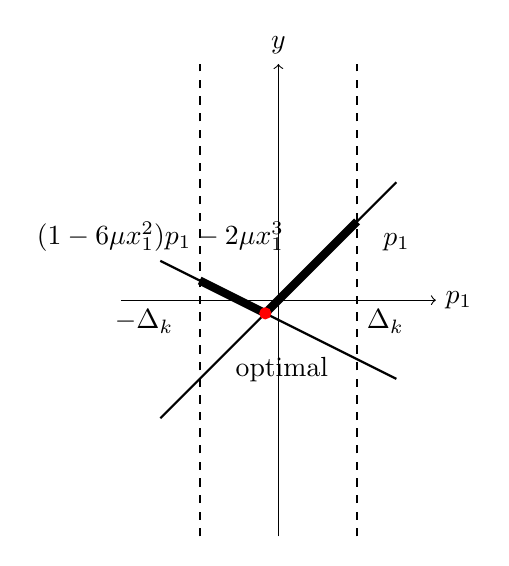
\begin{tikzpicture}
% Axes
    \draw[->] (-2,0) -- (2,0) node[right] {$p_1$}; % x-axis
    \draw[->] (0,-3) -- (0,3) node[above] {$y$}; % y-axis

    % Adjustable x1 value
    \def\xone{0.5} % Set x1 value (you can adjust this)

    % Vertical line for x = x1
    \draw[thick, dashed] (1,-3) -- (1,3); % x1 vertical line
    \node[below right] at (1,0) {$\Delta_k$};

    % Vertical line for x = x1
    \draw[thick, dashed] (-1,-3) -- (-1,3); % x1 vertical line
    \node[below right] at (-2.2,0) {$-\Delta_k$};

    % Line 1
    \draw[thick, domain=-1.5:1.5, samples=100] 
        plot (\x, {(1 - 6*(\xone)^2)*\x - 2*(\xone)^3}); % 
    \draw[line width=3pt, domain=-1:-\xone/3, samples=100] 
        plot (\x, {(1 - 6*(\xone)^2)*\x - 2*(\xone)^3});
    \node[above] at (-1.5,0.5) {$(1 - 6\mu x_1^2)p_1 - 2\mu x_1^3$};

    % Line 2
    \draw[thick, domain=-1.5:1.5, samples=100] 
        plot (\x, \x); 
    \draw[line width=3pt, domain=-\xone/3:1, samples=100] 
        plot (\x, \x);
    \node[above] at (1.5,0.5) {$p_1$};

     % Red point at (1, 1)
    \filldraw[red] (-\xone/3,-\xone/3) circle (2pt); % Draws a red filled circle at (1, 1)

    % Label for the red point
    \node[above right] at (-\xone/3-0.5,-\xone/3-1) {optimal };

    \end{tikzpicture}
%%%  \end{adjustbox}       %
\end{subfigure}%
   \hspace{0.02\textwidth}
  \begin{subfigure}[b]{0.30\textwidth}
  \centering
  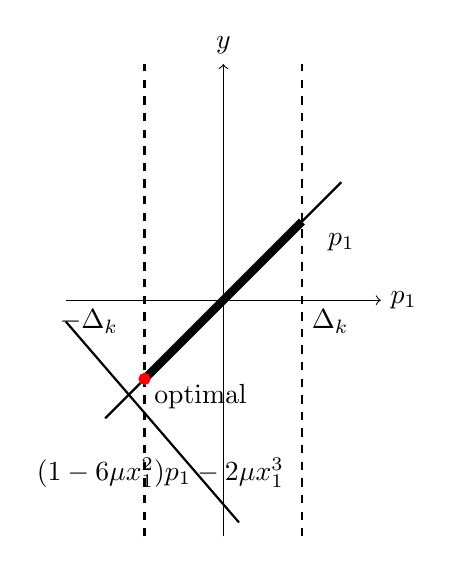
\begin{tikzpicture}
% Axes
    \draw[->] (-2,0) -- (2,0) node[right] {$p_1$}; % x-axis
    \draw[->] (0,-3) -- (0,3) node[above] {$y$}; % y-axis

    % Adjustable x1 value
    \def\xone{0.6} % Set x1 value (you can adjust this)

    % Vertical line for x = x1
    \draw[thick, dashed] (1,-3) -- (1,3); % x1 vertical line
    \node[below right] at (1,0) {$\Delta_k$};

    % Vertical line for x = x1
    \draw[thick, dashed] (-1,-3) -- (-1,3); % x1 vertical line
    \node[below right] at (-2.2,0) {$-\Delta_k$};

    % Line 1
    \draw[thick, domain=-2:0.2, samples=100] 
        plot (\x, {(1 - 6*(\xone)^2)*\x - 12*(\xone)^3}); % 
    \node[above] at (-0.8,-2.5) {$(1 - 6\mu x_1^2)p_1 - 2\mu x_1^3$};

    % Line 2
    \draw[thick, domain=-1.5:1.5, samples=100] 
        plot (\x, \x); 
    \draw[line width=3pt, domain=-1:1, samples=100] 
        plot (\x, \x);
    \node[above] at (1.5,0.5) {$p_1$};

     % Red point at (1, 1)
    \filldraw[red] (-1,-1) circle (2pt); % Draws a red filled circle at (1, 1)

    % Label for the red point
    \node[above right] at (-1,-1.5) {optimal };

    \end{tikzpicture}
%%%  \end{adjustbox}       %
\end{subfigure}%
\hspace{-0.01\textwidth}
\begin{subfigure}[b]{0.30\textwidth}
\centering
  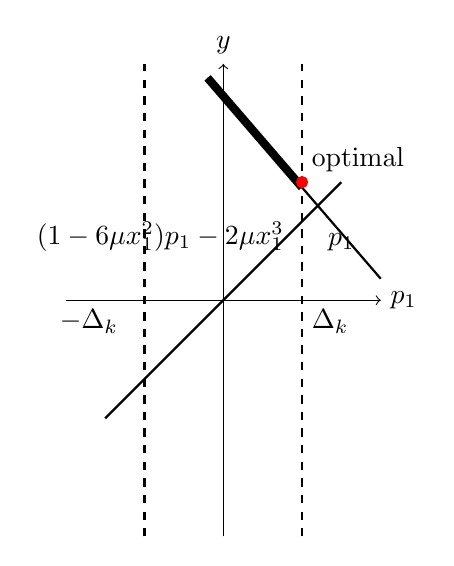
\begin{tikzpicture}
% Axes
    \draw[->] (-2,0) -- (2,0) node[right] {$p_1$}; % x-axis
    \draw[->] (0,-3) -- (0,3) node[above] {$y$}; % y-axis

    % Adjustable x1 value
    \def\xone{-0.6} % Set x1 value (you can adjust this)

    % Vertical line for x = x1
    \draw[thick, dashed] (1,-3) -- (1,3); % x1 vertical line
    \node[below right] at (1,0) {$\Delta_k$};

    % Vertical line for x = x1
    \draw[thick, dashed] (-1,-3) -- (-1,3); % x1 vertical line
    \node[below right] at (-2.2,0) {$-\Delta_k$};

    % Line 1
    \draw[thick, domain=-0.2:2, samples=100] 
        plot (\x, {(1 - 6*(\xone)^2)*\x - 12*(\xone)^3}); % 
      \draw[line width=3pt, domain=-0.2:1, samples=100] 
        plot (\x, {(1 - 6*(\xone)^2)*\x - 12*(\xone)^3});  
    \node[above] at (-0.8,0.5) {$(1 - 6\mu x_1^2)p_1 - 2\mu x_1^3$};

    % Line 2
    \draw[thick, domain=-1.5:1.5, samples=100] 
        plot (\x, \x); 

    \node[above] at (1.5,0.5) {$p_1$};

     % Red point at (1, 1)
    \filldraw[red] (1,1.5) circle (2pt); % Draws a red filled circle at (1, 1)

    % Label for the red point
    \node[above right] at (1,1.5) {optimal };

    \end{tikzpicture}
%%%  \end{adjustbox}       %
\end{subfigure}%
\caption{Visualization of cases where $1-6\mu x_1^2 \leq 0$. The graph illustrates three distinct scenarios, each corresponding to different values of $x_1$, showcasing the various intersections of the two linear functions. The bold segments represent the composite \textit{max} function, while the \textit{min} points are denoted by red dots. The intersection is $\hat{p}_1 = -x_1/3$.}
\label{fig:case-visualization01}
\end{figure}

\begin{figure}[H]
  \centering
  \begin{subfigure}[b]{0.30\textwidth}
  \centering
%%%    \begin{adjustbox}{width=\linewidth} % rescale box
    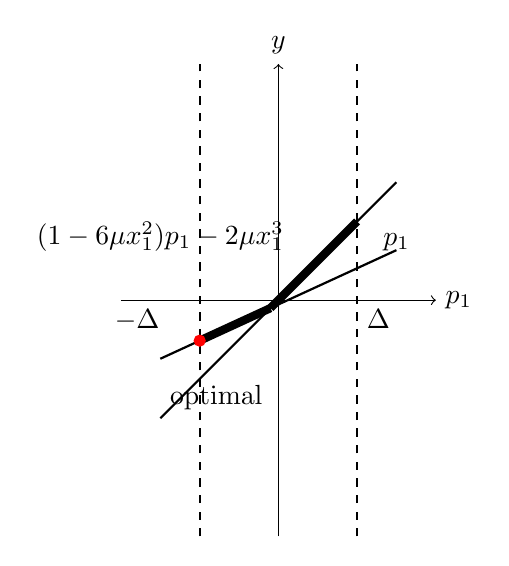
\begin{tikzpicture}
% Axes
    \draw[->] (-2,0) -- (2,0) node[right] {$p_1$}; % x-axis
    \draw[->] (0,-3) -- (0,3) node[above] {$y$}; % y-axis

    % Adjustable x1 value
    \def\xone{0.3} % Set x1 value (you can adjust this)

    % Vertical line for x = x1
    \draw[thick, dashed] (1,-3) -- (1,3); % x1 vertical line
    \node[below right] at (1,0) {$\Delta$};

    % Vertical line for x = x1
    \draw[thick, dashed] (-1,-3) -- (-1,3); % x1 vertical line
    \node[below right] at (-2.2,0) {$-\Delta$};

    % Line 1
    \draw[thick, domain=-1.5:1.5, samples=100] 
        plot (\x, {(1 - 6*(\xone)^2)*\x - 2*(\xone)^3}); % 
    \draw[line width=3pt, domain=-1:-\xone/3, samples=100] 
        plot (\x, {(1 - 6*(\xone)^2)*\x - 2*(\xone)^3});
    \node[above] at (-1.5,0.5) {$(1 - 6\mu x_1^2)p_1 - 2\mu x_1^3$};

    % Line 2
    \draw[thick, domain=-1.5:1.5, samples=100] 
        plot (\x, \x); 
    \draw[line width=3pt, domain=-\xone/3:1, samples=100] 
        plot (\x, \x);
    \node[above] at (1.5,0.5) {$p_1$};

     % Red point at (1, 1)
    \filldraw[red] (-1,-1 + 6*\xone^2 - 2*\xone^3) circle (2pt); % Draws a red filled circle at (1, 1)

    % Label for the red point
    \node[above right] at (-1.5,-1 + 6*\xone^2 - 2*\xone^3-1) {optimal };

    \end{tikzpicture}
%%%  \end{adjustbox}       %
\end{subfigure}%
   \hspace{0.02\textwidth}
  \begin{subfigure}[b]{0.30\textwidth}
  \centering
  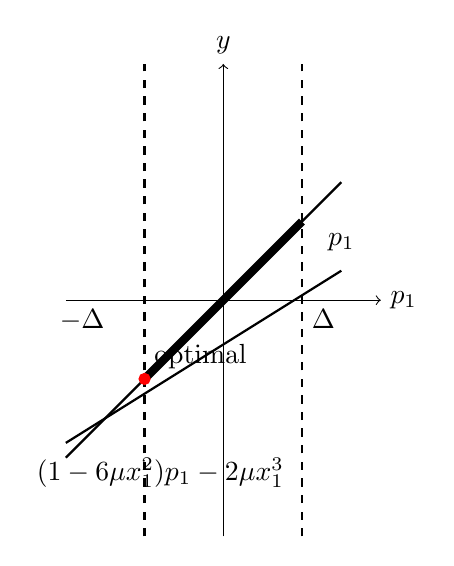
\begin{tikzpicture}
% Axes
    \draw[->] (-2,0) -- (2,0) node[right] {$p_1$}; % x-axis
    \draw[->] (0,-3) -- (0,3) node[above] {$y$}; % y-axis

    % Adjustable x1 value
    \def\xone{0.25} % Set x1 value (you can adjust this)

    % Vertical line for x = x1
    \draw[thick, dashed] (1,-3) -- (1,3); % x1 vertical line
    \node[below right] at (1,0) {$\Delta$};

    % Vertical line for x = x1
    \draw[thick, dashed] (-1,-3) -- (-1,3); % x1 vertical line
    \node[below right] at (-2.2,0) {$-\Delta$};

    % Line 1
    \draw[thick, domain=-2:1.5, samples=100] 
        plot (\x, {(1 - 6*(\xone)^2)*\x - 36*(\xone)^3}); % 
    \node[above] at (-0.8,-2.5) {$(1 - 6\mu x_1^2)p_1 - 2\mu x_1^3$};

    % Line 2
    \draw[thick, domain=-2:1.5, samples=100] 
        plot (\x, \x); 
    \draw[line width=3pt, domain=-1:1, samples=100] 
        plot (\x, \x);
    \node[above] at (1.5,0.5) {$p_1$};

     % Red point at (1, 1)
    \filldraw[red] (-1,-1) circle (2pt); % Draws a red filled circle at (1, 1)

    % Label for the red point
    \node[above right] at (-1,-1) {optimal };

    \end{tikzpicture}
%%%  \end{adjustbox}       %
\end{subfigure}%
\hspace{-0.01\textwidth}
\begin{subfigure}[b]{0.30\textwidth}
\centering
  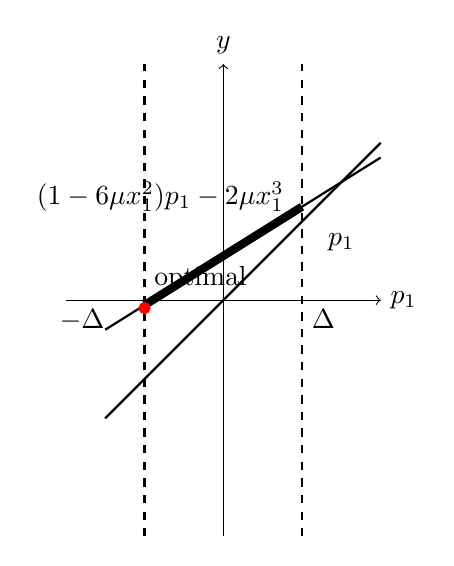
\begin{tikzpicture}
% Axes
    \draw[->] (-2,0) -- (2,0) node[right] {$p_1$}; % x-axis
    \draw[->] (0,-3) -- (0,3) node[above] {$y$}; % y-axis

    % Adjustable x1 value
    \def\xone{-0.25} % Set x1 value (you can adjust this)

    % Vertical line for x = x1
    \draw[thick, dashed] (1,-3) -- (1,3); % x1 vertical line
    \node[below right] at (1,0) {$\Delta$};

    % Vertical line for x = x1
    \draw[thick, dashed] (-1,-3) -- (-1,3); % x1 vertical line
    \node[below right] at (-2.2,0) {$-\Delta$};

    % Line 1
    \draw[thick, domain=-1.5:2, samples=100] 
        plot (\x, {(1 - 6*(\xone)^2)*\x - 36*(\xone)^3}); % 
      \draw[line width=3pt, domain=-1:1, samples=100] 
        plot (\x, {(1 - 6*(\xone)^2)*\x - 36*(\xone)^3});  
    \node[above] at (-0.8,1) {$(1 - 6\mu x_1^2)p_1 - 2\mu x_1^3$};

    % Line 2
    \draw[thick, domain=-1.5:2, samples=100] 
        plot (\x, \x); 

    \node[above] at (1.5,0.5) {$p_1$};

     % Red point at (1, 1)
    \filldraw[red] (-1,-0.1) circle (2pt); % Draws a red filled circle at (1, 1)

    % Label for the red point
    \node[above right] at (-1,0) {optimal };

    \end{tikzpicture}
%%%  \end{adjustbox}       %
\end{subfigure}%
\caption{Visualization of cases where $1-6\mu x_1^2 > 0$. In all three scenarios depicted, the optimal solution converges to the same \textit{min-max} point at $\hat{p}_1=-\Delta$, regardless of the specific intersection patterns of the linear functions.}
\label{fig:case-visualization02}
\end{figure}
We then analyze different cases distinguished by the sign of $1-6\mu x_1^2$. For clarity, these scenarios are illustrated in~\prettyref{fig:case-visualization01}, which provides an intuitive understanding of the process. The figure demonstrates how we first identify the \textit{max} segment of these two lines and then extract the \textit{min} point of the resulting composite line, thereby solving the constrained \textit{min-max} problem. Thus, we conclude that:
\begin{align}
|x_1| > 1/\sqrt{6\mu} &\Rightarrow \hat{p}_1  = \mathrm{clip}(\frac{-x_1}{3},\Delta_k) \\
-1/\sqrt{6\mu}\leq x_1 \leq 1/\sqrt{6\mu} &\Rightarrow \hat{p}_1  = -\Delta_k,
\end{align}
which indicates that $\hat{p}_1$ will always take a step towards $x_1=-1/\sqrt{6\mu}$, either with length $|x_1/3|$ or the trust region radius $|\Delta_k|$. The \textbf{clip} function is defined by $\mathrm{clip}(a,b) = \max\{\min\{a,b\},-b\}$. Consequently, $x_2$ would converge to zero by taking the value consistent in Equation~\eqref{eq:case:mu_1} and~\eqref{eq:case:mu_2}. We thus conclude that the proposed algorithm exhibits dynamic convergence towards a final stable point, $(-1/\sqrt{6\mu},0)$.

The radius of the trust region is dynamically adjusted based on the magnitude of decrease in the merit function induced by the trial step. Through a similar deduction on the merit function, with an appropriately chosen $x_2$, we obtain:
\begin{equation}
    \phi_1 = x_1 + \mu[x_1^3-x_2]^-+\mu[x_1^3+x_2]^- = 
    \begin{cases}
        x_1 - 2\mu x_1^3,  & \text{for } x_1 < 0 \\
        x_1, & \text{for } x_1 \geq 0
    \end{cases}
\end{equation}
The stationary point of $\phi_1$ is obtained at $x_1 = -1/\sqrt{6\mu}$ and $|x_2|\leq|x_1^3|$. In practice, we employ a large value for $\mu$, resulting in $x_2$ being a negligibly small quantity, approaching zero due to the cubic relationship. This stationary point aligns with the stable point of our algorithm.

\end{document}


